\documentclass[11pt]{book}
\oddsidemargin 0in
\evensidemargin 0in
\marginparwidth 0in
\textheight 8in
\textwidth 6.5in
\topmargin 0in
\usepackage{amssymb,amsmath,amsthm,fancyhdr,supertabular,longtable,hhline}
\usepackage{colortbl}
\usepackage{import, multicol,boxedminipage}
\usepackage{chapterfolder}
\usepackage[metapost,truebbox]{mfpic}
\usepackage[pdflatex]{graphicx}
\usepackage{makeidx}
\usepackage[colorlinks, hyperindex, plainpages=false, linkcolor=blue, urlcolor=blue, pdfpagelabels]{hyperref}
\usepackage[all]{hypcap}
\usepackage{cancel}
\usepackage{sectsty}
\usepackage{textcomp}
\allsectionsfont{\mdseries \scshape}
\definecolor{ResultColor}{gray}{0.9}
\theoremstyle{definition}  % this prevents the text in definitions, theorems, and corollaries from being italicized
\newtheorem{defn}{Definition}[chapter]
\newtheorem{thm}{Theorem}[chapter]
\newtheorem{cor}[thm]{Corollary}
\newtheorem{eqn}{Equation}[chapter]
\newtheorem{ex}{Example}[section]
\setlength{\parindent}{0in}
\newcommand{\bbm}{\begin{boxedminipage}{6.41in}}
\newcommand{\ebm}{\end{boxedminipage}}
\newcounter{HW}
\newcounter{HWindent}

\begin{document}
\chapter{\sc Exponential and Logarithmic Functions}

\section{Introduction to Exponential and Logarithmic Functions}

\mfpicnumber{1}

\opengraphsfile{IntroExpLogs}

\setcounter{footnote}{0}

\label{IntroExpLogs}

Of all of the  functions we study in this text, exponential and logarithmic functions are possibly the ones which impact everyday life the most.\footnote{Take a class in Differential Equations and you'll see why.} This section will introduce us to these functions while the rest of the chapter will more thoroughly explore their properties.  Up to this point, we have dealt with functions which involve terms like $x^2$ or $x^{2/3}$, in other words, terms of the form  $x^{p}$ where the base of the term, $x$, varies but the exponent of each term, $p$, remains constant.  In this chapter, we study functions of the form $f(x) = b^{x}$ where the base $b$ is a constant and the exponent $x$ is the variable.  We start our exploration of these functions with $f(x) = 2^{x}$. (Apparently this is a tradition.  Every College Algebra book we have ever read starts with $f(x) = 2^{x}$.) We make a table of values, plot the points and connect them in a pleasing fashion.

\hspace{1in} \begin{tabular}{m{2.7in}m{3in}}

\setlength{\extrarowheight}{4pt}
\[ \begin{array}{|r||r|r|}  

\hline

 x & f(x) & (x,f(x)) \\ \hline
-3  & 2^{-3} = \frac{1}{8} & \left(-3, \frac{1}{8} \right) \\ [2pt] \hline
-2  & 2^{-2} = \frac{1}{4} &  \left(-2, \frac{1}{4} \right) \\ [2pt] \hline
-1 & 2^{-1} &  \left(-1, \frac{1}{2} \right) \\ [2pt]  \hline
0  & 2^{0} = 1 & ( 0 ,1) \\  \hline
1 & 2^{1} = 2 & ( 1, 2) \\  \hline
2  & 2^{2} = 4 & (2,4) \\  \hline
3  & 2^{3}=8 & (3, 8) \\  \hline
\end{array} \] 
\setlength{\extrarowheight}{2pt}

&

\begin{mfpic}[13]{-4}{4}{-1}{9}
\point[2pt]{(-3,0.125), (-2,0.25), (-1,0.5), (0,1), (1,2), (2,4), (3,8)}
\axes
\tlabel[cc](4,-0.5){\scriptsize $x$}
\tlabel[cc](0.5,9){\scriptsize $y$}
\tcaption{\scriptsize $y = f(x) = 2^{x}$}
\xmarks{-3,-2,-1,1,2,3}
\ymarks{1,2,3,4,5,6,7,8}
\tlpointsep{4pt}
\axislabels {x}{{\tiny $-3 \hspace{7pt}$} -3, {\tiny $-2 \hspace{7pt}$} -2, {\tiny $-1 \hspace{7pt}$} -1, {\tiny $1$} 1, {\tiny $2$} 2, {\tiny $3$} 3}
\axislabels {y}{{\tiny $1$} 1, {\tiny $2$} 2, {\tiny $3$} 3, {\tiny $4$} 4, {\tiny $5$} 5, {\tiny $6$} 6, {\tiny $7$} 7, {\tiny $8$} 8}
\arrow \reverse \arrow \function{-3.5, 3.1, 0.1}{2**x}
\end{mfpic} \\

\end{tabular}

A few remarks about the graph of $f(x) = 2^{x}$ which we have constructed are in order.  As $x \rightarrow -\infty$ and attains values like $x = -100$ or $x=-1000$, the function $f(x) = 2^{x}$ takes on values like $f(-100) = 2^{-100} = \frac{1}{2^{100}}$ or $f(-1000) = 2^{-1000} = \frac{1}{2^{1000}}$.  In other words, as $x \rightarrow -\infty$, \[2^{x} \approx \frac{1}{\mbox{very big $(+)$}}  \approx \mbox{very small $(+)$}\]  So as $x \rightarrow -\infty$, $2^{x} \rightarrow 0^{+}$.  This is represented graphically using the $x$-axis (the line $y = 0$) as a horizontal asymptote.  On the flip side, as $x \rightarrow \infty$, we find $f(100) = 2^{100}$, $f(1000) = 2^{1000}$, and so on, thus $2^{x} \rightarrow \infty$. As a result, our graph suggests the range of $f$ is $(0,\infty)$.  The graph of $f$ passes the Horizontal Line Test which means $f$ is one-to-one and hence invertible.  We also note that when we `connected the dots in a pleasing fashion', we have made the implicit assumption that $f(x) = 2^{x}$ is continuous\footnote{Recall that this means there are no holes or other kinds of breaks in the graph.} and has a domain of all real numbers.  In particular, we have suggested that things like $2^{\sqrt{3}}$ exist as real numbers.  We should take a moment to discuss what something like $2^{\sqrt{3}}$ might mean, and refer the interested reader to a solid course in Calculus for a more rigorous explanation.  The number $\sqrt{3} = 1.73205 \ldots$ is an irrational number\footnote{You can actually prove this by considering the polynomial $p(x) = x^2-3$ and showing it has no rational zeros by applying Theorem \ref{RZT}.} and as such, its decimal representation neither repeats nor terminates.  We can, however, approximate $\sqrt{3}$ by terminating decimals, and it stands to reason\footnote{This is where Calculus and continuity come into play.} we can use these to approximate $2^{\sqrt{3}}$.  For example, if we approximate $\sqrt{3}$ by $1.73$, we can approximate $2^{\sqrt{3}} \approx 2^{1.73} = 2^{\frac{173}{100}} = \sqrt[100]{2^{173}}$. It is not, by any means, a pleasant number, but it is at least a number that we understand in terms of powers and roots.  It also stands to reason that better and better approximations of $\sqrt{3}$ yield better and better approximations of $2^{\sqrt{3}}$, so the value of $2^{\sqrt{3}}$ should be the result of this sequence of approximations.\footnote{Want more information?  Look up ``convergent sequences'' on the Internet.}
  
\smallskip

Suppose we wish to study the family of functions $f(x) = b^{x}$.  Which bases $b$ make sense to study?  We find that we run into difficulty if $b < 0$.  For example, if $b = -2$, then the function $f(x) = (-2)^{x}$ has trouble, for instance, at $x = \frac{1}{2}$ since $(-2)^{1/2} = \sqrt{-2}$ is not a real number. In general, if $x$ is any rational number with an even denominator, then $(-2)^{x}$ is not defined, so we must restrict our attention to bases $b \geq 0$.  What about $b = 0$?  The function $f(x) = 0^{x}$ is undefined for $x \leq 0$ because we cannot divide by $0$ and $0^{0}$ is an indeterminant form.  For $x > 0$, $0^{x} = 0$ so the function  $f(x) = 0^{x}$ is the same as the function $f(x) = 0$, $x > 0$. \phantomsection \label{indeterminantformtwo} We know everything we can possibly know about this function, so we exclude it from our investigations.  The only other base we exclude is $b=1$, since the function $f(x) = 1^{x} = 1$ is, once again, a function we have already studied.  We are now ready for our definition of exponential functions.

\smallskip


\colorbox{ResultColor}{\bbm

\begin{defn} \label{expfcndefn}  A function of the form $f(x) = b^{x}$ where $b$ is a fixed real number, $b > 0$, $b \neq 1$ is called a \index{function ! exponential} \index{exponential function ! definition of} \textbf{base \emph{b} exponential function}.

\end{defn}


\ebm}
\smallskip

We leave it to the reader to verify\footnote{Meaning, graph some more examples on your own.} that if $b > 1$, then the exponential function $f(x) = b^{x}$ will share the same basic shape and characteristics as $f(x) = 2^{x}$.  What if $0 < b < 1$?  Consider $g(x) = \left(\frac{1}{2}\right)^{x}$.  We could certainly build a table of values and connect the points, or we could take a step back and note that $g(x) = \left(\frac{1}{2}\right)^{x} = \left(2^{-1}\right)^{x} = 2^{-x} = f(-x)$, where $f(x) = 2^{x}$.  Thinking back to Section \ref{Transformations}, the graph of $f(-x)$ is obtained from the graph of $f(x)$ by reflecting it across the $y$-axis. We get

\[\begin{array}{ccc}

\begin{mfpic}[10]{-4}{4}{-1}{9}
\point[2pt]{(-3,0.125), (-2,0.25), (-1,0.5), (0,1), (1,2), (2,4), (3,8)}
\axes
\tlabel[cc](4,-0.5){\scriptsize $x$}
\tlabel[cc](0.5,9){\scriptsize $y$}
\tcaption{\scriptsize $y = f(x) = 2^{x}$}
\xmarks{-3,-2,-1,1,2,3}
\ymarks{1,2,3,4,5,6,7,8}
\tlpointsep{4pt}
\axislabels {x}{{\tiny $-3 \hspace{7pt}$} -3, {\tiny $-2 \hspace{7pt}$} -2, {\tiny $-1 \hspace{7pt}$} -1, {\tiny $1$} 1, {\tiny $2$} 2, {\tiny $3$} 3}
\axislabels {y}{{\tiny $1$} 1, {\tiny $2$} 2, {\tiny $3$} 3, {\tiny $4$} 4, {\tiny $5$} 5, {\tiny $6$} 6, {\tiny $7$} 7, {\tiny $8$} 8}
\arrow \reverse \arrow \function{-3.5, 3.1, 0.1}{2**x}
\end{mfpic}

&

\stackrel{\stackrel{\mbox{\scriptsize reflect across $y$-axis}}{\xrightarrow{\hspace{1in}}}}{\mbox{ \scriptsize multiply each $x$-coordinate by $-1$}} 

&

\begin{mfpic}[10]{-4}{4}{-1}{9}
\point[2pt]{(3,0.125), (2,0.25), (1,0.5), (0,1), (-1,2), (-2,4), (-3,8)}
\axes
\tlabel[cc](4,-0.5){\scriptsize $x$}
\tlabel[cc](0.5,9){\scriptsize $y$}
\tcaption{\scriptsize $y = g(x) = 2^{-x} = \left(\frac{1}{2}\right)^{x}$}
\xmarks{-3,-2,-1,1,2,3}
\ymarks{1,2,3,4,5,6,7,8}
\tlpointsep{4pt}
\axislabels {x}{{\tiny $-3 \hspace{7pt}$} -3, {\tiny $-2 \hspace{7pt}$} -2, {\tiny $-1 \hspace{7pt}$} -1, {\tiny $1$} 1, {\tiny $2$} 2, {\tiny $3$} 3}
\axislabels {y}{{\tiny $1$} 1, {\tiny $2$} 2, {\tiny $3$} 3, {\tiny $4$} 4, {\tiny $5$} 5, {\tiny $6$} 6, {\tiny $7$} 7, {\tiny $8$} 8}
\arrow \reverse \arrow \function{-3.1, 3.5, 0.1}{(0.5)**x}
\end{mfpic} \\

\end{array}\]

We see that the domain and range of $g$ match that of $f$, namely $(-\infty, \infty)$ and $(0,\infty)$, respectively. Like $f$, $g$ is also one-to-one.  Whereas $f$ is always increasing, $g$ is always decreasing.  As a result, as $x \rightarrow -\infty$, $g(x) \rightarrow \infty$, and on the flip side, as $x \rightarrow \infty$, $g(x) \rightarrow 0^{+}$.  It shouldn't be too surprising that for all choices of the base $0 < b < 1$, the graph of $y=b^{x}$ behaves similarly to the graph of $g$.  We summarize the basic properties of exponential functions in the following theorem.\footnote{The proof of which, like many things discussed in the text, requires Calculus.}

\smallskip

\colorbox{ResultColor}{\bbm

\begin{thm} \label{expfcnprops} \textbf{Properties of Exponential Functions:} Suppose $f(x) = b^{x}$. \index{exponential function ! graphical properties of}

\begin{itemize}

\item  The domain of $f$ is $(-\infty, \infty)$ and the range of $f$ is $(0, \infty)$.

\item  $(0,1)$ is on the graph of $f$ and $y=0$ is a horizontal asymptote to the graph of $f$.

\item  $f$ is one-to-one, continuous and smooth\footnote{Recall that this means the graph of $f$ has no sharp turns or corners.}

\end{itemize}

\begin{tabular}{m{2.5in}m{2.5in}}

\begin{itemize}

\item  If $b > 1$:

\begin{itemize}

\item  $f$ is always increasing

\item  As $x \rightarrow -\infty$, $f(x) \rightarrow 0^{+}$

\item  As $x \rightarrow \infty$, $f(x) \rightarrow \infty$

\item  The graph of $f$ resembles:

\begin{center}

\begin{mfpic}[10]{-3}{3}{-1}{5}

\axes

\ymarks{1}

\arrow \reverse \arrow \function{-2.3,2.3,0.1}{2**x}

\tcaption{\scriptsize $y = b^{x}$, $b > 1$}

\end{mfpic}

\end{center}

\end{itemize}

\end{itemize}

&
\begin{itemize}

\item  If $0<b<1$:

\begin{itemize}

\item  $f$ is always decreasing

\item  As $x \rightarrow -\infty$, $f(x) \rightarrow \infty$

\item  As $x \rightarrow \infty$, $f(x) \rightarrow 0^{+}$

\item  The graph of $f$ resembles:

\begin{center}

\begin{mfpic}[10]{-3}{3}{-1}{5}

\axes

\ymarks{1}

\arrow \reverse \arrow \function{-2.3,2.3,0.1}{(0.5)**x}

\tcaption{\scriptsize $y = b^{x}$, $0 < b < 1$}

\end{mfpic}


\end{center}

\end{itemize}

\end{itemize} \\

\end{tabular}

\end{thm}

\ebm}

\smallskip

Of all of the bases for exponential functions, two occur the most often in scientific circles.  The first, base $10$, is often called the \index{exponential function ! common base} \index{common base} \textbf{common base}.  The second base is an irrational number, $e \approx 2.718$, called the \index{natural base} \index{exponential function ! natural base} \textbf{natural base}.  We will more formally discuss the origins of this number in Section \ref{ExpLogApplications}.  For now, it is enough to know that since $e > 1$, $f(x) = e^{x}$ is an increasing exponential function.  The following examples give us an idea how these functions are used in the wild.

\begin{ex}  \label{cardepreciationex} The value of a car can be modeled by $V(x) = 25\left(\frac{4}{5}\right)^{x}$, where $x \geq 0$ is age of the car in years and $V(x)$ is the value in thousands of dollars. \index{depreciation}

\begin{enumerate}

\item  Find and interpret $V(0)$.

\item  Sketch the graph of $y=V(x)$ using transformations.

\item  Find and interpret the horizontal asymptote of the graph you found in 2.

\end{enumerate}

{\bf Solution.}

\begin{enumerate}

\item  To find $V(0)$, we replace $x$ with $0$ to obtain $V(0) = 25\left(\frac{4}{5}\right)^{0} = 25$.  Since $x$ represents the age of the car in years, $x=0$ corresponds to the car being brand new.  Since $V(x)$ is measured in thousands of dollars, $V(0)=25$ corresponds to a value of $\$ 25,\!000$.  Putting it all together, we interpret $V(0)=25$ to mean the purchase price of the car was $\$25,\!000$.

\item  To graph $y=25\left(\frac{4}{5}\right)^{x}$,  we start with the basic exponential function $f(x)=\left(\frac{4}{5}\right)^{x}$.  Since the base $b = \frac{4}{5}$ is between $0$ and $1$, the graph of $y=f(x)$ is decreasing.  We plot the $y$-intercept $(0,1)$ and two other points, $\left(-1, \frac{5}{4}\right)$ and $\left(1, \frac{4}{5}\right)$, and label the horizontal asymptote $y=0$.  To obtain $V(x) = 25\left(\frac{4}{5}\right)^{x}$, $x \geq 0$, we multiply the output from $f$ by $25$, in other words, $V(x) = 25 f(x)$. In accordance with Theorem \ref{vscalings}, this results in a vertical stretch by a factor of $25$.  We multiply all of the $y$ values in the graph by $25$ (including the $y$ value of the horizontal asymptote) and obtain the points $\left(-1,\frac{125}{4}\right)$, $(0,25)$ and $(1,20)$. The horizontal asymptote remains $y=0$. Finally, we restrict the domain to $[0,\infty)$ to fit with the applied domain given to us.  We have the result below.

\[\begin{array}{ccc}

\begin{mfpic}[10][20]{-4}{4}{-1}{3}
\point[2pt]{(0,1),(1,0.8), (-1,1.25)}
\axes
\tlabel[cc](1,1.25){\tiny $(0,1)$}
\tlabel[cc](0,-1.5){\tiny H.A. $y=0$}
\tlabel[cc](4,-0.5){\tiny $x$}
\tlabel[cc](0.5,3){\tiny $y$}
\tcaption{\scriptsize $y = f(x)=\left(\frac{4}{5}\right)^{x}$}
\ymarks{1,2}
\xmarks{-3,-2,-1,1,2,3}
\tlpointsep{4pt}
\axislabels {x}{{\tiny $-3 \hspace{7pt}$} -3, {\tiny $-2 \hspace{7pt}$} -2, {\tiny $-1 \hspace{7pt}$} -1, {\tiny $1$} 1, {\tiny $2$} 2, {\tiny $3$} 3}
\axislabels {y}{{\tiny $2$} 2}
\arrow \reverse \arrow \function{-4, 4, 0.1}{(0.8)**x}
\end{mfpic}

&

\stackrel{\stackrel{\mbox{\scriptsize vertical scale by a factor of $25$ }}{\xrightarrow{\hspace{1.75in}}}}{\mbox{ \scriptsize multiply each $y$-coordinate by $25$}} 

&

\begin{mfpic}[10]{-1}{7}{-1}{7}
\point[2pt]{(0,5),(1,4)}
\axes
\tlabel[cc](-1.5,5){\tiny $(0,25)$}
\tlabel[cc](4,-1.5){\tiny H.A. $y=0$}
\tlabel[cc](7,-0.5){\tiny $x$}
\tlabel[cc](0.5,7){\tiny $y$}
\tcaption{\scriptsize $y = V(x)=25 f(x)$, $x \geq 0$}
\ymarks{1,2,3,4,5,6}
\xmarks{1,2,3,4,5,6}
\tlpointsep{4pt}
\axislabels {x}{{\tiny $1$} 1, {\tiny $2$} 2, {\tiny $3$} 3, {\tiny $4$} 4, {\tiny $5$} 5, {\tiny $6$} 6}
\axislabels {y}{{\tiny $5$} 1, {\tiny $10$} 2, {\tiny $15$} 3, {\tiny $20$} 4, {\tiny $30$} 6}
\arrow \function{0, 7, 0.1}{5*((0.8)**x)}
\end{mfpic} \\

\end{array}\]

\item  We see from the graph of $V$ that its horizontal asymptote is $y=0$.  (We leave it to reader to verify this analytically by thinking about what happens as we take larger and larger powers of $\frac{4}{5}$.)  This means as the car gets older, its value diminishes to $0$.  \qed
 
\end{enumerate}

\end{ex}

The function in the previous example is often called a `decay curve'.  Increasing exponential functions are used to model `growth curves' and we shall see several different examples of those in Section \ref{ExpLogApplications}.  For now, we present another common decay curve which will serve as the basis for further study of exponential functions.  Although it may look more complicated than the previous example, it is actually just a basic exponential function which has been modified by a few transformations from Section \ref{Transformations}.

\begin{ex}  \label{exptempex} According to \href{http://en.wikipedia.org/wiki/Heat_transfer#Newton.27s_law_of_cooling}{\underline{Newton's Law of Cooling}}\footnote{We will discuss this in greater detail in Section \ref{ExpLogApplications}.} the temperature of coffee $T$ (in degrees Fahrenheit) $t$ minutes after it is served can be modeled by $T(t) = 70 + 90 e^{-0.1 t}$. \index{Newton's Law of Cooling}

\begin{enumerate}

\item  Find and interpret $T(0)$.

\item  Sketch the graph of $y = T(t)$ using transformations.

\item  Find and interpret the horizontal asymptote of the graph.

\end{enumerate}

{\bf Solution.}

\begin{enumerate}

\item  To find $T(0)$, we replace every occurrence of the independent variable $t$ with $0$ to obtain  $T(0) =70 + 90 e^{-0.1 (0)} = 160$.  This means that the coffee was served at $160^{\circ}\mbox{F}$.

\item  To graph $y = T(t)$ using transformations, we start with the basic function, $f(t)=e^{t}$.  As we have already remarked, $e \approx 2.718 > 1$ so the graph of $f$ is an increasing exponential with $y$-intercept $(0,1)$ and horizontal asymptote $y = 0$.  The points $\left(-1, e^{-1}\right) \approx (-1,0.37)$ and $(1,e) \approx (1,2.72)$ are also on the graph.  Since the formula $T(t)$ looks rather complicated, we rewrite $T(t)$ in the form presented in Theorem  \ref{transformationsthm} and use that result to track the changes to our three points and the horizontal asymptote.  We have \[T(t) = 70 + 90e^{-0.1t} = 90e^{-0.1t}+70 = 90 f(-0.1t)+70\]  Multiplication of the input to $f$, $t$, by $-0.1$ results in a horizontal expansion by a factor of $10$ as well as a reflection about the $y$-axis.  We divide each of the $x$ values of our points by $-0.1$ (which amounts to multiplying them by $-10$) to obtain $\left(10,e^{-1}\right)$, $(0,1)$, and $\left(-10, e\right)$.  Since none of these changes affected the $y$ values, the horizontal asymptote remains $y = 0$.  Next, we see that the output from $f$ is being multiplied by $90$.  This results in a vertical stretch by a factor of $90$.  We multiply the $y$-coordinates by $90$ to obtain $\left(10,90e^{-1}\right)$, $(0,90)$, and $\left(-10, 90e\right)$. We also multiply the $y$ value of the horizontal asymptote $y=0$ by $90$, and it remains $y=0$.  Finally, we add $70$ to all of the $y$-coordinates, which shifts the graph upwards to obtain $\left(10,90e^{-1} + 70\right) \approx (10, 103.11)$, $(0,160)$, and $\left(-10, 90e+ 70\right) \approx (-10,314.64)$.  Adding $70$ to the horizontal asymptote shifts it upwards as well to $y=70$.  We connect these three points using the same shape in the same direction as in the graph of $f$ and, last but not least, we restrict the domain to match the applied domain $[0, \infty)$.  The result is below.  


\[\begin{array}{ccc}

\begin{mfpic}[10]{-4}{4}{-1}{8}
\point[2pt]{(0,1),(1,2.718), (-1,0.368)}
\axes
\tlabel[cc](-1,1){\tiny $(0,1)$}
\tlabel[cc](0,-1.5){\tiny H.A. $y=0$}
\tlabel[cc](4,-0.5){\tiny $t$}
\tlabel[cc](0.5,8){\tiny $y$}
\tcaption{\scriptsize $y = f(t)=e^{t}$}
\ymarks{1,2,3,4,5,6,7}
\xmarks{-3,-2,-1,1,2,3}
\tlpointsep{4pt}
\axislabels {x}{{\tiny $-3 \hspace{7pt}$} -3, {\tiny $-2 \hspace{7pt}$} -2, {\tiny $-1 \hspace{7pt}$} -1, {\tiny $1$} 1, {\tiny $2$} 2, {\tiny $3$} 3}
\axislabels {y}{{\tiny $2$} 2,{\tiny $3$} 3,{\tiny $4$} 4,{\tiny $5$} 5,{\tiny $6$} 6,{\tiny $7$} 7}
\arrow \reverse \arrow \function{-3, 2, 0.1}{exp(x)}
\end{mfpic}

&
\xrightarrow{\hspace{1in}}
&

\begin{mfpic}[10]{-1}{11}{-1}{10}
\point[2pt]{(0,8),(5,5.15)}
\dashed \polyline{(-1,3.5),(11,3.5)}
\axes
\tlabel[cc](9,2.5){\tiny H.A. $y=70$}
\tlabel[cc](11,-0.5){\tiny $t$}
\tlabel[cc](0.5,10){\tiny $y$}
\tcaption{\scriptsize $y = T(t)$}
\ymarks{1,2,3,4,5,6,7,8,9}
\xmarks{1,2,3,4,5,6,7,8,9,10}
\tlpointsep{4pt}
\axislabels {x}{{\tiny $2$} 1, {\tiny $4$} 2, {\tiny $6$} 3, {\tiny $8$} 4,{\tiny $10$} 5, {\tiny $12$} 6, {\tiny $14$} 7, {\tiny $16$} 8, {\tiny $18$} 9, {\tiny $20$} 10}
\axislabels {y}{{\tiny $20$} 1, {\tiny $40$} 2, {\tiny $60$} 3,{\tiny $80$} 4, {\tiny $100$} 5, {\tiny $120$} 6,{\tiny $140$} 7, {\tiny $160$} 8, {\tiny $180$} 9}
\arrow \function{0, 10, 0.1}{(90*exp(0-0.2*x)+70)/20}
\end{mfpic} \\

\end{array}\]

\item  From the graph, we see that the horizontal asymptote is $y = 70$. It is worth a moment or two of our time to see how this happens analytically and to review some of the `number sense' developed in Chapter \ref{Rationals}.  As $t \rightarrow \infty$, We get $T(t) = 70+90e^{-0.1t} \approx 70 +90e^{\mbox{\tiny very big $(-)$}}$.  Since $e > 1$, \[e^{\mbox{\tiny very big $(-)$}} = \frac{1}{e^{\mbox{\tiny very big $(+)$}}} \approx \frac{1}{\mbox{\tiny very big $(+)$}} \approx \mbox{very small $(+)$}\]  The larger $t$ becomes, the smaller $e^{-0.1t}$ becomes, so the term $90 e^{-0.1t} \approx \mbox{very small $(+)$}$.  Hence, $T(t) \approx 70 + \mbox{very small $(+)$}$ which means the graph is approaching the horizontal line $y=70$ from above.  This means that as time goes by, the temperature of the coffee is cooling to $70^{\circ}\mbox{F}$, presumably room temperature.  \qed

\end{enumerate}

\end{ex}

As we have already remarked, the graphs of $f(x) = b^{x}$ all pass the Horizontal Line Test.  Thus the exponential functions are invertible.   We now turn our attention to these inverses, the logarithmic functions, which are called `logs' for short.

\smallskip

\colorbox{ResultColor}{\bbm

\begin{defn} \label{logfcndefn} The inverse of the exponential function $f(x) = b^{x}$ is called the \index{function ! logarithmic} \textbf{base \boldmath $b$ logarithm function}, and is denoted  $f^{-1}(x) = \log_{b}(x)$  The expression $\log_{b}(x)$ is read `log base $b$ of $x$.' \index{logarithm ! general, ``base $b$''}

\end{defn}

\ebm}
\smallskip

We have special notations for the common base, $b=10$, and the natural base, $b=e$.


\smallskip

\colorbox{ResultColor}{\bbm

\begin{defn} The \index{logarithm ! common} \textbf{common logarithm} of a real number $x$ is $\log_{10}(x)$ and is usually written $\log(x)$.   The \index{logarithm ! natural} \textbf{natural logarithm} of a real number $x$ is $\log_{e}(x)$ and is usually written $\ln(x)$. \index{common logarithm} \index{natural logarithm}

\end{defn}

\ebm}
\smallskip

Since logs are defined as the inverses of exponential functions, we can use Theorems \ref{inversefunctionprops} and \ref{inverseuniquegraph} to tell us about logarithmic functions.  For example, we know that the domain of a log function is the range of an exponential function, namely $(0, \infty)$, and that the range of a log function is the domain of an exponential function, namely $(-\infty, \infty)$.   Since we know the basic shapes of $y = f(x) = b^{x}$ for the different cases of $b$, we can obtain the graph of $y = f^{-1}(x) = \log_{b}(x)$ by reflecting the graph of $f$ across the line $y=x$ as shown below.  The $y$-intercept $(0,1)$ on the graph of $f$  corresponds to an $x$-intercept of $(1,0)$ on the graph of $f^{-1}$.  The horizontal asymptotes $y=0$ on the graphs of the exponential functions become vertical asymptotes $x=0$ on the log graphs.  

\[ \begin{array}{cc}

\begin{mfpic}[10]{-3}{5}{-3}{5}
\axes
\xmarks{1}
\ymarks{1}
\arrow \reverse \arrow \function{-2.3, 2.3, 0.1}{2**x}
\dashed \polyline{(-1,-1), (5,5)}
\tlabel[cc](3,-4){\scriptsize $y =b^{x}$, $b > 1$}
\tlabel[cc](3,-5){\scriptsize \mbox{\boldmath $y = \log_{b}(x)$}, $b > 1$}
\penwd{1.5pt}
\arrow \reverse \arrow \parafcn{-2.3,2.3,0.1}{(2^t,t)}
\end{mfpic}

& 

\hspace{1.5in}

\begin{mfpic}[10]{-3}{5}{-3}{5}
\axes
\xmarks{1}
\ymarks{1}
\arrow \reverse \arrow \function{-2.3, 2.3, 0.1}{(0.5)**x}
\dashed \polyline{(-1,-1), (5,5)}
\tlabel[cc](3,-4){\scriptsize $y =b^{x}$, $0 < b < 1$}
\tlabel[cc](3,-5){\scriptsize \mbox{\boldmath $y = \log_{b}(x)$}, $0 < b < 1$}
\penwd{1.5pt}
\arrow \reverse \arrow \parafcn{-2.3,2.3,0.1}{(2^t,-t)}
\end{mfpic}

\end{array}\]

On a procedural level, logs undo the exponentials.  Consider the function $f(x) = 2^{x}$.  When we evaluate $f(3) = 2^{3} = 8$, the input $3$ becomes the exponent on the base $2$ to produce the real number $8$.  The function $f^{-1}(x) = \log_{2}(x)$ then takes the number $8$ as its input and returns the exponent $3$ as its output.  In symbols, $\log_{2}(8) = 3$. More generally, $\log_{2}(x)$ is the exponent you put on $2$ to get $x$.  Thus, $\log_{2}(16) = 4$, because $2^{4} = 16$.  The following theorem summarizes the basic properties of logarithmic functions, all of which come from the fact that they are inverses of exponential functions. 
\smallskip

\colorbox{ResultColor}{\bbm

\begin{thm} \label{logfcnprops} \textbf{Properties of Logarithmic Functions:} Suppose $f(x) = \log_{b}(x)$. \index{logarithm ! graphical properties of}

\begin{itemize}

\item  The domain of $f$ is $(0, \infty)$ and the range of $f$ is $(-\infty, \infty)$.

\item  $(1,0)$ is on the graph of $f$ and $x=0$ is a vertical asymptote of the graph of $f$.

\item  $f$ is one-to-one, continuous and smooth

\item  $b^{a} = c$ if and only if $\log_{b}(c) = a$.  That is, $\log_{b}(c)$ is the exponent you put on $b$ to obtain $c$.

\item  $\log_{b} \left(b^{x}\right) = x$ for all $x$ and $b^{\log_{b}(x)} = x$ for all $x > 0$

\end{itemize}

\begin{tabular}{m{2.5in}m{2.5in}}

\begin{itemize}

\item  If $b > 1$:

\begin{itemize}

\item  $f$ is always increasing

\item  As $x \rightarrow 0^{+}$, $f(x) \rightarrow -\infty$

\item  As $x \rightarrow \infty$, $f(x) \rightarrow \infty$

\item  The graph of $f$ resembles:

\begin{center}

\begin{mfpic}[10]{-1}{5}{-3}{3}
\axes
\xmarks{1}
\arrow \reverse \arrow \parafcn{-2.3,2.3,0.1}{(2^t,t)}
\tlabel[cc](3,-4){\scriptsize $y = \log_{b}(x)$, $b > 1$}
\end{mfpic}

\end{center}

\end{itemize}

\end{itemize}

&
\begin{itemize}

\item  If $0<b<1$:

\begin{itemize}

\item  $f$ is always decreasing

\item  As $x \rightarrow 0^{+}$, $f(x) \rightarrow \infty$

\item  As $x \rightarrow \infty$, $f(x) \rightarrow -\infty$

\item  The graph of $f$ resembles:

\begin{center}

\begin{mfpic}[10]{-1}{5}{-3}{3}
\axes
\xmarks{1}
\arrow \reverse \arrow \parafcn{-2.3,2.3,0.1}{(2^t,-t)}
\tlabel[cc](3,-4){\scriptsize $y = \log_{b}(x)$, $0 < b < 1$}
\end{mfpic}

\end{center}
\end{itemize}

\end{itemize} \\

\end{tabular}

\end{thm}

\ebm}

\smallskip

As we have mentioned, Theorem \ref{logfcnprops} is a consequence of Theorems \ref{inversefunctionprops} and \ref{inverseuniquegraph}.  However, it is worth the reader's time to understand Theorem \ref{logfcnprops} from an exponential perspective.  For instance, we know that the domain of $g(x) = \log_{2}(x)$ is $(0,\infty)$.  Why?  Because the range of $f(x) = 2^{x}$ is $(0,\infty)$.  In a way, this says everything, but at the same time, it doesn't. For example, if we try to find $\log_{2}(-1)$, we are trying to find the exponent we put on $2$ to give us $-1$.  In other words, we are looking for $x$ that satisfies $2^{x} = -1$.  There is no such real number, since all powers of $2$ are positive.  While what we have said is exactly the same thing as saying `the domain of $g(x) = \log_{2}(x)$ is $(0,\infty)$ because the range of $f(x) = 2^{x}$ is $(0,\infty)$', we feel it is in a student's best interest to understand the statements in Theorem \ref{logfcnprops} at this level instead of just merely memorizing the facts.

\begin{ex}  Simplify the following.

\begin{multicols}{4}
\begin{enumerate}

\item  $\log_{3}(81)$

\item  $\log_{2}\left(\dfrac{1}{8}\right)$

\item  $\log_{\sqrt{5}}(25)$

\item  $\ln\left(\sqrt[3]{e^2}\right)$

\setcounter{HW}{\value{enumi}}
\end{enumerate}
\end{multicols}

\begin{multicols}{4}
\begin{enumerate}
\setcounter{enumi}{\value{HW}}

\item  $\log(0.001)$

\item  $2^{\log_{2}(8)}$

\item  $117^{-\log_{117}(6)}$

\end{enumerate}
\end{multicols}


{\bf Solution.}

\begin{enumerate}

\item The number $\log_{3}(81)$ is the exponent we put on $3$ to get $81$.  As such, we want to write $81$ as a power of $3$.  We find $81 = 3^{4}$, so that $\log_{3}(81)=4$.

\item To find $\log_{2}\left(\frac{1}{8}\right)$, we need rewrite $\frac{1}{8}$ as a power of $2$.  We find $\frac{1}{8} = \frac{1}{2^{3}} = 2^{-3}$, so $\log_{2}\left(\frac{1}{8}\right) = -3$.

\item To determine $\log_{\sqrt{5}}(25)$, we need to express $25$ as a power of $\sqrt{5}$.  We know $25 = 5^2$, and $5 = \left(\sqrt{5}\right)^2$, so we have $25 = \left(\left(\sqrt{5}\right)^2\right)^2 = \left(\sqrt{5}\right)^4$.  We get $\log_{\sqrt{5}}(25) = 4$.

\item  First, recall that the notation  $\ln\left(\sqrt[3]{e^2}\right)$ means $\log_{e}\left(\sqrt[3]{e^2}\right)$, so we are looking for the exponent to put on $e$ to obtain $\sqrt[3]{e^2}$.  Rewriting $\sqrt[3]{e^2} = e^{2/3}$, we find  $\ln\left(\sqrt[3]{e^2}\right) =  \ln\left(e^{2/3}\right) = \frac{2}{3}$.

\item  Rewriting $\log(0.001)$ as $\log_{10} (0.001)$, we see that we need to write $0.001$ as a power of $10$.  We have $0.001 = \frac{1}{1000} = \frac{1}{10^3} = 10^{-3}$.  Hence, $\log(0.001) = \log\left(10^{-3}\right) = -3$.

\item  We can use Theorem \ref{logfcnprops} directly to simplify  $2^{\log_{2}(8)} = 8$. We can also understand this problem by first finding $\log_{2}(8)$.  By definition, $\log_{2}(8)$ is the exponent we put on $2$ to get $8$.  Since $8 = 2^3$, we have $\log_{2}(8) = 3$.  We now substitute to find $2^{\log_{2}(8)} = 2^3 = 8$.

\item  From Theorem \ref{logfcnprops}, we know $117^{\log_{117}(6)}=6$,  but we cannot directly apply this formula to the expression $117^{-\log_{117}(6)}$.  (Can you see why?) At this point, we use a property of exponents followed by Theorem \ref{logfcnprops} to get\footnote{It is worth a moment of your time to think your way through why $117^{\log_{117}(6)}=6$.  By definition, $\log_{117}(6)$ is the exponent we put on $117$ to get $6$.  What are we doing with this exponent?  We are putting it on $117$.  By definition we get $6$.  In other words, the exponential function $f(x) = 117^{x}$ undoes the logarithmic function $g(x) = \log_{117}(x)$.}
\enlargethispage{\baselineskip}   \[117^{-\log_{117}(6)} = \frac{1}{117^{\log_{117}(6)}} = \frac{1}{6}\]   \qed
 
\end{enumerate}

\end{ex}

Up until this point, restrictions on the domains of functions came from avoiding division by zero and keeping negative numbers from beneath even radicals.  With the introduction of logs, we now have another restriction.  Since the domain of $f(x) = \log_{b}(x)$ is $(0, \infty)$, the argument\footnote{See page \pageref{functionargument} if you've forgotten what this term means.} of the log must be strictly positive.  \index{argument ! of a logarithm}

\begin{ex}  Find the domain of the following functions.  Check your answers graphically using the calculator.

\begin{multicols}{2}
\begin{enumerate}

\item  $f(x) = 2\log(3-x)-1$

\item  $g(x) = \ln \left(\dfrac{x}{x-1}\right)$

\end{enumerate}
\end{multicols}

{\bf Solution.}

\begin{enumerate}

\item  We set $3-x > 0$ to obtain $x<3$, or $(-\infty, 3)$.  The graph from the calculator below verifies this.  Note that we could have graphed $f$ using transformations.  Taking a cue from Theorem \ref{transformationsthm}, we rewrite $f(x) = 2 \log_{10}(-x+3) -1$ and find the main function involved is $y = h(x) = \log_{10}(x)$.  We select three points to track,  $\left(\frac{1}{10}, -1\right)$, $(1,0)$ and $(10,1)$, along with the vertical asymptote $x=0$.   Since $f(x) = 2h(-x+3)-1$, Theorem \ref{transformationsthm} tells us that to obtain the destinations of these points, we first subtract $3$ from the $x$-coordinates (shifting the graph left $3$ units), then divide (multiply) by the $x$-coordinates by $-1$ (causing a reflection across the $y$-axis).  These transformations apply to the vertical asymptote $x = 0$ as well.  Subtracting $3$ gives us $x=-3$ as our asymptote, then multplying by $-1$ gives us the vertical asymptote $x=3$.  Next, we multiply the $y$-coordinates by $2$ which results in a vertical stretch by a factor of $2$, then we finish by subtracting $1$ from the $y$-coordinates which shifts the graph down $1$ unit.  We leave it to the reader to perform the indicated arithmetic on the points themselves and to verify the graph produced by the calculator below.


\item  To find the domain of $g$, we need to solve the inequality $\frac{x}{x-1} > 0$. As usual, we proceed using a sign diagram.  If we define $r(x) = \frac{x}{x-1}$, we find $r$ is undefined at $x=1$ and $r(x) = 0$ when $x=0$.  Choosing some test values, we generate the sign diagram below.  

\begin{center}
\begin{mfpic}[10]{-5}{5}{-1}{2}
\arrow \reverse \arrow \polyline{(-5,0),(5,0)}
\xmarks{-2,2}
\tlabel[cc](-3.5,1){$(+)$}
\tlabel[cc](-2,-1){$0$}
\tlabel[cc](-2,1){$0$}
\tlabel[cc](0,1){$(-)$}
\tlabel[cc](2,-1){$1$}
\tlabel[cc](2,1){\textinterrobang}
\tlabel[cc](3.5,1){$(+)$}
\end{mfpic}

\end{center}

We find $ \frac{x}{x-1} > 0$ on $(-\infty, 0) \cup (1, \infty)$ to get the domain of $g$.  The graph of $y=g(x)$ confirms this.  We can tell from the graph of $g$ that it is not the result of Section \ref{Transformations} transformations being applied to the graph $y = \ln(x)$, so barring a more detailed analysis using Calculus, the calculator graph is the best we can do.  One thing worthy of note, however, is the end behavior of $g$.  The graph suggests that as $x \rightarrow \pm \infty$, $g(x) \rightarrow 0$.  We can verify this analytically.  Using results  from Chapter \ref{Rationals} and continuity, we know that as $x \rightarrow \pm \infty$, $\frac{x}{x-1} \approx 1$.  Hence, it makes sense that $g(x) = \ln \left(\frac{x}{x-1}\right) \approx \ln(1) = 0$.


\end{enumerate}

\begin{center}

\begin{tabular}{cc}

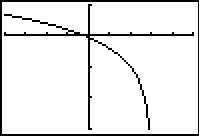
\includegraphics[width=2in]{./ExpLogsGraphics/Intro01.jpg} &

\hspace{1in} 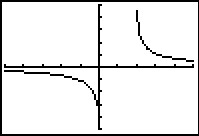
\includegraphics[width=2in]{./ExpLogsGraphics/Intro02.jpg} \\

$y = f(x) = 2\log(3-x)-1$ & 

\hspace{1in} $y = g(x) = \ln \left(\dfrac{x}{x-1}\right)$ \\

\end{tabular}

\end{center}

\vspace{-0.25in} \qed

\end{ex}

While logarithms have some interesting applications of their own which you'll explore in the exercises, their primary use to us will be to undo exponential functions. (This is, after all, how they were defined.)  Our last example solidifies this and reviews all of the material in the section.

\begin{ex}  Let $f(x) = 2^{x-1} - 3$. \label{proceduralinverse}

\begin{enumerate}

\item  Graph $f$ using transformations and state the domain and range of $f$.

\item  Explain why $f$ is invertible and find a formula for $f^{-1}(x)$.

\item  Graph $f^{-1}$ using transformations and state the domain and range of $f^{-1}$.

\item  Verify $\left(f^{-1} \circ f\right)(x) = x$ for all $x$ in the domain of $f$ and  $\left(f \circ f^{-1} \right)(x) = x$ for all $x$ in the domain of $f^{-1}$.

\item  Graph $f$ and $f^{-1}$ on the same set of axes and check the symmetry about the line $y = x$.

\end{enumerate}

{\bf Solution.}  

\begin{enumerate}

\item  If we identify $g(x) = 2^{x}$, we see $f(x) = g(x-1)-3$.  We pick the points $\left(-1, \frac{1}{2}\right)$, $(0,1)$ and $(1, 2)$ on the graph of $g$ along with the horizontal asymptote $y=0$ to track through the transformations. By Theorem \ref{transformationsthm} we first add $1$ to the $x$-coordinates of the points on the graph of $g$ (shifting $g$ to the right $1$ unit) to get $\left(0, \frac{1}{2}\right)$, $(1,1)$ and $(2, 2)$.  The horizontal asymptote remains $y=0$.  Next, we subtract $3$ from the $y$-coordinates, shifting the graph down $3$ units.  We get the points $\left(0, -\frac{5}{2}\right)$, $(1,-2)$ and $(2, -1)$ with the horizontal asymptote now at $y=-3$.  Connecting the dots in the order and manner as they were on the graph of $g$, we get the graph below.  We see that the domain of $f$ is the same as $g$, namely $(-\infty, \infty)$, but that the range of $f$ is $(-3, \infty)$.


\[\begin{array}{ccc}

\begin{mfpic}[10][8]{-4}{5}{-3.25}{8.25}
\point[2pt]{(-1,0.5), (0,1), (1,2)}
\axes
\tlabel[cc](5,-0.5){\scriptsize $x$}
\tlabel[cc](0.5,8.25){\scriptsize $y$}
\tcaption{\scriptsize $y = h(x) = 2^{x}$}
\xmarks{-3,-2,-1,1,2,3,4}
\ymarks{-3,-2,-1,1,2,3,4,5,6,7}
\tlpointsep{4pt}
\axislabels {x}{{\tiny $-3 \hspace{7pt}$} -3, {\tiny $-2 \hspace{7pt}$} -2, {\tiny $-1 \hspace{7pt}$} -1, {\tiny $1$} 1, {\tiny $2$} 2, {\tiny $3$} 3, {\tiny $4$} 4}
\axislabels {y}{{\tiny $-3$} -3, {\tiny $-2$} -2, {\tiny $-1$} -1,{\tiny $1$} 1, {\tiny $2$} 2, {\tiny $3$} 3, {\tiny $4$} 4, {\tiny $5$} 5, {\tiny $6$} 6, {\tiny $7$} 7}
\arrow \reverse \arrow \function{-3.5, 3, 0.1}{2**x}
\end{mfpic}

&

\xrightarrow{\hspace{1in}}

&

\begin{mfpic}[10][8]{-4}{5}{-3.25}{8.25}
\point[2pt]{(0,-2.5), (1,-2), (2,-1)}
\axes
\tlabel[cc](5,-0.5){\scriptsize $x$}
\tlabel[cc](0.5,8.25){\scriptsize $y$}
\tcaption{\scriptsize $y = f(x) = 2^{x-1}-3$}
\xmarks{-3,-2,-1,1,2,3,4}
\ymarks{-3,-2,-1,1,2,3,4,5,6,7}
\tlpointsep{4pt}
\axislabels {x}{{\tiny $-3 \hspace{7pt}$} -3, {\tiny $-2 \hspace{7pt}$} -2, {\tiny $-1 \hspace{7pt}$} -1, {\tiny $1$} 1, {\tiny $2$} 2, {\tiny $3$} 3, {\tiny $4$} 4}
\axislabels {y}{{\tiny $-2$} -2, {\tiny $-1$} -1,{\tiny $1$} 1, {\tiny $2$} 2, {\tiny $3$} 3, {\tiny $4$} 4, {\tiny $5$} 5, {\tiny $6$} 6, {\tiny $7$} 7}
\arrow \reverse \arrow \function{-2.5, 4, 0.1}{(2**(x-1))-3}
\dashed \polyline{(-4,-3),(5,-3)}
\end{mfpic} \\

\end{array}\]

\item  The graph of $f$ passes the Horizontal Line Test so $f$ is one-to-one, hence invertible.  To find a formula for $f^{-1}(x)$, we normally set $y=f(x)$, interchange the $x$ and $y$, then proceed to solve for $y$.  Doing so in this situation leads us to the equation $x = 2^{y-1}-3$.  We have yet to discuss how to solve this kind of equation, so we will attempt to find the formula for $f^{-1}$ from a procedural perspective.  If we break $f(x) = 2^{x-1}-3$ into a series of steps, we find $f$ takes an input $x$ and applies the steps

\begin{enumerate}

\item subtract $1$

\item put as an exponent on $2$

\item subtract $3$

\end{enumerate}

Clearly, to undo subtracting $1$, we will add $1$, and similarly we undo subtracting $3$ by adding $3$.  How do we undo the second step?  The answer is we use the logarithm.  By definition, $\log_{2}(x)$ undoes exponentiation by $2$.  Hence, $f^{-1}$ should

\begin{enumerate}

\item add $3$

\item take the logarithm base $2$

\item add $1$

\end{enumerate}

In symbols, $f^{-1}(x) = \log_{2}(x+3)+1$.  


\item  To graph $f^{-1}(x) = \log_{2}(x+3)+1$ using transformations, we start with $j(x) = \log_{2}(x)$.  We track the points $\left(\frac{1}{2},-1\right)$, $(1,0)$ and $(2, 1)$ on the graph of $j$ along with the vertical asymptote $x=0$ through the transformations using Theorem \ref{transformationsthm}.  Since $f^{-1}(x) = j(x+3)+1$, we first subtract $3$ from each of the $x$ values (including the vertical asymptote) to obtain  $\left(-\frac{5}{2},-1\right)$, $(-2,0)$ and $(-1, 1)$ with a vertical asymptote $x = -3$.  Next, we add $1$ to the $y$ values on the graph and get $\left(-\frac{5}{2},0\right)$, $(-2,1)$ and $(-1, 2)$.  If you are experiencing \textit{d\'{e}j\`{a} vu}, there is a good reason for it but we leave it to the reader to determine the source of this uncanny familiarity.  We obtain the graph below.  The domain of $f^{-1}$ is $(-3, \infty)$, which matches the range of $f$, and the range of $f^{-1}$ is $(-\infty, \infty)$, which matches the domain of $f$.

\[\begin{array}{ccc}

\begin{mfpic}[10]{-4}{9}{-4}{5}
\point[2pt]{(0.5,-1), (1,0), (2,1)}
\axes
\tlabel[cc](9,-0.5){\scriptsize $x$}
\tlabel[cc](0.5,5){\scriptsize $y$}
\tcaption{\scriptsize $y = j(x) = \log_{2}(x)$}
\ymarks{-3,-2,-1,1,2,3,4}
\xmarks{-3,-2,-1,1,2,3,4,5,6,7,8}
\tlpointsep{4pt}
\axislabels {y}{{\tiny $-3$} -3,{\tiny $-2$} -2, {\tiny $-1$} -1, {\tiny $1$} 1, {\tiny $2$} 2, {\tiny $3$} 3, {\tiny $4$} 4}
\axislabels {x}{{\tiny $-3 \hspace{7pt}$} -3, {\tiny $-2 \hspace{7pt}$} -2, {\tiny $-1 \hspace{7pt}$} -1,{\tiny $1$} 1, {\tiny $2$} 2, {\tiny $3$} 3, {\tiny $4$} 4, {\tiny $5$} 5, {\tiny $6$} 6, {\tiny $7$} 7, {\tiny $8$} 8}
\arrow \reverse \arrow \parafcn{-3.5, 3.1, 0.1}{(2**t,t)}
\end{mfpic}

&

\xrightarrow{\hspace{1in}}

&

\begin{mfpic}[10]{-4}{9}{-4}{5}
\point[2pt]{(-2.5,0), (-2,1), (-1,2)}
\axes
\tlabel[cc](9,-0.5){\scriptsize $x$}
\tlabel[cc](0.5,5){\scriptsize $y$}
\tcaption{\scriptsize $y = f^{-1}(x) = \log_{2}(x+3)+1$}
\ymarks{-3,-2,-1,1,2,3,4}
\xmarks{-3,-2,-1,1,2,3,4,5,6,7,8}
\tlpointsep{4pt}
\axislabels {y}{{\tiny $-3$} -3,{\tiny $-2$} -2, {\tiny $-1$} -1, {\tiny $1$} 1, {\tiny $2$} 2, {\tiny $3$} 3, {\tiny $4$} 4}
\axislabels {x}{{\tiny $-2 \hspace{7pt}$} -2, {\tiny $-1 \hspace{7pt}$} -1,{\tiny $1$} 1, {\tiny $2$} 2, {\tiny $3$} 3, {\tiny $4$} 4, {\tiny $5$} 5, {\tiny $6$} 6, {\tiny $7$} 7, {\tiny $8$} 8}
\arrow \reverse \arrow \parafcn{-2.5, 4.1, 0.1}{((2**(t-1))-3,t)}
\dashed \polyline{(-3,-4),(-3,5)}
\end{mfpic} \\

\end{array}\]

\item  We now verify that $f(x) = 2^{x-1}-3$ and $f^{-1}(x) = \log_{2}(x+3)+1$ satisfy the composition requirement for inverses.  For all real numbers $x$, 

\setlength{\extrarowheight}{4pt}

\[ \begin{array}{rclr}

\left(f^{-1}\circ f\right)(x) & = & f^{-1}(f(x)) & \\

& = & f^{-1}\left(2^{x-1}-3 \right) & \\

& = & \log_{2}\left( \left[2^{x-1}-3\right]+3 \right)+1 & \\

& = & \log_{2}\left( 2^{x-1} \right)+1 & \\

& = & (x-1) +1 & \mbox{ Since $\log_{2}\left(2^{u}\right) = u$ for all real numbers $u$} \\

& = & x \, \, \checkmark \\

\end{array} \]

\setlength{\extrarowheight}{2pt}

For all real numbers $x > -3$, we have\footnote{Pay attention - can you spot in which step below we need $x > -3$?} 

\setlength{\extrarowheight}{4pt}

\[ \begin{array}{rclr}

\left(f\circ f^{-1}\right)(x) & = & f\left(f^{-1}(x)\right) & \\

& = & f\left( \log_{2}(x+3)+1 \right) & \\

& = & 2^{\left( \log_{2}(x+3)+1 \right)-1} - 3 & \\

& = & 2^{\log_{2}(x+3)} - 3 & \\

& = & (x+3) -3 & \mbox{ Since $2^{\log_{2}(u)} = u$ for all real numbers $u > 0$} \\

& = & x \, \, \checkmark \\

\end{array} \]

\setlength{\extrarowheight}{2pt}

\item  Last, but certainly not least, we graph $y=f(x)$ and $y=f^{-1}(x)$ on the same set of axes and see the symmetry about the line $y=x$.

\begin{center}
\begin{mfpic}[12]{-4}{9}{-4}{9}
\axes
\tlabel[cc](9,-0.5){\scriptsize $x$}
\tlabel[cc](0.5,9){\scriptsize $y$}
\tlabel(-4,-5){$y = f(x) = 2^{x-1}-3$}
\tlabel(-4,-6){\mbox{\boldmath $y = f^{-1}(x) = \log_{2}(x+3)+1$}}
\xmarks{-3,-2,-1,1,2,3,4,5,6,7,8}
\ymarks{-3,-2,-1,1,2,3,4,5,6,7,8}
\tlpointsep{4pt}
\axislabels {x}{{\tiny $-3 \hspace{7pt}$} -3, {\tiny $-2 \hspace{7pt}$} -2, {\tiny $-1 \hspace{7pt}$} -1, {\tiny $1$} 1, {\tiny $2$} 2, {\tiny $3$} 3, {\tiny $4$} 4, {\tiny $5$} 5, {\tiny $6$} 6, {\tiny $7$} 7, {\tiny $8$} 8}
\axislabels {y}{{\tiny $-2$} -2, {\tiny $-1$} -1,{\tiny $1$} 1, {\tiny $2$} 2, {\tiny $3$} 3, {\tiny $4$} 4, {\tiny $5$} 5, {\tiny $6$} 6, {\tiny $7$} 7, {\tiny $8$} 8}
\arrow \reverse \arrow \function{-4.1, 4.1, 0.1}{(2**(x-1))-3}
\dashed \polyline{(-4,-3),(5,-3)}
\dashed \polyline{(-4,-4),(9,9)}
\dashed \polyline{(-3,-4),(-3,5)}
\penwd{1.5pt}
\arrow \reverse \arrow \parafcn{-4.1, 4.1, 0.1}{((2**(t-1))-3,t)}
\end{mfpic}

\end{center}
\end{enumerate}

\qed

\end{ex}

\newpage

\subsection{Exercises}

In Exercises \ref{rewritefirstex} - \ref{rewritelastex}, use the property: $b^{a} = c$ if and only if $\log_{b}(c) = a$ from Theorem \ref{logfcnprops} to rewrite the given equation in the other form.  That is, rewrite the exponential equations as logarithmic equations and rewrite the logarithmic equations as exponential equations.

\begin{multicols}{3}
\begin{enumerate}

\item  $2^{3} = 8$ \label{rewritefirstex}

\item  $5^{-3} = \frac{1}{125}$  

\item  $4^{5/2} = 32$  

\setcounter{HW}{\value{enumi}}
\end{enumerate}
\end{multicols}

\begin{multicols}{3}
\begin{enumerate}
\setcounter{enumi}{\value{HW}}

\item  $\left(\frac{1}{3}\right)^{-2} = 9$  

\item  $\left(\frac{4}{25}\right)^{-1/2} = \frac{5}{2}$  

\item  $10^{-3} = 0.001$ 

\setcounter{HW}{\value{enumi}}
\end{enumerate}
\end{multicols}

\begin{multicols}{3}
\begin{enumerate}
\setcounter{enumi}{\value{HW}}

\item  $e^{0}  = 1$  

\item  $\log_{5}(25) = 2$  

\item  $\log_{25} (5) = \frac{1}{2}$  

\setcounter{HW}{\value{enumi}}
\end{enumerate}
\end{multicols}

\begin{multicols}{3}
\begin{enumerate}
\setcounter{enumi}{\value{HW}}

\item  $\log_{3} \left(\frac{1}{81} \right) = -4$  

\item  $\log_{\frac{4}{3}} \left(\frac{3}{4} \right) = -1$  

\item  $\log(100) = 2$  

\setcounter{HW}{\value{enumi}}
\end{enumerate}
\end{multicols}

\begin{multicols}{3}
\begin{enumerate}
\setcounter{enumi}{\value{HW}}

\item  $\log (0.1) = -1$  

\item  $\ln(e) = 1$ 

\item  $\ln\left(\frac{1}{\sqrt{e}}\right) = -\frac{1}{2}$  \label{rewritelastex}

\setcounter{HW}{\value{enumi}}
\end{enumerate}
\end{multicols}

In Exercises \ref{simplifylogfirst} - \ref{simplifyloglast}, evaluate the expression.

\begin{multicols}{3}
\begin{enumerate}
\setcounter{enumi}{\value{HW}}

\item $\log_{3} (27)$  \label{simplifylogfirst}
\item $\log_{6} (216)$
\item $\log_{2} (32)$

\setcounter{HW}{\value{enumi}}
\end{enumerate}
\end{multicols}


\begin{multicols}{3}
\begin{enumerate}
\setcounter{enumi}{\value{HW}}

\item  $\log_{6} \left( \frac{1}{36} \right)$
\item $\log_{8} (4)$
\item $\log_{36} (216)$

\setcounter{HW}{\value{enumi}}
\end{enumerate}
\end{multicols}


\begin{multicols}{3}
\begin{enumerate}
\setcounter{enumi}{\value{HW}}

\item $\log_{\frac{1}{5}} (625)$
\item  $\log_{\frac{1}{6}} (216)$
\item $\log_{36} (36)$ 

\setcounter{HW}{\value{enumi}}
\end{enumerate}
\end{multicols}


\begin{multicols}{3}
\begin{enumerate}
\setcounter{enumi}{\value{HW}}

\item $\log \left(\frac{1}{1000000}\right)$
\item $\log(0.01)$
\item $\ln\left(e^3\right)$

\setcounter{HW}{\value{enumi}}
\end{enumerate}
\end{multicols}


\begin{multicols}{3}
\begin{enumerate}
\setcounter{enumi}{\value{HW}}

\item $\log_{4} (8)$
\item $\log_{6} (1)$
\item $\log_{13} \left(\sqrt{13}\right)$

\setcounter{HW}{\value{enumi}}
\end{enumerate}
\end{multicols}


\begin{multicols}{3}
\begin{enumerate}
\setcounter{enumi}{\value{HW}}

\item $\log_{36} \left(\sqrt[4]{36}\right)$
\item $7^{\log_{7} (3)}$
\item  $36^{\log_{36}(216)}$

\setcounter{HW}{\value{enumi}}
\end{enumerate}
\end{multicols}


\begin{multicols}{3}
\begin{enumerate}
\setcounter{enumi}{\value{HW}}

\item  $\log_{36} \left(36^{216}\right)$
\item $\ln \left(e^{5} \right)$
\item $\log \left(\sqrt[9]{10^{11}}\right)$

\setcounter{HW}{\value{enumi}}
\end{enumerate}
\end{multicols}


\begin{multicols}{3}
\begin{enumerate}
\setcounter{enumi}{\value{HW}}

\item  $\log\left( \sqrt[3]{10^5} \right)$
\item  $\ln \left( \frac{1}{\sqrt{e}}\right)$
\item $\log_{5} \left(3^{\log_{3} (5)}\right)$

\setcounter{HW}{\value{enumi}}
\end{enumerate}
\end{multicols}


\begin{multicols}{3}
\begin{enumerate}
\setcounter{enumi}{\value{HW}}

\item $\log\left(e^{\ln(100)}\right)$ 
\item $\log_{2}\left(3^{-\log_{3}(2)}\right)$
\item $\ln\left(42^{6\log(1)}\right)$ \label{simplifyloglast}

\setcounter{HW}{\value{enumi}}
\end{enumerate}
\end{multicols}

In Exercises \ref{domainlogfirst} - \ref{domainloglast}, find the domain of the function.

\begin{multicols}{2}
\begin{enumerate}
\setcounter{enumi}{\value{HW}}


\item $f(x) = \ln(x^{2} + 1)$ \label{domainlogfirst}
\item $f(x) = \log_{7}(4x + 8)$

\setcounter{HW}{\value{enumi}}
\end{enumerate}
\end{multicols}

\begin{multicols}{2}
\begin{enumerate}
\setcounter{enumi}{\value{HW}}


\item $f(x) = \ln(4x-20)$
\item $f(x) = \log \left(x^2+9x+18\right)$

\setcounter{HW}{\value{enumi}}
\end{enumerate}
\end{multicols}

\begin{multicols}{2}
\begin{enumerate}
\setcounter{enumi}{\value{HW}}

\item $f(x) = \log \left(\dfrac{x + 2}{x^{2} - 1}\right)$
\item $f(x) = \log\left(\dfrac{x^2+9x+18}{4x-20}\right)$

\setcounter{HW}{\value{enumi}}
\end{enumerate}
\end{multicols}

\begin{multicols}{2}
\begin{enumerate}
\setcounter{enumi}{\value{HW}}

\item $f(x) = \ln(7 - x) + \ln(x - 4)$
\item $f(x) = \ln(4x-20) + \ln\left(x^2+9x+18\right)$

\setcounter{HW}{\value{enumi}}
\end{enumerate}
\end{multicols}

\begin{multicols}{2}
\begin{enumerate}
\setcounter{enumi}{\value{HW}}

\item $f(x) = \log\left(x^2+x+1\right)$
\item $f(x) = \sqrt[4]{\log_{4} (x)}$

\setcounter{HW}{\value{enumi}}
\end{enumerate}
\end{multicols}

\begin{multicols}{2}
\begin{enumerate}
\setcounter{enumi}{\value{HW}}

\item $f(x) = \log_{9}(|x + 3| - 4)$
\item $f(x) = \ln(\sqrt{x - 4} - 3)$

\setcounter{HW}{\value{enumi}}
\end{enumerate}
\end{multicols}

\begin{multicols}{2}
\begin{enumerate}
\setcounter{enumi}{\value{HW}}

\item $f(x) = \dfrac{1}{3 - \log_{5} (x)}$
\item $f(x) = \dfrac{\sqrt{-1 - x}}{\log_{\frac{1}{2}} (x)}$

\setcounter{HW}{\value{enumi}}
\end{enumerate}
\end{multicols}

\begin{multicols}{2}
\begin{enumerate}
\setcounter{enumi}{\value{HW}}

\item $f(x) = \ln(-2x^{3} - x^{2} + 13x - 6)$  \label{domainloglast}

\setcounter{HW}{\value{enumi}}
\end{enumerate}
\end{multicols}

In Exercises \ref{graphexpfirst} - \ref{graphexplast}, sketch the graph of $y=g(x)$ by starting with the graph of $y = f(x)$ and using transformations.  Track at least three points of your choice and the horizontal asymptote through the transformations. State the domain and range of $g$.

\begin{multicols}{2}
\begin{enumerate}
\setcounter{enumi}{\value{HW}}


\item  $f(x) = 2^{x}$, $g(x) = 2^{x} - 1$ \label{graphexpfirst}

\item  $f(x) = \left(\frac{1}{3}\right)^{x}$, $g(x) = \left(\frac{1}{3}\right)^{x-1}$

\setcounter{HW}{\value{enumi}}
\end{enumerate}
\end{multicols}

\begin{multicols}{2}
\begin{enumerate}
\setcounter{enumi}{\value{HW}}

\item  $f(x) = 3^{x}$, $g(x) = 3^{-x}+2$

\item  $f(x) = 10^{x}$, $g(x) = 10^{\frac{x+1}{2}} - 20$  

\setcounter{HW}{\value{enumi}}
\end{enumerate}
\end{multicols}

\begin{multicols}{2}
\begin{enumerate}
\setcounter{enumi}{\value{HW}}

\item  $f(x) = e^{x}$, $g(x) = 8 - e^{-x}$

\item  $f(x) = e^{x}$, $g(x) = 10e^{-0.1x}$ \label{graphexplast}

\setcounter{HW}{\value{enumi}}
\end{enumerate}
\end{multicols}


In Exercises \ref{graphlogfirst} - \ref{graphloglast}, sketch the graph of $y=g(x)$ by starting with the graph of $y = f(x)$ and using transformations.  Track at least three points of your choice and the vertical asymptote through the transformations. State the domain and range of $g$.


\begin{multicols}{2}
\begin{enumerate}
\setcounter{enumi}{\value{HW}}

\item  $f(x) = \log_{2}(x)$, $g(x) = \log_{2}(x+1)$ \label{graphlogfirst}

\item  $f(x) = \log_{\frac{1}{3}}(x)$, $g(x) = \log_{\frac{1}{3}}(x)+1$

\setcounter{HW}{\value{enumi}}
\end{enumerate}
\end{multicols}

\begin{multicols}{2}
\begin{enumerate}
\setcounter{enumi}{\value{HW}}


\item  $f(x) = \log_{3}(x)$, $g(x) = -\log_{3}(x-2)$

\item  $f(x) = \log(x)$, $g(x) = 2\log(x+20) -1$  

\setcounter{HW}{\value{enumi}}
\end{enumerate}
\end{multicols}

\begin{multicols}{2}
\begin{enumerate}
\setcounter{enumi}{\value{HW}}


\item  $f(x) = \ln(x)$, $g(x) = -\ln(8-x)$

\item  $f(x) = \ln(x)$, $g(x) = -10\ln\left(\frac{x}{10}\right)$ \label{graphloglast}

\setcounter{HW}{\value{enumi}}
\end{enumerate}
\end{multicols}

\begin{enumerate}
\setcounter{enumi}{\value{HW}}

\smallskip

\item  Verify that each function in Exercises \ref{graphlogfirst} - \ref{graphloglast} is the inverse of the corresponding function in Exercises \ref{graphexpfirst} - \ref{graphexplast}.  (Match up \#\ref{graphexpfirst} and \#\ref{graphlogfirst}, and so on.)

\setcounter{HW}{\value{enumi}}
\end{enumerate}

In Exercises \ref{inverselogexpfirst} - \ref{inverselogexplast},  find the inverse of the function from the `procedural perspective' discussed in Example \ref{proceduralinverse} and graph the function and its inverse on the same set of axes.

\begin{multicols}{2}
\begin{enumerate}
\setcounter{enumi}{\value{HW}}

\item $f(x) = 3^{x + 2} - 4$  \label{inverselogexpfirst} 
\item $f(x) = \log_{4}(x - 1)$

\setcounter{HW}{\value{enumi}}
\end{enumerate}
\end{multicols}

\enlargethispage{.5in}
\vspace{-.2in}

\begin{multicols}{2}
\begin{enumerate}
\setcounter{enumi}{\value{HW}}

\item $f(x) = -2^{-x} + 1$
\item $f(x) = 5\log(x) - 2$ \label{inverselogexplast}

\setcounter{HW}{\value{enumi}}
\end{enumerate}
\end{multicols}
\vspace{-.2in}

\pagebreak

\phantomsection
\label{logarithmicscales}

(Logarithmic Scales) In Exercises \ref{Richterexercise} - \ref{pHexercise}, we introduce three widely used measurement scales which involve common logarithms: the Richter scale, the decibel scale and the pH scale.  The computations involved in all three scales are nearly identical so pay attention to the subtle differences. \index{logarithmic scales}

\begin{enumerate}
\setcounter{enumi}{\value{HW}}

\item \label{Richterexercise} \index{Richter Scale} \index{earthquake ! Richter Scale} Earthquakes are complicated events and it is not our intent to provide a complete discussion of the science involved in them.  Instead, we refer the interested reader to a solid course in Geology\footnote{Rock-solid, perhaps?} or the U.S. Geological Survey's Earthquake Hazards Program found \href{http://earthquake.usgs.gov/}{\underline{here}} and present only a simplified version of the \href{http://en.wikipedia.org/wiki/Richter_scale}{\underline{Richter scale}}.  The Richter scale measures the magnitude of an earthquake by comparing the amplitude of the seismic waves of the given earthquake to those of a ``magnitude 0 event'', which was chosen to be a seismograph reading of $0.001$ millimeters recorded on a seismometer 100 kilometers from the earthquake's epicenter.  Specifically, the magnitude of an earthquake is given by \[M(x) = \log \left(\dfrac{x}{0.001}\right)\] where $x$ is the seismograph reading in millimeters of the earthquake recorded 100 kilometers from the epicenter.  

\begin{enumerate}

\item Show that $M(0.001) = 0$.
\item Compute $M(80,000)$.
\item Show that an earthquake which registered 6.7 on the Richter scale had a seismograph reading ten times larger than one which measured 5.7.
\item Find two news stories about recent earthquakes which give their magnitudes on the Richter scale.  How many times larger was the seismograph reading of the earthquake with larger magnitude?

\end{enumerate}

\item \label{decibelexercise} \index{decibel} \index{sound intensity level ! decibel} While the decibel scale can be used in many disciplines,\footnote{See this  \href{http://en.wikipedia.org/wiki/Decibel}{\underline{webpage}} for more information.} we shall restrict our attention to its use in acoustics, specifically its use in measuring the intensity level of sound.\footnote{As of the writing of this exercise, the Wikipedia page given \href{http://en.wikipedia.org/wiki/Sound_intensity_level}{\underline{here}} states that it may not meet the ``general notability guideline'' nor does it cite any references or sources.  I find this odd because it is this very usage of the decibel scale which shows up in every College Algebra book I have read.  Perhaps those other books have been wrong all along and we're just blindly following tradition.}  The Sound Intensity Level $L$ (measured in decibels) of a sound intensity $I$ (measured in watts per square meter) is given by \[L(I) = 10\log\left( \dfrac{I}{10^{-12}} \right).\] Like the Richter scale, this scale compares $I$ to baseline: $10^{-12} \frac{W}{m^{2}}$ is the threshold of human hearing. 

\begin{enumerate}

\item Compute $L(10^{-6})$.
\item Damage to your hearing can start with short term exposure to sound levels around 115 decibels.  What intensity $I$ is needed to produce this level? 
\item Compute $L(1)$.  How does this compare with the threshold of pain which is around 140 decibels?

\end{enumerate}

\item \label{pHexercise} \index{pH} \index{acidity of a solution ! pH} \index{alkalinity of a solution ! pH} The pH of a solution is a measure of its acidity or alkalinity.  Specifically, $\mbox{pH} = -\log[\mbox{H}^{+}]$ where $[\mbox{H}^{+}]$ is the hydrogen ion concentration in moles per liter.  A solution with a pH less than 7 is an acid, one with a pH greater than 7 is a base (alkaline) and a pH of 7 is regarded as neutral.

\begin{enumerate}

\item The hydrogen ion concentration of pure water is $[\mbox{H}^{+}] = 10^{-7}$.  Find its pH.
\item Find the pH of a solution with $[\mbox{H}^{+}] = 6.3 \times 10^{-13}$.
\item The pH of gastric acid (the acid in your stomach) is about $0.7$.  What is the corresponding hydrogen ion concentration?

\end{enumerate}

\setcounter{HW}{\value{enumi}}
\end{enumerate}

\begin{enumerate}
\setcounter{enumi}{\value{HW}}

\item Show that $\log_{b} 1 = 0$ and $\log_{b} b = 1$ for every $b > 0, \; b \neq 1$.

\item (Crazy bonus question) Without using your calculator, determine which is larger: $e^{\pi}$ or $\pi^{e}$.

\setcounter{HW}{\value{enumi}}
\end{enumerate}


\newpage

\subsection{Answers}

\begin{multicols}{3}
\begin{enumerate}

\item $\log_{2}(8) = 3$

\item  $\log_{5}\left(\frac{1}{125}\right) = -3$

\item  $\log_{4}(32) = \frac{5}{2}$

\setcounter{HW}{\value{enumi}}
\end{enumerate}
\end{multicols}

\begin{multicols}{3}
\begin{enumerate}
\setcounter{enumi}{\value{HW}}


\item  $\log_{\frac{1}{3}}(9) = -2$

\item  $\log_{\frac{4}{25}}\left(\frac{5}{2}\right) = -\frac{1}{2}$

\item  $\log(0.001) = -3$

\setcounter{HW}{\value{enumi}}
\end{enumerate}
\end{multicols}

\begin{multicols}{3}
\begin{enumerate}
\setcounter{enumi}{\value{HW}}


\item  $\ln(1) = 0$

\item  $5^{2} = 25$

\item  $(25)^{\frac{1}{2}} = 5$

\setcounter{HW}{\value{enumi}}
\end{enumerate}
\end{multicols}

\begin{multicols}{3}
\begin{enumerate}
\setcounter{enumi}{\value{HW}}


\item  $3^{-4} = \frac{1}{81}$

\item  $\left(\frac{4}{3} \right)^{-1} = \frac{3}{4}$

\item  $10^{2} = 100$

\setcounter{HW}{\value{enumi}}
\end{enumerate}
\end{multicols}

\begin{multicols}{3}
\begin{enumerate}
\setcounter{enumi}{\value{HW}}


\item  $10^{-1} = 0.1$

\item  $e^{1} = e$

\item  $e^{-\frac{1}{2}} = \frac{1}{\sqrt{e}}$

\setcounter{HW}{\value{enumi}}
\end{enumerate}
\end{multicols}

\begin{multicols}{3}
\begin{enumerate}
\setcounter{enumi}{\value{HW}}

\item $\log_{3} (27) = 3$
\item $\log_{6} (216) = 3$
\item $\log_{2} (32) = 5$

\setcounter{HW}{\value{enumi}}
\end{enumerate}
\end{multicols}

\begin{multicols}{3}
\begin{enumerate}
\setcounter{enumi}{\value{HW}}


\item  $\log_{6} \left( \frac{1}{36} \right) = -2$
\item $\log_{8} (4) = \frac{2}{3}$
\item $\log_{36} (216) = \frac{3}{2}$

\setcounter{HW}{\value{enumi}}
\end{enumerate}
\end{multicols}

\begin{multicols}{3}
\begin{enumerate}
\setcounter{enumi}{\value{HW}}


\item $\log_{\frac{1}{5}} (625) = -4$
\item  $\log_{\frac{1}{6}} (216) = -3$
\item $\log_{36} (36)=1$ 

\setcounter{HW}{\value{enumi}}
\end{enumerate}
\end{multicols}

\begin{multicols}{3}
\begin{enumerate}
\setcounter{enumi}{\value{HW}}


\item $\log \frac{1}{1000000} = -6$
\item $\log(0.01) = -2$
\item $\ln\left(e^3\right) = 3$

\setcounter{HW}{\value{enumi}}
\end{enumerate}
\end{multicols}

\begin{multicols}{3}
\begin{enumerate}
\setcounter{enumi}{\value{HW}}


\item $\log_{4} (8) = \frac{3}{2}$
\item $\log_{6} (1) = 0$
\item $\log_{13} \left(\sqrt{13}\right) = \frac{1}{2}$

\setcounter{HW}{\value{enumi}}
\end{enumerate}
\end{multicols}

\begin{multicols}{3}
\begin{enumerate}
\setcounter{enumi}{\value{HW}}


\item $\log_{36} \left(\sqrt[4]{36}\right) = \frac{1}{4}$
\item $7^{\log_{7} (3)} = 3$
\item  $36^{\log_{36}(216)} = 216$

\setcounter{HW}{\value{enumi}}
\end{enumerate}
\end{multicols}

\begin{multicols}{3}
\begin{enumerate}
\setcounter{enumi}{\value{HW}}


\item  $\log_{36} \left(36^{216}\right) = 216$
\item $\ln(e^{5}) = 5$
\item $\log \left(\sqrt[9]{10^{11}}\right) = \frac{11}{9}$

\setcounter{HW}{\value{enumi}}
\end{enumerate}
\end{multicols}

\begin{multicols}{3}
\begin{enumerate}
\setcounter{enumi}{\value{HW}}


\item  $\log\left( \sqrt[3]{10^5} \right) = \frac{5}{3}$
\item  $\ln \left( \frac{1}{\sqrt{e}}\right) = -\frac{1}{2} $
\item $\log_{5} \left(3^{\log_{3} 5}\right) = 1$

\setcounter{HW}{\value{enumi}}
\end{enumerate}
\end{multicols}

\begin{multicols}{3}
\begin{enumerate}
\setcounter{enumi}{\value{HW}}


\item $\log\left(e^{\ln(100)}\right) = 2$
\item $\log_{2}\left(3^{-\log_{3}(2)}\right) = -1$
\item $\ln\left(42^{6\log(1)}\right) = 0$

\setcounter{HW}{\value{enumi}}
\end{enumerate}
\end{multicols}


\begin{multicols}{3}
\begin{enumerate}
\setcounter{enumi}{\value{HW}}


\item $(-\infty, \infty)$
\item $(-2, \infty)$
\item $(5, \infty)$

\setcounter{HW}{\value{enumi}}
\end{enumerate}
\end{multicols}


\begin{multicols}{3}
\begin{enumerate}
\setcounter{enumi}{\value{HW}}


\item $(-\infty, -6) \cup (-3, \infty)$
\item $(-2, -1) \cup (1, \infty)$
\item $(-6,-3) \cup (5, \infty)$

\setcounter{HW}{\value{enumi}}
\end{enumerate}
\end{multicols}


\begin{multicols}{3}
\begin{enumerate}
\setcounter{enumi}{\value{HW}}


\item $(4, 7)$
\item $(5, \infty)$
\item $(-\infty, \infty)$

\setcounter{HW}{\value{enumi}}
\end{enumerate}
\end{multicols}


\begin{multicols}{3}
\begin{enumerate}
\setcounter{enumi}{\value{HW}}


\item $[1, \infty)$
\item $(-\infty, -7) \cup (1, \infty)$
\item $(13, \infty)$

\setcounter{HW}{\value{enumi}}
\end{enumerate}
\end{multicols}


\begin{multicols}{3}
\begin{enumerate}
\setcounter{enumi}{\value{HW}}


\item $(0, 125) \cup (125, \infty)$
\item No domain
\item $(-\infty, -3) \cup \left(\frac{1}{2}, 2\right)$

\setcounter{HW}{\value{enumi}}
\end{enumerate}
\end{multicols}

\pagebreak

\begin{multicols}{2}
\begin{enumerate}
\setcounter{enumi}{\value{HW}}

\item  Domain of $g$:  $(-\infty, \infty)$\\
 Range of $g$:  $(-1, \infty)$\\
 
\begin{mfpic}[10]{-4}{4}{-2}{9}
\point[3pt]{(-1,-0.5), (0,0), (1,1)}
\axes
\tlabel[cc](4,-0.5){\scriptsize $x$}
\tlabel[cc](0.5,9){\scriptsize $y$}
\tcaption{\scriptsize $y = g(x) = 2^{x}-1$}
\xmarks{-3,-2,-1,1,2,3}
\ymarks{-1,1,2,3,4,5,6,7,8}
\tlabel[cc](-3,0.5){\tiny $-3 \hspace{7pt}$}
\tlabel[cc](-2,0.5){\tiny $-2 \hspace{7pt}$}
\tlabel[cc](-1,0.5){\tiny $-1 \hspace{7pt}$}
\tlabel[cc](2,-1.5){\tiny H.A. $y=-1$}
\tlpointsep{4pt}
\axislabels {x}{{\tiny $1$} 1, {\tiny $2$} 2, {\tiny $3$} 3}
\axislabels {y}{{\tiny $1$} 1, {\tiny $2$} 2, {\tiny $3$} 3, {\tiny $4$} 4, {\tiny $5$} 5, {\tiny $6$} 6, {\tiny $7$} 7, {\tiny $8$} 8}
\arrow \reverse \arrow \function{-3.5, 3.1, 0.1}{(2**(x))-1}
\dashed \polyline{(-4,-1),(4,-1)}
\end{mfpic}

\vfill

\columnbreak

\item  Domain of $g$:  $(-\infty, \infty)$ \\
 Range of $g$:  $(0, \infty)$ \\
 
\begin{mfpic}[10]{-4}{4}{-1}{10}
\point[3pt]{(0,3), (1,1), (2,0.3333)}
\axes
\tlabel[cc](4,-0.5){\scriptsize $x$}
\tlabel[cc](0.5,10){\scriptsize $y$}
\tcaption{\scriptsize $y = g(x) = \left(\frac{1}{3}\right)^{x-1}$}
\xmarks{-3,-2,-1,1,2,3}
\ymarks{1,2,3,4,5,6,7,8,9}
\tlpointsep{4pt}
\axislabels {x}{{\tiny $-3 \hspace{7pt}$} -3, {\tiny $-2 \hspace{7pt}$} -2, {\tiny $-1 \hspace{7pt}$} -1, {\tiny $1$} 1, {\tiny $2$} 2, {\tiny $3$} 3}
\axislabels {y}{{\tiny $1$} 1, {\tiny $2$} 2, {\tiny $3$} 3, {\tiny $4$} 4, {\tiny $5$} 5, {\tiny $6$} 6, {\tiny $7$} 7, {\tiny $8$} 8, {\tiny $9$} 9}
\arrow \reverse \arrow \function{-1.05, 3.5, 0.1}{3**(1-x)}
\end{mfpic} 

\setcounter{HW}{\value{enumi}}
\end{enumerate}
\end{multicols}

\begin{multicols}{2}
\begin{enumerate}
\setcounter{enumi}{\value{HW}}

\item  Domain of $g$:  $(-\infty, \infty)$\\
 Range of $g$:  $(2, \infty)$\\
 

\begin{mfpic}[10]{-4}{4}{-1}{12}
\point[3pt]{(1,2.3333), (0,3), (-1,5)}
\axes
\tlabel[cc](4,-0.5){\scriptsize $x$}
\tlabel[cc](0.5,12){\scriptsize $y$}
\tcaption{\scriptsize $y = g(x) = 3^{-x}+2$}
\xmarks{-3,-2,-1,1,2,3}
\ymarks{1,2,3,4,5,6,7,8,9,10,11}
\tlabel[cc](2,1){\tiny H.A. $y=2$}
\tlpointsep{4pt}
\axislabels {x}{{\tiny $-3 \hspace{7pt}$} -3, {\tiny $-2 \hspace{7pt}$} -2, {\tiny $-1 \hspace{7pt}$} -1, {\tiny $1$} 1, {\tiny $2$} 2, {\tiny $3$} 3}
\axislabels {y}{{\tiny $1$} 1, {\tiny $2$} 2, {\tiny $3$} 3, {\tiny $4$} 4, {\tiny $5$} 5, {\tiny $6$} 6, {\tiny $7$} 7, {\tiny $8$} 8, {\tiny $9$} 9, {\tiny $10$} 10, {\tiny $11$} 11}
\arrow \reverse \arrow \function{-2.05, 2.5, 0.1}{2+3**(0-x)}
\dashed \polyline{(-4,2),(4,2)}
\end{mfpic}

\vfill

\columnbreak

\item  Domain of $g$:  $(-\infty, \infty)$\\
 Range of $g$:  $(-20, \infty)$\\
 
\begin{mfpic}[10]{-3}{4}{-2}{9}
\point[3pt]{(-1,-1.9), (1,-1), (3,8)}
\axes
\tlabel[cc](4,-0.5){\scriptsize $x$}
\tlabel[cc](0.5,9){\scriptsize $y$}
\tcaption{\scriptsize $y = g(x) = 10^{\frac{x+1}{2}}-20$}
\xmarks{-3,-2,-1,1,2,3}
\ymarks{-2,-1,1,2,3,4,5,6,7,8}
\tlabel[cc](2,-2.5){\tiny H.A. $y=-20$}
\tlpointsep{4pt}
\axislabels {x}{{\tiny $-3 \hspace{7pt}$} -3, {\tiny $-2 \hspace{7pt}$} -2,  {\tiny $1$} 1, {\tiny $2$} 2, {\tiny $3$} 3}
\axislabels {y}{{\tiny $-10$} -1,{\tiny $10$} 1, {\tiny $20$} 2, {\tiny $30$} 3, {\tiny $40$} 4, {\tiny $50$} 5, {\tiny $60$} 6, {\tiny $70$} 7, {\tiny $80$} 8}
\arrow \reverse \arrow \function{-3, 3.06, 0.1}{((10**((x+1)/2))-20)/10}
\dashed \polyline{(-4,-2), (4,-2)}
\end{mfpic}

\setcounter{HW}{\value{enumi}}
\end{enumerate}
\end{multicols}

\begin{multicols}{2}
\begin{enumerate}
\setcounter{enumi}{\value{HW}}

\item  Domain of $g$:  $(-\infty, \infty)$\\
 Range of $g$:  $(-\infty, 8)$ \\
 
\begin{mfpic}[10]{-4}{4}{-1}{9}
\point[3pt]{(1,7.6321), (0,7), (-1,5.282)}
\axes
\tlabel[cc](4,-0.5){\scriptsize $x$}
\tlabel[cc](0.5,9){\scriptsize $y$}
\tlabel[cc](3,6){\tiny H.A. $y=8$}
\tcaption{\scriptsize $y = g(x) = 8-e^{-x}$}
\xmarks{-3,-2,-1,1,2,3}
\ymarks{1,2,3,4,5,6,7,8}
\tlpointsep{4pt}
\axislabels {x}{{\tiny $-3 \hspace{7pt}$} -3, {\tiny $-2 \hspace{7pt}$} -2, {\tiny $-1 \hspace{7pt}$} -1, {\tiny $1$} 1, {\tiny $2$} 2, {\tiny $3$} 3}
\axislabels {y}{{\tiny $1$} 1, {\tiny $2$} 2, {\tiny $3$} 3, {\tiny $4$} 4, {\tiny $5$} 5, {\tiny $6$} 6, {\tiny $7$} 7, {\tiny $8$} 8}
\arrow \reverse \arrow \function{-2.25, 2, 0.1}{8-exp(0-x)}
\dashed \polyline{(-4,8), (4,8)}
\end{mfpic}

\vfill

\columnbreak


\item  Domain of $g$:  $(-\infty, \infty)$\\
 Range of $g$:  $(0, \infty)$\\
 
\begin{mfpic}[10]{-4}{4}{-1}{9}
\point[3pt]{(1,0.3679), (0,1), (-1,2.718)}
\axes
\tlabel[cc](4,-0.5){\scriptsize $x$}
\tlabel[cc](0.5,9){\scriptsize $y$}
\tcaption{\scriptsize $y = g(x) = 10e^{-0.1x}$}
\xmarks{-3,-2,-1,1,2,3}
\ymarks{1,2,3,4,5,6,7,8}
\tlpointsep{4pt}
\axislabels {x}{{\tiny $-10 \hspace{7pt}$} -1, {\tiny $10$} 1, {\tiny $20$} 2, {\tiny $30$} 3}
\axislabels {y}{{\tiny $10$} 1, {\tiny $20$} 2, {\tiny $30$} 3, {\tiny $40$} 4, {\tiny $50$} 5, {\tiny $60$} 6, {\tiny $70$} 7, {\tiny $80$} 8}
\arrow \reverse \arrow \function{-2.15, 2, 0.1}{exp(0-x)}
\end{mfpic}

\setcounter{HW}{\value{enumi}}
\end{enumerate}
\end{multicols}

\begin{multicols}{2}
\begin{enumerate}
\setcounter{enumi}{\value{HW}}


\item  Domain of $g$: $(-1, \infty)$\\
 Range of $g$:  $(-\infty, \infty)$ \\

\begin{mfpic}[10]{-2}{9}{-4}{4}
\point[3pt]{(-0.5, -1), (0,0), (1,1)}
\axes
\tlabel[cc](0.5,4){\scriptsize $y$}
\tlabel[cc](9,-0.5){\scriptsize $x$}
\tlabel[cc](0.6, -3.1){\tiny $-3$}
\tlabel[cc](0.6, -2.1){\tiny $-2$}
\tlabel[cc](0.6, -1.1){\tiny $-1$}
\tcaption{\scriptsize $y = g(x) = \log_{2}(x+1)$}
\ymarks{-3,-2,-1,1,2,3}
\xmarks{-1,1,2,3,4,5,6,7,8}
\tlabel[cc](2,-4){\tiny V.A. $x=-1$}
\tlpointsep{4pt}
\axislabels {y}{{\tiny $1$} 1, {\tiny $2$} 2, {\tiny $3$} 3}
\axislabels {x}{{\tiny $1$} 1, {\tiny $2$} 2, {\tiny $3$} 3, {\tiny $4$} 4, {\tiny $5$} 5, {\tiny $6$} 6, {\tiny $7$} 7, {\tiny $8$} 8}
\arrow \reverse \arrow \parafcn{-3.5, 3.1, 0.1}{((2**(t))-1,t)}
\dashed \polyline{(-1,-3),(-1,4)}
\end{mfpic}

\vfill

\columnbreak

\item  Domain of $g$:  $(0, \infty)$\\
 Range of $g$:  $(-\infty, \infty)$ \\

\begin{mfpic}[10]{-1}{10}{-4}{4}
\point[3pt]{(3,0), (1,1), (0.3333,2)}
\axes
\tlabel[cc](0.5, 4){\scriptsize $y$}
\tlabel[cc](10,-0.5){\scriptsize $x$}
\tcaption{\scriptsize $y = g(x) = \log_{\frac{1}{3}}(x)+1$}
\ymarks{-3,-2,-1,1,2,3}
\xmarks{1,2,3,4,5,6,7,8,9}
\tlpointsep{4pt}
\axislabels {y}{{\tiny $-3$} -3, {\tiny $-2$} -2, {\tiny $-1$} -1, {\tiny $1$} 1, {\tiny $2$} 2, {\tiny $3$} 3}
\axislabels {x}{{\tiny $1$} 1, {\tiny $2$} 2, {\tiny $3$} 3, {\tiny $4$} 4, {\tiny $5$} 5, {\tiny $6$} 6, {\tiny $7$} 7, {\tiny $8$} 8, {\tiny $9$} 9}
\arrow \reverse \arrow \parafcn{-1.05, 3.5, 0.1}{(3**(1-t),t)}
\end{mfpic} 

\setcounter{HW}{\value{enumi}}
\end{enumerate}
\end{multicols}

\begin{multicols}{2}
\begin{enumerate}
\setcounter{enumi}{\value{HW}}


\item  Domain of $g$: $(2, \infty)$\\
 Range of $g$:  $(-\infty, \infty)$ \\
 
\begin{mfpic}[10]{-1}{12}{-4}{4}
\point[3pt]{(2.3333,1), (3,0), (5,-1)}
\axes
\tlabel[cc](0.5,4){\scriptsize $y$}
\tlabel[cc](12,-0.5){\scriptsize $x$}
\tcaption{\scriptsize $y = g(x) = -\log_{3}(x-2)$}
\ymarks{-3,-2,-1,1,2,3}
\xmarks{1,2,3,4,5,6,7,8,9,10,11}
\tlabel[cc](2,-4){\tiny V.A. $x=2$}
\tlpointsep{4pt}
\axislabels {y}{{\tiny $-3$} -3, {\tiny $-2$} -2, {\tiny $-1$} -1, {\tiny $1$} 1, {\tiny $2$} 2, {\tiny $3$} 3}
\axislabels {x}{{\tiny $1$} 1, {\tiny $2$} 2, {\tiny $3$} 3, {\tiny $4$} 4, {\tiny $5$} 5, {\tiny $6$} 6, {\tiny $7$} 7, {\tiny $8$} 8, {\tiny $9$} 9, {\tiny $10$} 10, {\tiny $11$} 11}
\arrow \reverse \arrow \parafcn{-2.05, 2.5, 0.1}{(2+3**(0-t),t)}
\dashed \polyline{(2,-3),(2,4)}
\end{mfpic} 

\vfill

\columnbreak




\item  Domain of $g$: $(-20, \infty)$\\
 Range of $g$:  $(-\infty, \infty)$\\

\begin{mfpic}[10]{-2}{11}{-3}{4}
\point[3pt]{(-1.9,-1), (-1,1), (8,3)}
\axes
\tlabel[cc](0.5,4){\scriptsize $y$}
\tlabel[cc](11,-0.5){\scriptsize $x$}
\tcaption{\scriptsize $y = g(x) = 2\log(x+20) -1$}
\ymarks{-3,-2,-1,1,2,3}
\xmarks{-2,-1,1,2,3,4,5,6,7,8,9,10}
\tlabel[cc](3,-3){\tiny V.A. $x=-20$}
\tlpointsep{4pt}
\axislabels {y}{{\tiny $-3$} -3, {\tiny $-2$} -2,  {\tiny $1$} 1, {\tiny $2$} 2, {\tiny $3$} 3}
\axislabels {x}{{\tiny $-10 \hspace{5pt}$} -1,{\tiny $10$} 1, {\tiny $20$} 2, {\tiny $30$} 3, {\tiny $40$} 4, {\tiny $50$} 5, {\tiny $60$} 6, {\tiny $70$} 7, {\tiny $80$} 8, {\tiny $90$} 9, {\tiny $100$} 10}
\arrow \reverse \arrow \parafcn{-3, 3.06, 0.1}{(((10**((t+1)/2))-20)/10,t)}
\dashed \polyline{(-2,-3), (-2,4)}
\end{mfpic}

\setcounter{HW}{\value{enumi}}
\end{enumerate}
\end{multicols}

\begin{multicols}{2}
\begin{enumerate}
\setcounter{enumi}{\value{HW}}


\item  Domain of $g$:  $(-\infty, 8)$\\
 Range of $g$:$(-\infty, \infty)$\\

\begin{mfpic}[10]{-1}{9}{-4}{4}
\point[3pt]{(7.6321,1), (7,0), (5.282,-1)}
\axes
\tlabel[cc](0.5,4){\scriptsize $y$}
\tlabel[cc](9,-0.5){\scriptsize $x$}
\tlabel[cc](4,-3){\tiny V.A. $x=8$}
\tcaption{\scriptsize $y = g(x) = -\ln(8-x)$}
\ymarks{-3,-2,-1,1,2,3}
\xmarks{1,2,3,4,5,6,7,8}
\tlpointsep{4pt}
\axislabels {y}{{\tiny $-3$} -3, {\tiny $-2$} -2, {\tiny $-1$} -1, {\tiny $1$} 1, {\tiny $2$} 2, {\tiny $3$} 3}
\axislabels {x}{{\tiny $1$} 1, {\tiny $2$} 2, {\tiny $3$} 3, {\tiny $4$} 4, {\tiny $5$} 5, {\tiny $6$} 6, {\tiny $7$} 7, {\tiny $8$} 8}
\arrow \reverse \arrow \parafcn{-2.25, 2, 0.1}{(8-exp(0-t),t)}
\dashed \polyline{(8,-3), (8,4)}
\end{mfpic} 

\vfill

\columnbreak

\item  Domain of $g$:  $(0, \infty)$\\
 Range of $g$:  $(-\infty, \infty)$\\

\begin{mfpic}[10]{-1}{9}{-4}{4}
\point[3pt]{(0.3679,1), (1,0), (2.718,-1)}
\axes
\tlabel[cc](0.5,4){\scriptsize $y$}
\tlabel[cc](9,-0.5){\scriptsize $x$}
\tcaption{\scriptsize $y = g(x) = -10\ln\left(\frac{x}{10}\right)$}
\ymarks{-3,-2,-1,1,2,3}
\xmarks{1,2,3,4,5,6,7,8}
\tlpointsep{4pt}
\axislabels {y}{{\tiny $-10$} -1, {\tiny $10$} 1, {\tiny $20$} 2, {\tiny $30$} 3}
\axislabels {x}{{\tiny $10$} 1, {\tiny $20$} 2, {\tiny $30$} 3, {\tiny $40$} 4, {\tiny $50$} 5, {\tiny $60$} 6, {\tiny $70$} 7, {\tiny $80$} 8}
\arrow \reverse \arrow \parafcn{-2.15, 2, 0.1}{(exp(0-t),t)}
\end{mfpic}

\setcounter{HW}{\value{enumi}}
\end{enumerate}
\end{multicols}

\pagebreak

\begin{multicols}{2}
\begin{enumerate}
\setcounter{enumi}{\value{HW}}
\addtocounter{enumi}{1}

\item $f(x) = 3^{x + 2} - 4$\\
$f^{-1}(x) = \log_{3}(x + 4) - 2$\\

\begin{mfpic}[10]{-5}{7}{-5}{7}
\axes
\tlabel[cc](7,-0.5){\scriptsize $x$}
\tlabel[cc](0.5,7){\scriptsize $y$}
\tlabel(-5,-6){\scriptsize $y = f(x) = 3^{x + 2} - 4$}
\tlabel(-5,-7){\scriptsize \mbox{\boldmath $y = f^{-1}(x) = \log_{3}(x + 4) - 2$}}
\xmarks{-4 step 1 until 6}
\ymarks{-4 step 1 until 6}
\tlpointsep{4pt}
\tiny
\axislabels {x}{{$-4 \hspace{7pt}$} -4, {$-3 \hspace{7pt}$} -3, {$-2 \hspace{7pt}$} -2, {$-1 \hspace{7pt}$} -1, {$1$} 1, {$2$} 2, {$3$} 3, {$4$} 4, {$5$} 5, {$6$} 6}
\axislabels {y}{{$-4$} -4, {$-3$} -3, {$-2$} -2, {$-1$} -1,{$1$} 1, {$2$} 2, {$3$} 3, {$4$} 4, {$5$} 5, {$6$} 6}
\normalsize
\arrow \reverse \arrow \function{-5, 0.15, 0.1}{(3**(x+2))-4}
\dashed \polyline{(-4,-5),(-4,7)}
\dashed \polyline{(-5,-5),(7,7)}
\dashed \polyline{(-5,-4),(7,-4)}
\penwd{1.5pt}
\arrow \reverse \arrow \function{-3.95, 7, 0.1}{(ln(x+4))/(ln(3.0)) - 2}
\end{mfpic}

\vfill

\columnbreak

\item $f(x) = \log_{4}(x - 1)$\\
$f^{-1}(x) = 4^{x} + 1$\\

\begin{mfpic}[13]{-3}{7}{-3}{7}
\axes
\tlabel[cc](7,-0.5){\scriptsize $x$}
\tlabel[cc](0.5,7){\scriptsize $y$}
\tlabel(-3,-4){\scriptsize $y = f(x) = \log_{4}(x - 1)$}
\tlabel(-3,-5){\scriptsize \mbox{\boldmath $y = f^{-1}(x) = 4^{x} + 1$}}
\xmarks{-2 step 1 until 6}
\ymarks{-2 step 1 until 6}
\tlpointsep{4pt}
\tiny
\axislabels {x}{{$-2 \hspace{7pt}$} -2, {$-1 \hspace{7pt}$} -1, {$1$} 1, {$2$} 2, {$3$} 3, {$4$} 4, {$5$} 5, {$6$} 6}
\axislabels {y}{{$-2$} -2, {$-1$} -1,{$1$} 1, {$2$} 2, {$3$} 3, {$4$} 4, {$5$} 5, {$6$} 6}
\normalsize
\arrow \reverse \arrow \function{1.03, 7, 0.1}{(ln(x-1))/(ln(4.0))}
\dashed \polyline{(-3,1),(7,1)}
\dashed \polyline{(1,7),(1,-3)}
\dashed \polyline{(-3,-3),(7,7)}
\penwd{1.5pt}
\arrow \reverse \arrow \function{-3, 1.25, 0.1}{(4**x) + 1}
\end{mfpic}

\setcounter{HW}{\value{enumi}}
\end{enumerate}
\end{multicols}


\begin{multicols}{2}
\begin{enumerate}
\setcounter{enumi}{\value{HW}}

\item $f(x) = -2^{-x} + 1$\\
$f^{-1}(x) = -\log_{2}(1 - x)$\\

\begin{mfpic}[17]{-3}{3}{-3}{3}
\axes
\tlabel[cc](3,-0.25){\scriptsize $x$}
\tlabel[cc](0.25,3){\scriptsize $y$}
\tlabel(-3,-3.5){\scriptsize $y = f(x) = -2^{-x} + 1$}
\tlabel(-3,-4){\scriptsize \mbox{\boldmath $y = f^{-1}(x) = -\log_{2}(1 - x)$}}
\xmarks{-2 step 1 until 2}
\ymarks{-2 step 1 until 2}
\tlpointsep{4pt}
\tiny
\axislabels {x}{{$-2 \hspace{7pt}$} -2, {$-1 \hspace{7pt}$} -1, {$1$} 1, {$2$} 2}
\axislabels {y}{{$-2$} -2, {$-1$} -1,{$1$} 1, {$2$} 2}
\normalsize
\arrow \reverse \arrow \function{-2, 3, 0.1}{1-(2**(-x))}
\dashed \polyline{(-3,1),(3,1)}
\dashed \polyline{(1,-3),(1,3)}
\dashed \polyline{(-3,-3),(3,3)}
\penwd{1.5pt}
\arrow \reverse \arrow \function{-3, 0.87, 0.1}{-(ln(1-x))/(ln(2.0))}
\end{mfpic}


\vfill

\columnbreak

\item $f(x) = 5\log(x) - 2$\\
$f^{-1}(x) = 10^{\frac{x + 2}{5}}$\\

\begin{mfpic}[10]{-5}{6}{-5}{6}
\axes
\tlabel[cc](6,-0.5){\scriptsize $x$}
\tlabel[cc](0.5,6){\scriptsize $y$}
\tlabel(-5,-6){\scriptsize $y = f(x) = 5\log(x) - 2$}
\tlabel(-5,-7.25){\scriptsize \mbox{\boldmath $y = f^{-1}(x) = 10^{\frac{x + 2}{5}}$}}
\xmarks{-4 step 1 until 5}
\ymarks{-4 step 1 until 5}
\tlpointsep{4pt}
\tiny
\axislabels {x}{{$-4 \hspace{7pt}$} -4, {$-3 \hspace{7pt}$} -3, {$-2 \hspace{7pt}$} -2, {$-1 \hspace{7pt}$} -1, {$1$} 1, {$2$} 2, {$3$} 3, {$4$} 4, {$5$} 5}
\axislabels {y}{{$-4$} -4, {$-3$} -3, {$-2$} -2, {$-1$} -1,{$1$} 1, {$2$} 2, {$3$} 3, {$4$} 4, {$5$} 5}
\normalsize
\arrow \reverse \arrow \function{0.3, 6, 0.1}{((5*ln(x))/ln(10.0)) - 2}
\dashed \polyline{(-5,-5),(6,6)}
\penwd{1.5pt}
\arrow \reverse \arrow \function{-5, 1.8, 0.1}{10**((x+2)/5)}
\end{mfpic}

\setcounter{HW}{\value{enumi}}
\end{enumerate}
\end{multicols}


\begin{enumerate}
\setcounter{enumi}{\value{HW}}


\item \begin{enumerate}

\item $M(0.001) = \log \left(\frac{0.001}{0.001} \right) = \log(1) = 0$.
\item $M(80,000) = \log \left(\frac{80,000}{0.001} \right) = \log(80,000,000) \approx 7.9$.

\end{enumerate}

\item \begin{enumerate}

\item $L(10^{-6}) = 60$ decibels.
\item $I = 10^{-.5} \approx 0.316$ watts per square meter.
\item Since $L(1) = 120$ decibels and $L(100) = 140$ decibels, a sound with intensity level 140 decibels has an intensity 100 times greater than a sound with intensity level 120 decibels.

\end{enumerate}

\item \begin{enumerate}

\item The pH of pure water is 7.
\item If $[\mbox{H}^{+}] = 6.3 \times 10^{-13}$ then the solution has a pH of 12.2.
\item $[\mbox{H}^{+}] = 10^{-0.7} \approx .1995$ moles per liter.

\end{enumerate}

\end{enumerate}

\closegraphsfile

\newpage

\section{Properties of Logarithms}

\mfpicnumber{1}

\opengraphsfile{LogProperties}

\setcounter{footnote}{0}

\label{LogProperties}

In Section \ref{IntroExpLogs}, we introduced the logarithmic functions as inverses of exponential functions and discussed a few of their functional properties from that perspective.  In this section, we explore the algebraic properties of logarithms.  Historically, these have played a huge role in the scientific development of our society since, among other things, they were used to develop analog computing devices called \href{http://en.wikipedia.org/wiki/Slide_rule}{\underline{slide rules}} which enabled scientists and engineers to perform accurate calculations leading to such things as space travel and the \href{http://www.redorbit.com/news/space/73297/nasa_marks_35th_anniversary_of_first_moon_landing/}{\underline{moon landing}}.  As we shall see shortly, logs inherit analogs of all of the properties of exponents you learned in Elementary and Intermediate Algebra.  We first extract two properties from Theorem \ref{logfcnprops} to remind us of the definition of a logarithm as the inverse of an exponential function.
\smallskip

\colorbox{ResultColor}{\bbm

\begin{thm}  \label{invpropslogs} \textbf{(Inverse Properties of Exponential and Log Functions)} Let $b > 0$, $b \neq 1$. \index{exponential function ! inverse properties of} \index{logarithm ! inverse properties of}

\vspace{-.25in}

\begin{itemize}

\item   $b^{a} = c$ if and only if $\log_{b}(c) = a$

\item  $\log_{b} \left(b^{x}\right) = x$ for all $x$ and $b^{\log_{b}(x)} = x$ for all $x > 0$

\end{itemize}

\end{thm}

\ebm}

\smallskip

Next, we spell out what it means for exponential and logarithmic functions to be one-to-one.

\smallskip

\colorbox{ResultColor}{\bbm

\begin{thm}  \label{explogsonetoone} \textbf{(One-to-one Properties of Exponential and Log Functions)} Let $f(x) = b^{x}$ and $g(x) = \log_{b}(x)$ where $b>0$, $b\neq 1$.  Then $f$ and $g$ are one-to-one.  In other words: \index{exponential function ! one-to-one properties of} \index{logarithm ! one-to-one properties of}

\begin{itemize}

\item  $b^{u} = b^{w}$ if and only if $u=w$ for all real numbers $u$ and $w$.

\item  $\log_{b}(u) = \log_{b}(w)$ if and only if $u=w$ for all real numbers $u > 0$, $w > 0$.

\end{itemize}

\end{thm}

\ebm}

\smallskip

We now state the algebraic properties of exponential functions which will serve as a basis for the properties of logarithms.  While these properties may look identical to the ones you learned in Elementary and Intermediate Algebra, they apply to real number exponents, not just rational exponents.  Note that in the theorem that follows, we are interested in the properties of exponential functions, so the base $b$ is restricted to $b > 0$, $b \neq 1$.  An added benefit of this restriction is that it eliminates the pathologies discussed in Section \ref{AlgebraicFunctions} when, for example, we simplified $\left(x^{2/3}\right)^{3/2}$ and obtained $|x|$ instead of what we had expected from the arithmetic in the exponents, $x^{1} = x$. 

\smallskip

\colorbox{ResultColor}{\bbm

\begin{thm}  \label{algpropexpfcns} \textbf{(Algebraic Properties of Exponential Functions)}  Let $f(x) = b^{x}$ be an exponential function ($b > 0$, $b\neq 1$) and let $u$ and $w$ be real numbers. \index{exponential function ! algebraic properties of}

\begin{itemize}

\item  \textbf{Product Rule:} \index{product rule ! for exponential functions} $f(u+w) = f(u) f(w)$.  In other words, $b^{u+w} = b^{u} b^{w}$

\item  \textbf{Quotient Rule:} \index{quotient rule ! for exponential functions} $f(u-w) = \dfrac{f(u)}{f(w)}$.  In other words, $b^{u-w} = \dfrac{b^{u}}{b^{w}}$

\item  \textbf{Power Rule:} \index{power rule ! for exponential functions} $\left(f(u)\right)^w = f(uw)$.  In other words, $\left(b^{u}\right)^{w} = b^{uw}$

\end{itemize}

\end{thm}

\ebm}

\smallskip

While the properties listed in Theorem \ref{algpropexpfcns} are certainly believable based on similar properties of integer and rational exponents, the full proofs require Calculus.  To each of these properties of exponential functions corresponds an analogous property of logarithmic functions.  We list these below in our next theorem.

\smallskip

\colorbox{ResultColor}{\bbm

\begin{thm}  \label{algproplogfcns} \textbf{(Algebraic Properties of Logarithm Functions)}  Let $g(x) =\log_{b}(x)$ be a logarithmic function ($b > 0$, $b\neq 1$) and let $u>0$ and $w>0$ be real numbers. \index{logarithm ! algebraic properties of}

\begin{itemize}

\item  \textbf{Product Rule:} \index{product rule ! for logarithms} $g(uw) = g(u)+ g(w)$.  In other words, $\log_{b}(uw) = \log_{b}(u) + \log_{b}(w)$

\item  \textbf{Quotient Rule:} \index{quotient rule ! for logarithms} $g\left(\dfrac{u}{w} \right) = g(u) - g(w)$.  In other words, $\log_{b} \left( \dfrac{u}{w} \right) = \log_{b}(u) - \log_{b}(w)$

\item  \textbf{Power Rule:} \index{power rule ! for logarithms} $g\left(u^{w}\right) =w g(u)$.  In other words, $\log_{b}\left(u^{w}\right) = w \log_{b}(u)$

\end{itemize}

\end{thm}

\ebm}

\smallskip

There are a couple of different ways to understand why Theorem \ref{algproplogfcns} is true.  Consider the product rule: $\log_{b}(uw) = \log_{b}(u) + \log_{b}(w)$.  Let $a = \log_{b}(uw)$, $c = \log_{b}(u)$, and $d = \log_{b}(w)$.  Then, by definition, $b^{a} = uw$, $b^{c} = u$ and $b^{d} = w$.  Hence, $b^{a} = uw = b^{c} b^{d} = b^{c+d}$, so that $b^{a} = b^{c+d}$.  By the one-to-one property of $b^{x}$, we have $a = c+d$. In other words, $\log_{b}(uw) = \log_{b}(u) + \log_{b}(w)$.  The remaining properties are proved similarly.  From a purely functional approach, we can see the properties in Theorem \ref{algproplogfcns} as an example of how inverse functions interchange the roles of inputs in outputs.  For instance, the Product Rule for exponential functions given in Theorem  \ref{algpropexpfcns}, $f(u+w) = f(u)f(w)$, says that adding inputs results in multiplying outputs.  Hence, whatever $f^{-1}$ is, it must take the products of outputs from $f$ and return them to the sum of their respective inputs.  Since the outputs from $f$ are the inputs to $f^{-1}$ and vice-versa, we have that that $f^{-1}$ must take products of its inputs to the sum of their respective outputs. This is precisely what the Product Rule for Logarithmic functions states in Theorem \ref{algproplogfcns}:  $g(uw) = g(u) + g(w)$.  The reader is encouraged to view the remaining properties listed in Theorem \ref{algproplogfcns} similarly.  The following examples help build familiarity with these properties.  In our first example, we are asked to `expand' the logarithms.  This means that we read the properties in Theorem \ref{algproplogfcns} from left to right and rewrite products inside the log as sums outside the log, quotients inside the log as  differences outside the log, and powers inside the log as factors outside the log.\footnote{Interestingly enough, it is the exact \textit{opposite} process (which we will practice later) that is most useful in Algebra, the utility of expanding logarithms becomes apparent in Calculus.}

\smallskip


\begin{ex}  \label{expandlogex} Expand the following using the properties of logarithms and simplify.  Assume when necessary that all quantities represent positive real numbers.

\begin{multicols}{3}
\begin{enumerate}

\item $\log_{2}\left(\dfrac{8}{x}\right)$

\item $\log_{0.1} \left(10 x^2 \right)$

\item  $\ln \left(\dfrac{3}{ex}\right)^2$

\setcounter{HW}{\value{enumi}}
\end{enumerate}
\end{multicols}

\begin{multicols}{3}
\begin{enumerate}
\setcounter{enumi}{\value{HW}}

\item  $\log \sqrt[3]{\dfrac{100 x^2}{yz^5}}$

\item  $\vphantom{\log \sqrt[3]{\dfrac{100 x^2}{yz^5}}} \log_{117}\left(x^2 - 4\right)$

\setcounter{HW}{\value{enumi}}
\end{enumerate}
\end{multicols}

{\bf Solution.}

\begin{enumerate}


\item  To expand $\log_{2}\left(\frac{8}{x}\right)$, we use the Quotient Rule identifying $u = 8$ and $w=x$ and simplify.

\setlength{\extrarowheight}{6pt}
\[ \begin{array}{rclr}

\log_{2}\left(\dfrac{8}{x}\right) & = &  \log_{2}(8) - \log_{2}(x) & \mbox{Quotient Rule} \\

& = &  3 - \log_{2}(x) & \mbox{Since $2^{3} = 8$} \\

& = & - \log_{2}(x) + 3 & \\

\end{array}\]

\setlength{\extrarowheight}{2pt}

\item   In the expression $\log_{0.1} \left(10 x^2 \right)$, we have a power (the $x^2$) and a product.  In order to use the Product Rule, the \textit{entire} quantity inside the logarithm must be raised to the same exponent.  Since the exponent $2$ applies only to the $x$, we first apply the Product Rule with $u=10$ and $w=x^2$.  Once we get the $x^2$ by itself inside the log, we may apply the Power Rule with $u=x$ and $w=2$ and simplify. 

\setlength{\extrarowheight}{6pt}
\[ \begin{array}{rclr}
\log_{0.1} \left(10 x^2 \right) & = &  \log_{0.1} (10) +  \log_{0.1} \left(x^2 \right) & \mbox{Product Rule} \\
                                & = &  \log_{0.1} (10)+ 2 \log_{0.1} (x) & \mbox{Power Rule} \\
                                & = &  -1 + 2 \log_{0.1} (x) & \mbox{Since $(0.1)^{-1} = 10$} \\
                                & = &  2 \log_{0.1} (x) - 1 & \\
                              
\end{array}\]
\setlength{\extrarowheight}{2pt}


\item  We have a power, quotient and product occurring in $\ln \left(\frac{3}{ex}\right)^2$.  Since the exponent $2$ applies to the entire quantity inside the logarithm, we begin with the Power Rule with $u=\frac{3}{ex}$ and $w = 2$.  Next, we see the Quotient Rule is applicable, with $u=3$ and $w=ex$, so we replace $\ln\left(\frac{3}{ex}\right)$  with the quantity $\ln(3) - \ln(ex)$. Since $\ln \left(\frac{3}{ex}\right)$ is being multiplied by $2$, the entire quantity $\ln(3) - \ln(ex)$ is multiplied by $2$.  Finally, we apply the Product Rule with $u=e$ and $w=x$, and replace $\ln(ex)$ with the quantity $\ln(e) + \ln(x)$, and simplify, keeping in mind that the natural log is log base $e$.

\setlength{\extrarowheight}{6pt}
\[ \begin{array}{rclr}

\ln \left(\dfrac{3}{ex}\right)^2 & = & 2 \ln \left(\dfrac{3}{ex}\right) & \mbox{Power Rule} \\
                                 & = & 2 \left[ \ln(3) - \ln(ex) \right] & \mbox{Quotient Rule} \\
                                 & = & 2 \ln(3) - 2\ln(ex) & \\
                                 & = & 2 \ln(3) - 2\left[\ln(e) + \ln(x)\right] & \mbox{Product Rule} \\
                                 & = & 2 \ln(3) - 2\ln(e) - 2 \ln(x) & \\
                                 & = & 2\ln(3) - 2 - 2 \ln(x) & \mbox{Since $e^{1} = e$} \\
                                 & = & - 2 \ln(x) + 2\ln(3) - 2 & \\
\end{array}\]
\setlength{\extrarowheight}{2pt}
                        

\item In Theorem \ref{algproplogfcns}, there is no mention of how to deal with radicals.  However, thinking back to Definition \ref{rationalexponentdefn}, we can rewrite the cube root as a $\frac{1}{3}$ exponent.  We begin by using the Power Rule\footnote{At this point in the text, the reader is encouraged to carefully read through each step and think of which quantity is playing the role of $u$ and which is playing the role of $w$ as we apply each property.}, and we keep in mind that the common log is log base $10$. 
\setlength{\extrarowheight}{6pt}
\[ \begin{array}{rclr}

\log \sqrt[3]{\dfrac{100 x^2}{yz^5}} & = & \log \left(\dfrac{100 x^2}{yz^5}\right)^{1/3} & \\ [10pt]
																		& = & \frac{1}{3} \log\left(\dfrac{100 x^2}{yz^5}\right) & \mbox{Power Rule} \\ [5pt]
																		& = & \frac{1}{3} \left[ \log\left(100x^2\right) - \log\left(yz^5\right) \right] & \mbox{Quotient Rule} \\ 
																		& = & \frac{1}{3}\log\left(100x^2\right) - \frac{1}{3}\log\left(yz^5\right) & \\
																		& = & \frac{1}{3}\left[ \log(100) + \log\left(x^2\right)\right] - \frac{1}{3} \left[ \log(y) + \log\left(z^5\right) \right] & \mbox{Product Rule} \\
																		& = & \frac{1}{3} \log(100) + \frac{1}{3} \log\left(x^2\right) - \frac{1}{3} \log(y) - \frac{1}{3} \log\left(z^5\right) \\
																		& = & \frac{1}{3} \log(100) + \frac{2}{3} \log(x) - \frac{1}{3} \log(y) - \frac{5}{3} \log(z) & \mbox{Power Rule} \\
																		& = & \frac{2}{3} + \frac{2}{3} \log(x) - \frac{1}{3} \log(y) - \frac{5}{3} \log(z) & \mbox{Since $10^2=100$} \\
																		& = &  \frac{2}{3} \log(x) - \frac{1}{3} \log(y) - \frac{5}{3} \log(z) + \frac{2}{3} & \\


\end{array} \]
\setlength{\extrarowheight}{2pt}

\item  At first it seems as if we have no means of simplifying $\log_{117}\left(x^2-4\right)$, since none of the properties of logs addresses the issue of expanding a difference \textit{inside} the logarithm.  However, we may factor $x^2 - 4 = (x+2)(x-2)$ thereby introducing a product which gives us license to use the Product Rule.

\setlength{\extrarowheight}{4pt}
\[ \begin{array}{rclr}

\log_{117}\left(x^2-4\right) & = & \log_{117} \left[(x+2)(x-2)\right] & \mbox{Factor} \\
														 & = & \log_{117}(x+2) + \log_{117}(x-2) & \mbox{Product Rule} \\
\end{array}\]
\setlength{\extrarowheight}{2pt}
\qed

\end{enumerate}

\end{ex}

A couple of remarks about Example \ref{expandlogex} are in order.  First, while not explicitly stated in the above example, a general rule of thumb to determine which log property to apply first to a complicated problem is `reverse order of operations.'  For example, if we were to substitute a number for $x$ into the expression $\log_{0.1} \left(10 x^2 \right)$, we would first square the $x$, then multiply by $10$.  The last step is the multiplication, which tells us the first log property to apply is the Product Rule.  In a multi-step problem, this rule can give the required guidance on which log property to apply at each step.  The reader is encouraged to look through the solutions to Example \ref{expandlogex} to see this rule in action.  Second, while we were instructed to assume when necessary that all quantities represented positive real numbers, the authors would be committing a sin of omission if we failed to point out that, for instance, the functions $f(x) = \log_{117}\left(x^2-4\right)$ and $g(x) = \log_{117}(x+2) + \log_{117}(x-2)$ have different domains, and, hence, are different functions. We leave it to the reader to verify the domain of $f$ is $(-\infty, -2) \cup (2,\infty)$ whereas the domain of $g$ is $(2,\infty)$.  In general, when using log properties to expand a logarithm, we may very well be restricting the domain as we do so.  One last comment before we move to reassembling logs from their various bits and pieces. The authors are well aware of the propensity for some students to become overexcited and invent their own properties of logs like $\log_{117}\left(x^2-4\right) = \log_{117}\left(x^2\right) - \log_{117}(4)$, which simply isn't true, in general.  The unwritten\footnote{The authors relish the irony involved in writing what follows.} property of logarithms is that if it isn't written in a textbook, it probably isn't true.    

\begin{ex}  \label{contractlogex} Use the properties of logarithms to write the following as a single logarithm.

\begin{multicols}{2}
\begin{enumerate}

\item  $\log_{3}(x-1) - \log_{3}(x+1)$

\item  $\log(x) + 2\log(y) - \log(z)$

\setcounter{HW}{\value{enumi}}
\end{enumerate}
\end{multicols}

\begin{multicols}{2}
\begin{enumerate}
\setcounter{enumi}{\value{HW}}

\item  $4\log_{2}(x) + 3$

\item  $-\ln(x) - \frac{1}{2}$


\end{enumerate}
\end{multicols}

{\bf Solution.} Whereas in Example \ref{expandlogex} we read the properties in Theorem \ref{algproplogfcns} from left to right to expand logarithms, in this example we read them from right to left.

\begin{enumerate}

\item The difference of logarithms requires the Quotient Rule: $\log_{3}(x-1) - \log_{3}(x+1) = \log_{3}\left(\frac{x-1}{x+1}\right)$.

\item  In the expression, $\log(x) + 2\log(y) - \log(z)$, we have both a sum and difference of logarithms.  However, before we use the product rule to combine $\log(x) + 2\log(y)$, we note that we need to somehow deal with the coefficient $2$ on $\log(y)$.  This can be handled using the Power Rule. We can then apply the Product and Quotient Rules as we move from left to right. Putting it all together, we have
\setlength{\extrarowheight}{6pt}
\[ \begin{array}{rclr}

\log(x) + 2\log(y) - \log(z) & = & \log(x) + \log\left(y^2\right) - \log(z) & \mbox{Power Rule} \\ [6pt]
                             & = & \log\left(xy^2\right) - \log(z) & \mbox{Product Rule} \\ [10pt]
                             & = & \log\left( \dfrac{xy^2}{z}\right) & \mbox{Quotient Rule} \\
                             
                            
\end{array}\]
\setlength{\extrarowheight}{2pt}

\item  We can certainly get started rewriting $4\log_{2}(x) + 3$ by applying the Power Rule to  $4\log_{2}(x)$ to obtain $\log_{2}\left(x^4\right)$, but in order to use the Product Rule to handle the addition, we need to rewrite $3$ as a logarithm base $2$.  From Theorem \ref{invpropslogs}, we know $3 = \log_{2}\left(2^3\right)$, so we get

\setlength{\extrarowheight}{4pt}
\[ \begin{array}{rclr}

4\log_{2}(x) + 3 & = & \log_{2}\left(x^4\right) + 3  & \mbox{Power Rule} \\ 
                             & = & \log_{2}\left(x^4\right) + \log_{2}\left(2^3\right)& \mbox{Since $3 = \log_{2}\left(2^3\right)$} \\
                             & = & \log_{2}\left(x^4\right) + \log_{2}(8)& \\
                             & = & \log_{2}\left( 8x^4\right) & \mbox{Product Rule} \\
                             
                            
\end{array}\]
\setlength{\extrarowheight}{2pt}

\item To get started with $-\ln(x) - \frac{1}{2}$, we rewrite  $-\ln(x)$ as $(-1) \ln(x)$.  We can then use the Power Rule to obtain $(-1)\ln(x) = \ln\left(x^{-1}\right)$. In order to use the Quotient Rule, we need to write $\frac{1}{2}$ as a natural logarithm. Theorem \ref{invpropslogs} gives us $\frac{1}{2} = \ln\left(e^{1/2}\right) = \ln\left(\sqrt{e}\right)$.  We have 

\setlength{\extrarowheight}{6pt}
\[ \begin{array}{rclr}

-\ln(x) - \frac{1}{2} & = & (-1)\ln(x) - \frac{1}{2}  &  \\ 
                             & = & \ln\left(x^{-1}\right) - \frac{1}{2} & \mbox{Power Rule} \\
                             & = & \ln\left(x^{-1}\right) - \ln\left(e^{1/2}\right)& \mbox{Since $\frac{1}{2} = \ln\left(e^{1/2}\right)$} \\
                             & = & \ln\left(x^{-1}\right) - \ln\left(\sqrt{e} \right)& \\ [6pt]
                             & = & \ln\left(\dfrac{x^{-1}}{\sqrt{e}}\right) & \mbox{Quotient Rule} \\ [10pt]
                             & = & \ln\left(\dfrac{1}{x\sqrt{e}}\right) &
\end{array}\]
\setlength{\extrarowheight}{2pt}

\end{enumerate}

\vspace{-.3in} \qed

\end{ex}

As we would expect, the rule of thumb for re-assembling logarithms is the opposite of what it was for dismantling them.  That is, if we are interested in rewriting an expression as a single logarithm, we apply log properties following the usual order of operations:  deal with multiples of logs first with the Power Rule, then deal with addition and subtraction using the Product and Quotient Rules, respectively. Additionally, we find that using log properties in this fashion can increase the domain of the expression.  For example, we leave it to the reader to verify the domain of $f(x) = \log_{3}(x-1) - \log_{3}(x+1)$ is $(1,\infty)$ but the domain of $g(x) = \log_{3}\left(\frac{x-1}{x+1}\right)$ is $(-\infty, -1) \cup (1, \infty)$.  We will need to keep this in mind when we solve equations involving logarithms in Section \ref{LogEquations} - it is precisely for this reason we will have to check for extraneous solutions.

\smallskip

The two logarithm buttons commonly found on calculators are the `LOG' and `LN' buttons which correspond to the common and natural logs, respectively.  Suppose we wanted an approximation to $\log_{2}(7)$.  The answer should be a little less than $3$, (Can you explain why?) but how do we coerce the calculator into telling us a more accurate answer?  We need the following theorem.

\smallskip

\colorbox{ResultColor}{\bbm

\begin{thm} \label{changeofbase} \textbf{(Change of Base Formulas)} Let $a,b >0$, $a,b \neq 1$. \index{change of base formulas} \index{exponential function ! change of base formula} \index{logarithm ! change of base formula}

\begin{itemize}

\item  $a^{x} = b^{x \log_{b}(a)}$ for all real numbers $x$.

\item  $\log_{a}(x) = \dfrac{\log_{b}(x)}{\log_{b}(a)}$ for all real numbers $x > 0$.

\end{itemize}

\end{thm}

\ebm}

\smallskip

The proofs of the Change of Base formulas are a result of the other properties studied in this section.  If we start with $b^{x \log_{b}(a)}$ and use the Power Rule in the exponent to rewrite $x \log_{b}(a)$ as $\log_{b}\left(a^{x}\right)$ and then apply one of the Inverse Properties in Theorem \ref{invpropslogs}, we get \[ b^{x \log_{b}(a)} = b^{\log_{b}\left(a^{x}\right)} = a^{x},\] as required.  To verify the logarithmic form of the property, we also use the Power Rule and an Inverse Property. We note that \[\log_{a}(x) \cdot \log_{b}(a) =  \log_{b} \left(a^{\log_{a}(x)}\right) = \log_{b}(x),\] and we get the result by dividing through by $\log_{b}(a)$.  Of course, the authors can't help but point out the inverse relationship between these two change of base formulas.  To change the base of an exponential expression, we \textit{multiply} the \textit{input} by the factor $\log_{b}(a)$.  To change the base of a logarithmic expression, we \textit{divide} the \textit{output} by the factor $\log_{b}(a)$.  While, in the grand scheme of things, both change of base formulas are really saying the same thing, the logarithmic form is the one usually encountered in Algebra while the exponential form isn't usually introduced until Calculus.\footnote{The authors feel so strongly about showing students that every property of logarithms comes from and corresponds to a property of exponents that we have broken tradition with the vast majority of other authors in this field.  This isn't the first time this happened, and it certainly won't be the last.} What Theorem \ref{changeofbase} really tells us is that all exponential and logarithmic functions are just scalings of one another.  Not only does this explain why their graphs have similar shapes, but it also tells us that we could do all of mathematics with a single base - be it $10$, $e$, $42$, or $117$.  Your Calculus teacher will have more to say about this when the time comes.

\begin{ex}  Use an appropriate change of base formula to convert the following expressions to ones with the indicated base.  Verify your answers using a calculator, as appropriate.
\begin{multicols}{2}
\begin{enumerate}

\item  $3^{2}$ to base $10$

\item  $2^{x}$ to base $e$

\setcounter{HW}{\value{enumi}}
\end{enumerate}
\end{multicols}

\begin{multicols}{2}
\begin{enumerate}
\setcounter{enumi}{\value{HW}}


\item $\log_{4}(5)$ to base $e$

\item $\ln(x)$ to base $10$

\end{enumerate}
\end{multicols}

{\bf Solution.}

\begin{enumerate}

\item  We apply the Change of Base formula with $a=3$ and $b=10$ to obtain $3^2 = 10^{2 \log(3)}$. Typing the latter in the calculator produces an answer of $9$ as required.

\item  Here, $a=2$ and $b = e$ so we have $2^{x} = e^{x \ln(2)}$.  To verify this on our calculator, we can graph $f(x) = 2^x$ and $g(x) = e^{x \ln(2)}$.  Their graphs are indistinguishable which provides evidence that they are the same function.

\begin{center}

\begin{tabular}{cc}

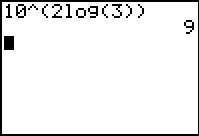
\includegraphics[width=2in]{./ExpLogsGraphics/LogProps01.jpg} &

\hspace{1in} 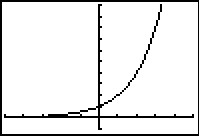
\includegraphics[width=2in]{./ExpLogsGraphics/LogProps02.jpg} \\

 & 

\hspace{1in} $y = f(x) = 2^x$ and $y = g(x) = e^{x \ln(2)}$ \\

\end{tabular}

\end{center}

\item  Applying the change of base with $a=4$ and $b=e$ leads us to write $\log_{4}(5) = \frac{\ln(5)}{\ln(4)}$.  Evaluating this in the calculator gives $\frac{\ln(5)}{\ln(4)} \approx 1.16$.  How do we check this really is the value of $\log_{4}(5)$?  By definition, $\log_{4}(5)$ is the exponent we put on $4$ to get $5$.  The calculator confirms this.\footnote{Which means if it is lying to us about the first answer it gave us, at least it is being consistent.}

\item  We write $\ln(x) = \log_{e}(x) = \frac{\log(x)}{\log(e)}$.  We graph both $f(x) = \ln(x)$ and $g(x) = \frac{\log(x)}{\log(e)}$ and find both graphs appear to be identical.

\begin{center}

\begin{tabular}{cc}

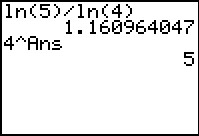
\includegraphics[width=2in]{./ExpLogsGraphics/LogProps03.jpg} &

\hspace{1in} 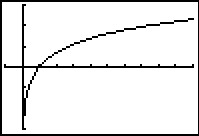
\includegraphics[width=2in]{./ExpLogsGraphics/LogProps04.jpg} \\

 & 

\hspace{1in} $y = f(x) = \ln(x)$ and $y = g(x) = \frac{\log(x)}{\log(e)}$ \\

\end{tabular}

\end{center}

\end{enumerate}

\vspace{-.25in} \qed

\end{ex}

\newpage

\subsection{Exercises}

In Exercises \ref{expandlogfirst} - \ref{expandloglast}, expand the given logarithm and simplify.  Assume when necessary that all quantities represent positive real numbers.

\begin{multicols}{3}
\begin{enumerate}

\item $\ln(x^{3}y^{2})$ \vphantom{$\log_{2}\left(\dfrac{128}{x^{2} + 4}\right)$} \label{expandlogfirst}
\item $\log_{2}\left(\dfrac{128}{x^{2} + 4}\right)$
\item $\log_{5}\left(\dfrac{z}{25}\right)^{3}$ \vphantom{$\log_{2}\left(\dfrac{128}{x^{2} + 4}\right)$}

\setcounter{HW}{\value{enumi}}
\end{enumerate}
\end{multicols}

\begin{multicols}{3}
\begin{enumerate}
\setcounter{enumi}{\value{HW}}

\item $\log(1.23 \times 10^{37})$ \vphantom{$\ln\left(\dfrac{\sqrt{z}}{xy}\right)$}
\item $\ln\left(\dfrac{\sqrt{z}}{xy}\right)$
\item $\log_{5} \left(x^2 - 25 \right)$ \vphantom{$\ln\left(\dfrac{\sqrt{z}}{xy}\right)$}

\setcounter{HW}{\value{enumi}}
\end{enumerate}
\end{multicols}

\begin{multicols}{3}
\begin{enumerate}
\setcounter{enumi}{\value{HW}}

\item $\log_{\sqrt{2}} \left(4x^3\right)$
\item $\log_{\frac{1}{3}}(9x(y^{3} - 8))$
\item $\log\left(1000x^3y^5\right)$

\setcounter{HW}{\value{enumi}}
\end{enumerate}
\end{multicols}

\begin{multicols}{3}
\begin{enumerate}
\setcounter{enumi}{\value{HW}}

\item $\log_{3} \left(\dfrac{x^2}{81y^4}\right)$
\item $\ln\left(\sqrt[4]{\dfrac{xy}{ez}}\right)$
\item $\log_{6} \left(\dfrac{216}{x^3y}\right)^4$

\setcounter{HW}{\value{enumi}}
\end{enumerate}
\end{multicols}

\begin{multicols}{3}
\begin{enumerate}
\setcounter{enumi}{\value{HW}}

\item $\log\left(\dfrac{100x\sqrt{y}}{\sqrt[3]{10}}\right)$ \vphantom{$\log_{\frac{1}{2}}\left(\dfrac{4\sqrt[3]{x^2}}{y\sqrt{z}}\right)$}
\item $\log_{\frac{1}{2}}\left(\dfrac{4\sqrt[3]{x^2}}{y\sqrt{z}}\right)$
\item $\ln \left(\dfrac{\sqrt[3]{x}}{10 \sqrt{yz}}\right)$ \vphantom{$\log_{\frac{1}{2}}\left(\dfrac{4\sqrt[3]{x^2}}{y\sqrt{z}}\right)$} \label{expandloglast}

\setcounter{HW}{\value{enumi}}
\end{enumerate}
\end{multicols}

In Exercises \ref{combinelogfirst} - \ref{combineloglast}, use the properties of logarithms to write the expression as a single logarithm.

\begin{multicols}{2}
\begin{enumerate}
\setcounter{enumi}{\value{HW}}

\item $4\ln(x) + 2\ln(y)$ \label{combinelogfirst}
\item $\log_{2}(x) + \log_{2}(y) - \log_{2}(z)$

\setcounter{HW}{\value{enumi}}
\end{enumerate}
\end{multicols}

\begin{multicols}{2}
\begin{enumerate}
\setcounter{enumi}{\value{HW}}

\item $\log_{3}(x) - 2 \log_{3}(y)$
\item $\frac{1}{2}\log_{3}(x) - 2\log_{3}(y) - \log_{3}(z)$

\setcounter{HW}{\value{enumi}}
\end{enumerate}
\end{multicols}

\begin{multicols}{2}
\begin{enumerate}
\setcounter{enumi}{\value{HW}}
\item $2 \ln(x) -3 \ln(y) - 4\ln(z)$
\item $\log(x) - \frac{1}{3} \log(z) + \frac{1}{2} \log(y)$

\setcounter{HW}{\value{enumi}}
\end{enumerate}
\end{multicols}

\begin{multicols}{2}
\begin{enumerate}
\setcounter{enumi}{\value{HW}}

\item $-\frac{1}{3} \ln(x) - \frac{1}{3}\ln(y) + \frac{1}{3} \ln(z)$
\item $\log_{5}(x) - 3$

\setcounter{HW}{\value{enumi}}
\end{enumerate}
\end{multicols}

\begin{multicols}{2}
\begin{enumerate}
\setcounter{enumi}{\value{HW}}

\item $3 - \log(x)$
\item $\log_{7}(x) + \log_{7}(x - 3) - 2$

\setcounter{HW}{\value{enumi}}
\end{enumerate}
\end{multicols}

\begin{multicols}{2}
\begin{enumerate}
\setcounter{enumi}{\value{HW}}

\item $\ln(x) + \frac{1}{2}$ 
\item $\log_{2}(x) + \log_{4}(x)$ 

\setcounter{HW}{\value{enumi}}
\end{enumerate}
\end{multicols}

\begin{multicols}{2}
\begin{enumerate}
\setcounter{enumi}{\value{HW}}

\item $\log_{2}(x) + \log_{4}(x-1)$
\item $\log_{2}(x) + \log_{\frac{1}{2}}(x - 1)$ \label{combineloglast}

\setcounter{HW}{\value{enumi}}
\end{enumerate}
\end{multicols}

\pagebreak

In Exercises \ref{changeofbasefirst} - \ref{changeofbaselast}, use the appropriate change of base formula to convert the given expression to an expression with the indicated base. 

\begin{multicols}{2}
\begin{enumerate}
\setcounter{enumi}{\value{HW}}

\item $7^{x - 1}$ to base $e$ \label{changeofbasefirst}
\item $\log_{3}(x + 2)$ to base 10

\setcounter{HW}{\value{enumi}}
\end{enumerate}
\end{multicols}

\begin{multicols}{2}
\begin{enumerate}
\setcounter{enumi}{\value{HW}}

\item $\left(\dfrac{2}{3}\right)^{x}$ to base $e$
\item $\log(x^{2} + 1)$ to base $e$ \vphantom{$\left(\dfrac{2}{3}\right)^{x}$}\label{changeofbaselast}

\setcounter{HW}{\value{enumi}}
\end{enumerate}
\end{multicols}

In Exercises \ref{changeofbaseapproxfirst} - \ref{changeofbaseapproxlast}, use the appropriate change of base formula to approximate the logarithm.

\begin{multicols}{3}
\begin{enumerate}
\setcounter{enumi}{\value{HW}}

\item $\log_{3}(12)$ \label{changeofbaseapproxfirst}
\item $\log_{5}(80)$
\item $\log_{6}(72)$

\setcounter{HW}{\value{enumi}}
\end{enumerate}
\end{multicols}

\begin{multicols}{3}
\begin{enumerate}
\setcounter{enumi}{\value{HW}}

\item $\log_{4}\left(\dfrac{1}{10}\right)$
\item $\log_{\frac{3}{5}}(1000)$ \vphantom{$\log_{4}\left(\dfrac{1}{10}\right)$}
\item $\log_{\frac{2}{3}}(50)$ \vphantom{$\log_{4}\left(\dfrac{1}{10}\right)$} \label{changeofbaseapproxlast}

\setcounter{HW}{\value{enumi}}
\end{enumerate}
\end{multicols}

\begin{enumerate}
\setcounter{enumi}{\value{HW}}

\item Compare and contrast the graphs of $y = \ln(x^{2})$ and $y = 2\ln(x)$.

\item Prove the Quotient Rule and Power Rule for Logarithms.

\item Give numerical examples to show that, in general,

\begin{enumerate}

\item $\log_{b}(x + y) \neq \log_{b}(x) + \log_{b}(y)$
\item $\log_{b}(x - y) \neq \log_{b}(x) - \log_{b}(y)$
\item $\log_{b}\left(\dfrac{x}{y}\right) \neq \dfrac{\log_{b}(x)}{\log_{b}(y)}$

\end{enumerate}

\item \label{HendersonHasselbalch} \index{Henderson-Hasselbalch Equation} The Henderson-Hasselbalch Equation:  Suppose $HA$ represents a weak acid. Then we have a reversible chemical reaction 
\[HA \rightleftharpoons H^{+} + A^{-}.\]  
The acid disassociation constant, $K_{a}$, is given by 
\[K_{\alpha} = \frac{[H^{+}][A^{-}]}{[HA]} = [H^{+}]\frac{[A^{-}]}{[HA]},\]
where the square brackets denote the concentrations just as they did in Exercise \ref{pHexercise} in Section \ref{IntroExpLogs}.  The symbol p$K_{a}$ is defined similarly to pH in that p$K_{a} = -\log(K_{a})$.  Using the definition of pH from Exercise \ref{pHexercise} and the properties of logarithms, derive the Henderson-Hasselbalch Equation which states 
\[\mbox{pH} = \mbox{p}K_{a} + \log\dfrac{[A^{-}]}{[HA]}\]

\item Research the history of logarithms including the origin of the word `logarithm' itself.  Why is the abbreviation of natural log `ln' and not `nl'?

\item There is a scene in the movie `Apollo 13' in which several people at Mission Control use slide rules to verify a computation.  Was that scene accurate?  Look for other pop culture references to logarithms and slide rules.

\end{enumerate}

\newpage

\subsection{Answers}


\begin{multicols}{2}
\begin{enumerate}

\item $3\ln(x) + 2\ln(y)$
\item $7 - \log_{2}(x^{2} + 4)$

\setcounter{HW}{\value{enumi}}
\end{enumerate}
\end{multicols}

\begin{multicols}{2}
\begin{enumerate}
\setcounter{enumi}{\value{HW}}


\item $3\log_{5}(z) - 6$
\item $\log(1.23) + 37$

\setcounter{HW}{\value{enumi}}
\end{enumerate}
\end{multicols}

\begin{multicols}{2}
\begin{enumerate}
\setcounter{enumi}{\value{HW}}

\item $\frac{1}{2}\ln(z) - \ln(x) - \ln(y)$
\item  $\log_{5}(x-5) + \log_{5}(x+5)$

\setcounter{HW}{\value{enumi}}
\end{enumerate}
\end{multicols}

\begin{multicols}{2}
\begin{enumerate}
\setcounter{enumi}{\value{HW}}

\item  $3\log_{\sqrt{2}}(x) + 4$
\item \small$-2 + \log_{\frac{1}{3}}(x) + \log_{\frac{1}{3}}(y - 2) + \log_{\frac{1}{3}}(y^{2} + 2y + 4)$\normalsize

\setcounter{HW}{\value{enumi}}
\end{enumerate}
\end{multicols}

\begin{multicols}{2}
\begin{enumerate}
\setcounter{enumi}{\value{HW}}

\item $3 + 3\log(x) + 5 \log(y)$
\item $2\log_{3}(x) - 4 - 4\log_{3}(y)$

\setcounter{HW}{\value{enumi}}
\end{enumerate}
\end{multicols}

\begin{multicols}{2}
\begin{enumerate}
\setcounter{enumi}{\value{HW}}

\item $\frac{1}{4} \ln(x) + \frac{1}{4} \ln(y) - \frac{1}{4} - \frac{1}{4} \ln(z)$
\item $12-12\log_{6}(x) - 4\log_{6}(y)$

\setcounter{HW}{\value{enumi}}
\end{enumerate}
\end{multicols}

\begin{multicols}{2}
\begin{enumerate}
\setcounter{enumi}{\value{HW}}

\item $\frac{5}{3}+\log(x)+\frac{1}{2}\log(y)$
\item $-2+\frac{2}{3}\log_{\frac{1}{2}}(x)-\log_{\frac{1}{2}}(y)-\frac{1}{2}\log_{\frac{1}{2}}(z)$

\setcounter{HW}{\value{enumi}}
\end{enumerate}
\end{multicols}

\begin{multicols}{2}
\begin{enumerate}
\setcounter{enumi}{\value{HW}}

\item $\frac{1}{3} \ln(x) - \ln(10) - \frac{1}{2}\ln(y)-\frac{1}{2}\ln(z)$
\item $\ln(x^{4}y^{2})$
\setcounter{HW}{\value{enumi}}
\end{enumerate}
\end{multicols}

\begin{multicols}{3}
\begin{enumerate}
\setcounter{enumi}{\value{HW}}

\item $\log_{2}\left(\frac{xy}{z}\right)$
\item $\log_{3} \left( \frac{x}{y^2} \right)$
\item $\log_{3}\left(\frac{\sqrt{x}}{y^{2}z}\right)$

\setcounter{HW}{\value{enumi}}
\end{enumerate}
\end{multicols}

\begin{multicols}{3}
\begin{enumerate}
\setcounter{enumi}{\value{HW}}


\item $\ln\left( \frac{x^2}{y^3z^4} \right)$
\item $\log\left(\frac{x \sqrt{y}}{\sqrt[3]{z}}  \right)$
\item $\ln\left(\sqrt[3]{\frac{z}{xy}}   \right)$

\setcounter{HW}{\value{enumi}}
\end{enumerate}
\end{multicols}

\begin{multicols}{3}
\begin{enumerate}
\setcounter{enumi}{\value{HW}}

\item $\log_{5}\left(\frac{x}{125}\right)$
\item $\log\left(\frac{1000}{x}\right)$
\item $\log_{7}\left(\frac{x(x - 3)}{49}\right)$

\setcounter{HW}{\value{enumi}}
\end{enumerate}
\end{multicols}

\begin{multicols}{3}
\begin{enumerate}
\setcounter{enumi}{\value{HW}}

\item $\ln \left(x \sqrt{e} \right)$
\item $\log_{2}\left(x^{3/2}\right)$
\item $\log_{2}\left(x \sqrt{x-1}\right)$


\setcounter{HW}{\value{enumi}}
\end{enumerate}
\end{multicols}


\begin{multicols}{3}
\begin{enumerate}
\setcounter{enumi}{\value{HW}}
\item $\vphantom{\frac{\log(x + 2)}{\log(3)}}\log_{2}\left(\frac{x}{x - 1}\right)$ 
\item $\vphantom{\frac{\log(x + 2)}{\log(3)}}7^{x - 1} = e^{(x - 1)\ln(7)}$
\item $\log_{3}(x + 2) = \frac{\log(x + 2)}{\log(3)}$


\setcounter{HW}{\value{enumi}}
\end{enumerate}
\end{multicols}


\begin{multicols}{2}
\begin{enumerate}
\setcounter{enumi}{\value{HW}}

\item $\left(\frac{2}{3}\right)^{x} = e^{x\ln(\frac{2}{3})}$
\item $\log(x^{2} + 1) = \frac{\ln(x^{2} + 1)}{\ln(10)}$

\setcounter{HW}{\value{enumi}}
\end{enumerate}
\end{multicols}

\begin{multicols}{2}
\begin{enumerate}
\setcounter{enumi}{\value{HW}}

\item $\log_{3}(12) \approx 2.26186$
\item $\log_{5}(80) \approx 2.72271$

\setcounter{HW}{\value{enumi}}
\end{enumerate}
\end{multicols}

\begin{multicols}{2}
\begin{enumerate}
\setcounter{enumi}{\value{HW}}

\item $\log_{6}(72) \approx 2.38685$
\item $\log_{4}\left(\frac{1}{10}\right) \approx -1.66096$

\setcounter{HW}{\value{enumi}}
\end{enumerate}
\end{multicols}

\begin{multicols}{2}
\begin{enumerate}
\setcounter{enumi}{\value{HW}}
\item $\log_{\frac{3}{5}}(1000) \approx -13.52273$
\item $\log_{\frac{2}{3}}(50) \approx -9.64824$

\setcounter{HW}{\value{enumi}}
\end{enumerate}
\end{multicols}

\closegraphsfile

\newpage

\section{Exponential Equations and Inequalities}

\mfpicnumber{1}

\opengraphsfile{ExpEquations}

\setcounter{footnote}{0}

\label{ExpEquations}

In this section we will develop techniques for solving equations involving exponential functions.  Suppose, for instance,  we wanted to solve the equation $2^{x} = 128$.  After a moment's calculation, we find $128 = 2^{7}$, so we have $2^{x} = 2^{7}$.  The one-to-one property of exponential functions, detailed in Theorem \ref{explogsonetoone}, tells us that $2^{x} = 2^{7}$ if and only if $x=7$.  This means that not only is $x=7$ a solution to $2^{x} = 2^{7}$, it is the \textit{only} solution.  Now suppose we change the problem ever so slightly to $2^{x} = 129$.  We could use one of the inverse properties of exponentials and logarithms listed in Theorem \ref{invpropslogs} to write $129 = 2^{\log_{2}(129)}$.  We'd then have $2^{x} = 2^{\log_{2}(129)}$, which means our solution is $x = \log_{2}(129)$. This makes sense because, after all, the definition of $\log_{2}(129)$ is `the exponent we put on $2$ to get $129$.' Indeed we could have obtained this solution directly by rewriting the equation $2^{x} = 129$ in its logarithmic form $\log_{2}(129) = x$.  Either way, in order to get a reasonable decimal approximation to this number, we'd use the change of base formula, Theorem \ref{changeofbase}, to give us something more calculator friendly,\footnote{You can use natural logs or common logs.  We choose natural logs.  (In Calculus, you'll learn these are the most `mathy' of the logarithms.)} say $\log_{2}(129) = \frac{\ln(129)}{\ln(2)}$.  Another way to arrive at this answer is as follows


\[ \begin{array}{rclr}
2^{x} & = & 129 & \\
\ln\left(2^{x}\right) & = & \ln(129) & \mbox{Take the natural log of both sides.} \\
x \ln(2) & = & \ln(129) & \mbox{Power Rule} \\ [4pt]
x & = &\dfrac{\ln(129)}{\ln(2)} & \\
\end{array}\]

`Taking the natural log' of both sides is akin to squaring both sides: since $f(x) = \ln(x)$ is a \textit{function}, as long as two quantities are equal, their natural logs are equal.\footnote{This is also the `if' part of the statement $\log_{b}(u) = \log_{b}(w)$ if and only if $u=w$ in Theorem \ref{explogsonetoone}.} Also note that we treat $\ln(2)$ as any other non-zero real number and divide it through\footnote{Please resist the temptation to divide both sides by `$\ln$' instead of $\ln(2)$.   Just like it wouldn't make sense to divide both sides by the square root symbol `$\sqrt{\vphantom{2} \,}$' when solving $x \sqrt{2} = 5$, it makes no sense to divide by `$\ln$'.}  to isolate the variable $x$.  We summarize below the two common ways to solve exponential equations, motivated by our examples.

\smallskip

\colorbox{ResultColor}{\bbm

\centerline{\textbf{Steps for Solving an Equation involving Exponential Functions}} \index{exponential function ! solving equations with}

\begin{enumerate}

\item  Isolate the exponential function.

\item  

\begin{enumerate}

\item  If convenient, express both sides with a common base and equate the exponents.

\item  Otherwise, take the natural log of both sides of the equation and use the Power Rule.


\end{enumerate}


\end{enumerate}

\ebm}

\smallskip


\begin{ex}  \label{expeqnsex1} Solve the following equations.  Check your answer graphically using a calculator.

\begin{multicols}{3}
\begin{enumerate}

\item  $2^{3x} = 16^{1-x}$

\item  $2000 = 1000 \cdot 3^{-0.1 t}$ 

\item  $9 \cdot 3^{x} = 7^{2x}$

\setcounter{HW}{\value{enumi}}
\end{enumerate}
\end{multicols}

\begin{multicols}{3}
\begin{enumerate}
\setcounter{enumi}{\value{HW}}

\item  $75 = \frac{100}{1 + 3e^{-2t}}$

\item  $25^{x} = 5^{x} + 6$

\item  $\frac{e^{x} - e^{-x}}{2} = 5$

\end{enumerate}
\end{multicols}

{\bf Solution.}

\begin{enumerate}

\item  Since $16$ is a power of $2$, we can rewrite  $2^{3x} =  16^{1-x}$ as $2^{3x} = \left(2^4\right)^{1-x}$.  Using properties of exponents, we get $2^{3x} = 2^{4(1-x)}$.  Using the one-to-one property of exponential functions, we get $3x = 4(1-x)$ which gives $x=\frac{4}{7}$. To check graphically, we set $f(x) = 2^{3x}$ and $g(x) = 16^{1-x}$ and see that they intersect at $x=\frac{4}{7} \approx 0.5714$.

\item  We begin solving $2000 = 1000 \cdot 3^{-0.1 t}$  by dividing both sides by $1000$ to isolate the exponential which yields $3^{-0.1t} = 2$.  Since it is inconvenient to write $2$ as a power of $3$, we use the natural log to get $\ln\left(3^{-0.1t}\right) = \ln(2)$.  Using the Power Rule, we get $-0.1 t \ln(3) = \ln(2)$, so we divide both sides by $-0.1 \ln(3)$ to get $t = -\frac{\ln(2)}{0.1 \ln(3)} = -\frac{10\ln(2)}{\ln(3)}$.  On the calculator, we graph $f(x) = 2000$ and $g(x) =  1000 \cdot 3^{-0.1 x}$ and find that they intersect at $x = -\frac{10\ln(2)}{\ln(3)} \approx -6.3093$.

\begin{center}

\begin{tabular}{cc}

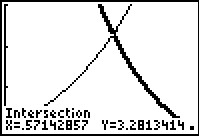
\includegraphics[width=2in]{./ExpLogsGraphics/ExpEqns01.jpg} &

\hspace{0.75in} 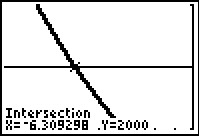
\includegraphics[width=2in]{./ExpLogsGraphics/ExpEqns02.jpg} \\

$y = f(x) =2^{3x}$ and  & 

 \hspace{0.75in}  $y = f(x) = 2000$ and  \\
 
 \boldmath $y=g(x) =16^{1-x}$ & \hspace{0.75in} \boldmath $y=g(x) = 1000 \cdot 3^{-0.1 x}$\\
 
\end{tabular}

\end{center}

\item  We first note that we can rewrite the equation $9 \cdot 3^{x} = 7^{2x}$ as $3^2 \cdot 3^x = 7^{2x}$ to obtain $3^{x+2} = 7^{2x}$.  Since it is not convenient to express both sides as a power of $3$ (or $7$ for that matter) we use the natural log:  $\ln\left(3^{x+2}\right) = \ln\left(7^{2x}\right)$.  The power rule gives $(x+2) \ln(3) = 2x \ln(7)$.  Even though this equation appears very complicated, keep in mind that $\ln(3)$ and $\ln(7)$ are just constants.  The equation $(x+2) \ln(3) = 2x \ln(7)$ is actually a linear equation and as such we gather all of the terms with $x$ on one side, and the constants on the other.  We then divide both sides by the coefficient of $x$, which we obtain by factoring.

\[ \begin{array}{rclr}
(x+2) \ln(3) & = & 2x \ln(7) & \\

x \ln(3) + 2 \ln(3) & = & 2x \ln(7) & \\
2 \ln(3) & = & 2x \ln(7) - x \ln(3) & \\
2 \ln(3) & = & x (2 \ln(7) - \ln(3)) & \mbox{Factor.}\\
x & = & \frac{2 \ln(3)}{2\ln(7) - \ln(3)} & \\ [4pt]
\end{array}\]

Graphing $f(x) = 9 \cdot 3^{x}$ and $g(x) = 7^{2x}$ on the calculator, we see that these two graphs intersect at $x = \frac{2 \ln(3)}{2\ln(7) - \ln(3)}  \approx 0.7866$.

\item  Our objective in solving  $75 = \frac{100}{1 + 3e^{-2t}}$ is to first isolate the exponential.  To that end, we clear denominators and get $75\left(1 + 3e^{-2t}\right) = 100$. From this we get $75 + 225e^{-2t} =100$, which leads to  $225e^{-2t} = 25$, and finally, $e^{-2t} = \frac{1}{9}$.    Taking the natural log of both sides gives $\ln\left(e^{-2t}\right) = \ln\left( \frac{1}{9} \right)$.  Since natural log is log base $e$, $\ln\left(e^{-2t}\right) = -2t$.  We can also use the Power Rule to write $\ln\left( \frac{1}{9} \right) = -\ln(9)$.  Putting these two steps together, we simplify $\ln\left(e^{-2t}\right) = \ln\left( \frac{1}{9} \right)$ to   $-2t = -\ln(9)$.  We arrive at our solution, $t = \frac{\ln(9)}{2}$ which simplifies to $t = \ln(3)$. (Can you explain why?)  The calculator confirms the graphs of $f(x) = 75$ and $g(x) = \frac{100}{1 + 3e^{-2x}}$ intersect at $x = \ln(3) \approx 1.099$.

\begin{center}

\begin{tabular}{cc}

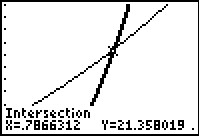
\includegraphics[width=2in]{./ExpLogsGraphics/ExpEqns03.jpg} &

\hspace{0.75in} 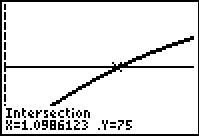
\includegraphics[width=2in]{./ExpLogsGraphics/ExpEqns04.jpg} \\

$y = f(x) = 9 \cdot 3^{x} $ and   & 

 \hspace{0.75in}  $y = f(x) = 75$ and \\
 
 \boldmath $y=g(x) = 7^{2x}$ & 
 \hspace{0.75in} \boldmath $y=g(x) = \frac{100}{1 + 3e^{-2x}}$  \\

\end{tabular}

\end{center}

\item  We start solving $25^{x} = 5^{x} + 6$ by rewriting $25 = 5^2$ so that we have $\left(5^2\right)^{x} = 5^{x} + 6$, or $5^{2x} = 5^{x} + 6$.  Even though we have a common base, having two terms on the right hand side of the equation foils our plan of equating exponents or taking logs.  If we stare at this long enough, we notice that we have three terms with the exponent on one term exactly twice that of another. To our surprise and delight, we have a  `quadratic in disguise'.  Letting $u = 5^{x}$,  we have $u^2 = \left(5^{x}\right)^2 = 5^{2x}$ so the equation $5^{2x} = 5^{x} + 6$ becomes $u^2 = u + 6$.  Solving this as $u^2 - u - 6=0$ gives $u = -2$ or $u = 3$.  Since $u = 5^{x}$, we have $5^{x} = -2$ or $5^{x} = 3$.  Since $5^{x} = -2$ has no real solution, (Why not?) we focus on $5^{x} = 3$.  Since it isn't convenient to express $3$ as a power of $5$, we take natural logs and get $\ln\left(5^{x}\right) = \ln(3)$ so that $x \ln(5) = \ln(3)$ or $x = \frac{\ln(3)}{\ln(5)}$.  On the calculator, we see the graphs of $f(x) = 25^{x}$ and $g(x) = 5^{x} + 6$ intersect at $x=\frac{\ln(3)}{\ln(5)} \approx 0.6826$.

\item  At first, it's unclear how to proceed with $\frac{e^{x} - e^{-x}}{2} = 5$, besides clearing the denominator to obtain $e^{x} - e^{-x} = 10$.  Of course, if we rewrite $e^{-x} = \frac{1}{e^{x}}$, we see we have another denominator lurking in the problem:  $e^{x} - \frac{1}{e^{x}} = 10$. Clearing this denominator gives us $e^{2x} - 1 = 10e^{x}$, and once again, we have an equation with three terms where the exponent on one term is exactly twice that of another - a `quadratic in disguise.'  If we let $u = e^{x}$, then $u^2 = e^{2x}$ so the equation $e^{2x} - 1 = 10e^{x}$ can be viewed as $u^2-1 = 10u$.  Solving $u^2 - 10u - 1 = 0$, we obtain by the quadratic formula $u = 5 \pm \sqrt{26}$.  From this, we have $e^{x} = 5 \pm \sqrt{26}$.  Since $5 - \sqrt{26} < 0$, we get no real solution to $e^{x} = 5 - \sqrt{26}$, but for $e^{x} = 5 + \sqrt{26}$, we take natural logs to obtain $x = \ln\left(5 + \sqrt{26}\right)$.  If we graph $f(x) = \frac{e^{x} - e^{-x}}{2}$ and $g(x) = 5$, we see that the graphs intersect at $x = \ln\left(5 + \sqrt{26}\right) \approx 2.312$

\begin{center}

\begin{tabular}{cc}

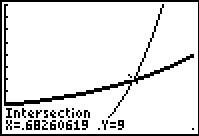
\includegraphics[width=2in]{./ExpLogsGraphics/ExpEqns05.jpg} &

\hspace{0.75in} 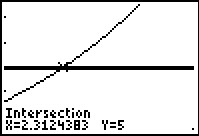
\includegraphics[width=2in]{./ExpLogsGraphics/ExpEqns06.jpg} \\

$y = f(x) = 25^{x}  $ and   & 

 \hspace{0.75in}  $y = f(x) = \frac{e^{x} - e^{-x}}{2}$ and \\
 
 \boldmath $y=g(x) = 5^{x} + 6$ & 
 \hspace{0.75in} \boldmath $y=g(x) = 5$  \\

\end{tabular}

\end{center}

\end{enumerate}

\qed

\end{ex}

The authors would be remiss not to mention that Example \ref{expeqnsex1} still holds great educational value.  Much can be learned about logarithms and exponentials by verifying the solutions obtained in Example \ref{expeqnsex1} analytically. For example, to verify our solution to  $2000 = 1000 \cdot 3^{-0.1 t}$, we substitute $t = -\frac{10\ln(2)}{\ln(3)}$ and obtain 
\[ \begin{array}{rclr}

2000 & \stackrel{?}{=} & 1000 \cdot 3^{-0.1 \left(-\frac{10\ln(2)}{\ln(3)}\right)} & \\
2000 & \stackrel{?}{=} & 1000 \cdot 3^{\frac{\ln(2)}{\ln(3)}} & \\
2000 & \stackrel{?}{=} & 1000 \cdot 3^{\log_{3}(2)} & \mbox{Change of Base}\\
2000 & \stackrel{?}{=} & 1000 \cdot 2 & \mbox{Inverse Property}\\
2000 & \stackrel{\checkmark}{=} & 2000 & \\

\end{array}\]

The other solutions can be verified by using a combination of log and inverse properties.  Some fall out quite quickly, while others are more involved.  We leave them to the reader.

\smallskip

Since exponential functions are continuous on their domains, the Intermediate Value Theorem \ref{IVT} applies.  As with the algebraic functions in Section \ref{AlgebraicFunctions}, this allows us to solve inequalities using sign diagrams as demonstrated below.

\begin{ex}  Solve the following inequalities.  Check your answer graphically using a calculator.
\label{expineq}

\begin{multicols}{3}

\begin{enumerate}

\item  $2^{x^2-3x} - 16 \geq 0$

\item  $\dfrac{e^{x}}{e^{x}-4} \leq 3$

\item  $x e^{2x} < 4x$

\end{enumerate}

\end{multicols}

{\bf Solution.}

\begin{enumerate}

\item  Since we already have $0$ on one side of the inequality, we set $r(x) = 2^{x^2-3x} - 16$.  The domain of $r$ is all real numbers, so in order to construct our sign diagram, we seed to find the zeros of $r$.  Setting $r(x) = 0$ gives $2^{x^2-3x} - 16 = 0$ or $2^{x^2-3x} = 16$.  Since $16 = 2^{4}$ we have $2^{x^2-3x} = 2^{4}$, so by the one-to-one property of exponential functions, $x^2 -3x = 4$.  Solving $x^2 -3x - 4 = 0$ gives $x=4$ and $x=-1$.  From the sign diagram, we see $r(x) \geq 0$ on $(-\infty, -1] \cup [4, \infty)$, which corresponds to where the graph of  $y=r(x) = 2^{x^2-3x} - 16$, is on or above the $x$-axis.

\begin{center}

\begin{tabular}{m{2in}c}

\begin{mfpic}[10]{-5}{5}{-1}{2}
\arrow \reverse \arrow \polyline{(-5,0),(5,0)}
\xmarks{-2,2}
\tlabel[cc](-3.5,1){$(+)$}
\tlabel[cc](-2,-1){$-1$}
\tlabel[cc](-2,1){$0$}
\tlabel[cc](0,1){$(-)$}
\tlabel[cc](2,-1){$4$}
\tlabel[cc](2,1){$0$}
\tlabel[cc](3.5,1){$(+)$}
\end{mfpic}

& 

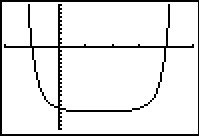
\includegraphics[width=2in]{./ExpLogsGraphics/ExpEqns07.jpg} \\

& $y=r(x) = 2^{x^2-3x} - 16$ \\

\end{tabular}

\end{center}

\item The first step we need to take to solve  $\frac{e^{x}}{e^{x}-4} \leq 3$ is to get $0$ on one side of the inequality. To that end, we subtract $3$ from both sides and get a common denominator


\setlength{\extrarowheight}{12pt}
\[ \begin{array}{rclr}

\dfrac{e^{x}}{e^{x}-4} & \leq & 3 & \\

\dfrac{e^{x}}{e^{x}-4} - 3 & \leq & 0 & \\

\dfrac{e^{x}}{e^{x}-4} - \dfrac{3 \left(e^{x}-4\right)}{e^{x}-4} & \leq & 0 & \mbox{Common denomintors.} \\

\dfrac{12 - 2e^{x}}{e^{x}-4} & \leq & 0 & \\

\end{array}\]
\setlength{\extrarowheight}{2pt}

We set $r(x) = \frac{12 - 2e^{x}}{e^{x}-4}$ and we note that $r$ is undefined when its denominator $e^{x}-4=0$, or when $e^{x} = 4$.  Solving this gives $x = \ln(4)$, so the domain of $r$ is $(-\infty, \ln(4)) \cup (\ln(4), \infty)$. To find the zeros of $r$, we solve $r(x) = 0$ and obtain $12 - 2e^{x} = 0$.  Solving for $e^{x}$, we find $e^{x} = 6$, or $x = \ln(6)$.  When we build our sign diagram, finding test values may be a little tricky since we need to check values around $\ln(4)$ and $\ln(6)$.  Recall that the function $\ln(x)$ is increasing\footnote{This is because the base of $\ln(x)$ is $e > 1$.  If the base $b$ were in the interval $0 < b < 1$, then $\log_{b}(x)$ would decreasing.} which means $\ln(3) < \ln(4) < \ln(5) < \ln(6) < \ln(7)$.  While the prospect of determining the sign of $r\left(\ln(3)\right)$ may be very unsettling, remember that $e^{\ln(3)} = 3$, so \[r\left(\ln(3)\right) = \frac{12 - 2e^{\ln(3)}}{e^{\ln(3)}-4} = \frac{12-2(3)}{3-4} = -6\]  We determine the signs of $r\left(\ln(5)\right)$ and $r\left(\ln(7)\right)$ similarly.\footnote{We could, of course, use the calculator, but what fun would that be?} From the sign diagram, we find our answer to be $(-\infty,\ln(4)) \cup [\ln(6), \infty)$.  Using the calculator, we see the graph of $f(x) = \frac{e^{x}}{e^{x}-4}$ is below the graph of $g(x) = 3$ on $(-\infty,\ln(4)) \cup (\ln(6), \infty)$, and they intersect at $x = \ln(6) \approx 1.792$.


\begin{center}

\begin{tabular}{m{2in}c}

\begin{mfpic}[10]{-5}{5}{-1}{2}
\arrow \reverse \arrow \polyline{(-5,0),(5,0)}
\xmarks{-2,2}
\tlabel[cc](-3.5,1){$(-)$}
\tlabel[cc](-2,-1){$\ln(4)$}
\tlabel[cc](-2,1){\textinterrobang}
\tlabel[cc](0,1){$(+)$}
\tlabel[cc](2,-1){$\ln(6)$}
\tlabel[cc](2,1){$0$}
\tlabel[cc](3.5,1){$(-)$}
\end{mfpic}

& 

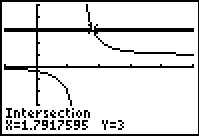
\includegraphics[width=2in]{./ExpLogsGraphics/ExpEqns08.jpg} \\

& $y = f(x) = \frac{e^{x}}{e^{x} - 4}$ \\
& \boldmath $y = g(x) = 3$

\end{tabular}

\end{center}


\item  As before, we start solving $x e^{2x} < 4x$ by getting $0$ on one side of the inequality, $x e^{2x} - 4x < 0$.   We set $r(x) = xe^{2x} - 4x$ and since there are no denominators, even-indexed radicals, or logs, the domain of $r$ is all real numbers.  Setting $r(x) = 0$  produces $x e^{2x} - 4x  = 0$. We factor to get $x \left(e^{2x} - 4\right)  = 0$ which gives $x=0$ or $e^{2x} - 4 = 0$.  To solve the latter, we isolate the exponential and take logs to get $2x = \ln(4)$, or $x = \frac{\ln(4)}{2} = \ln(2)$.  (Can you explain the last equality using properties of logs?)  As in the previous example, we need to be careful about choosing test values.  Since $\ln(1) = 0$, we choose $\ln\left(\frac{1}{2}\right)$, $\ln\left(\frac{3}{2}\right)$ and $\ln(3)$.  Evaluating,\footnote{A calculator can be used at this point. As usual, we proceed without apologies, with the analytical method.} we get 

\[\begin{array}{rclr}

r\left(\ln\left(\frac{1}{2}\right)\right) & = & \ln\left(\frac{1}{2}\right) e^{2\ln\left(\frac{1}{2}\right)} - 4\ln\left(\frac{1}{2}\right) & \\

&= & \ln\left(\frac{1}{2}\right)e^{\ln\left(\frac{1}{2}\right)^2}- 4\ln\left(\frac{1}{2}\right) & \text{Power Rule} \\

& = & \ln\left(\frac{1}{2}\right)e^{\ln\left(\frac{1}{4}\right)}- 4\ln\left(\frac{1}{2}\right) & \\

& = & \frac{1}{4}  \ln\left(\frac{1}{2}\right) - 4  \ln\left(\frac{1}{2}\right) =  -\frac{15}{4} \ln\left(\frac{1}{2}\right) & \end{array}\] 

Since $\frac{1}{2} < 1$, $ \ln\left(\frac{1}{2}\right) < 0$ and we get $r(\ln\left(\frac{1}{2}\right))$ is $(+)$, so $r(x) < 0$ on $(0 ,\ln(2))$.  The calculator confirms that the graph of $f(x) = x e^{2x} $ is below the graph of $g(x) = 4x$ on these intervals.\footnote{Note: $\ln(2) \approx 0.693$.}
\enlargethispage{.5in}

\begin{center}

\begin{tabular}{m{2in}c}

\begin{mfpic}[10]{-5}{5}{-1}{2}
\arrow \reverse \arrow \polyline{(-5,0),(5,0)}
\xmarks{-2,2}
\tlabel[cc](-3.5,1){$(+)$}
\tlabel[cc](-2,-1){$0$}
\tlabel[cc](-2,1){0}
\tlabel[cc](0,1){$(-)$}
\tlabel[cc](2,-1){$\ln(2)$}
\tlabel[cc](2,1){$0$}
\tlabel[cc](3.5,1){$(+)$}
\end{mfpic}

& 

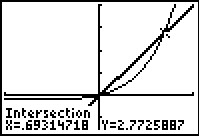
\includegraphics[width=2in]{./ExpLogsGraphics/ExpEqns09.jpg} \\

& $y=f(x) =x e^{2x}$  and \boldmath $y = g(x) = 4x$ \\

\end{tabular}

\end{center}

\end{enumerate}

\qed

\end{ex}

\begin{ex}  Recall from Example \ref{exptempex} that the temperature of coffee $T$ (in degrees Fahrenheit) $t$ minutes after it is served can be modeled by $T(t) = 70 + 90 e^{-0.1 t}$.  When will the coffee be warmer than $100^{\circ}\mbox{F}$?
\smallskip

{\bf Solution.}  We need to find when $T(t) > 100$, or in other words, we need to solve the inequality  $70 + 90 e^{-0.1 t} > 100$.  Getting $0$ on one side of the inequality, we have  $90 e^{-0.1 t} - 30 > 0$, and we set $r(t) = 90 e^{-0.1 t} - 30$.  The domain of $r$ is artificially restricted due to the context of the problem to   $[0, \infty)$, so we proceed to find the zeros of $r$.  Solving $90 e^{-0.1 t} - 30=0$ results in $e^{-0.1t} = \frac{1}{3}$ so that $t = -10\ln\left(\frac{1}{3}\right)$ which, after a quick application of the Power Rule leaves us with $t = 10 \ln(3)$.  If we wish to avoid using the calculator to choose test values, we note that since $1 < 3$, $0 = \ln(1) < \ln(3)$ so that $10\ln(3) > 0$.  So we choose $t = 0$ as a test value in $[0, 10 \ln(3))$.  Since $3 < 4$, $10 \ln(3) < 10 \ln(4)$, so the latter is our choice of a test value for the interval $(10 \ln(3), \infty)$.  Our sign diagram is below, and next to it is our graph of $t=T(t)$ from Example  \ref{exptempex} with the horizontal line $y = 100$.   

\begin{center}

\begin{tabular}{m{0.5in}m{2.5in}m{2.5in}}

&

\begin{mfpic}[10]{0}{8}{-2}{2}
\arrow \polyline{(0,0), (8,0)}
\xmarks{0,4}
\tlabel[cc](0,-1){$0$}
\tlabel[cc](0,1){$(+)$}
\tlabel[cc](4,-1){\scriptsize $10 \ln(3)$}
\tlabel[cc](4,1){$0$}
\tlabel[cc](6,1){$(-)$}
\end{mfpic}

& 

\begin{mfpic}[10]{-1}{11}{-1}{10}
\point[2pt]{(0,8)}
\dashed \polyline{(-1,3.5),(11,3.5)}
\axes
\tlabel[cc](9,2.5){\tiny H.A. $y=70$}
\tlabel[cc](9,5.5){\tiny $y=100$}
\tlabel[cc](11,-0.5){\tiny $t$}
\tlabel[cc](0.5,10){\tiny $y$}
\tcaption{\scriptsize $y = T(t)$}
\ymarks{1,2,3,4,5,6,7,8,9}
\xmarks{1,2,3,4,5,6,7,8,9,10}
\tlpointsep{4pt}
\axislabels {x}{{\tiny $2$} 1, {\tiny $4$} 2, {\tiny $6$} 3, {\tiny $8$} 4,{\tiny $10$} 5, {\tiny $12$} 6, {\tiny $14$} 7, {\tiny $16$} 8, {\tiny $18$} 9, {\tiny $20$} 10}
\axislabels {y}{{\tiny $20$} 1, {\tiny $40$} 2, {\tiny $60$} 3,{\tiny $80$} 4, {\tiny $120$} 6,{\tiny $140$} 7, {\tiny $160$} 8, {\tiny $180$} 9}
\arrow \function{0, 10, 0.1}{(90*exp(0-0.2*x)+70)/20}
\penwd{1.1pt}
\arrow \reverse \arrow \polyline{(-1,5),(11,5)}
\end{mfpic} \\

\end{tabular}

\end{center}

In order to interpret what this means in the context of the real world, we need a reasonable approximation of the number $10 \ln(3) \approx 10.986$.  This means it takes approximately $11$ minutes for the coffee to cool to $100^{\circ}\mbox{F}$.  Until then, the coffee is warmer than that.\footnote{Critics may point out that since we needed to use the calculator to interpret our answer anyway, why not use it earlier to simplify the computations? It is a fair question which we answer unfairly:  it's our book.} \qed
\end{ex}

We close this section by finding the inverse of a function which is a composition of a rational function with an exponential function.

\begin{ex}  \label{expfracinverse} The function $f(x) = \dfrac{5e^{x}}{e^{x}+1}$ is one-to-one.  Find a formula for $f^{-1}(x)$ and check your answer graphically using your calculator.

{\bf Solution.}  We start by writing $y=f(x)$, and interchange the roles of $x$ and $y$.  To solve for $y$, we first clear denominators and then isolate the exponential function.

\[ \begin{array}{rclr}
y & = & \dfrac{5e^{x}}{e^{x}+1} & \\ [12pt]
x & = & \dfrac{5e^{y}}{e^{y}+1} & \mbox{Switch $x$ and $y$} \\ [12pt]
x \left(e^{y}+1\right) & = & 5e^{y} & \\ [4pt]
x e^{y}+x & = & 5e^{y} & \\ [4pt]
x & = & 5e^{y} - x e^{y} & \\ [4pt]
x & = & e^{y}(5 - x) & \\ [4pt]
e^{y}& = & \dfrac{x}{5-x} & \\[12pt]
\ln\left(e^{y}\right) & = & \ln\left(\dfrac{x}{5-x}\right) & \\[12pt]
y & = & \ln\left(\dfrac{x}{5-x}\right) & \\
\end{array}\]

We claim $f^{-1}(x) = \ln\left(\frac{x}{5-x}\right)$.  To verify this analytically, we would need to verify the compositions $\left(f^{-1} \circ f\right)(x) = x$ for all $x$ in the domain of $f$ and that $\left(f \circ f^{-1}\right)(x) = x$ for all $x$ in the domain of $f^{-1}$.  We leave this to the reader.  To verify our solution graphically, we graph $y = f(x) = \frac{5e^{x}}{e^{x}+1}$ and $y = g(x) = \ln\left(\frac{x}{5-x}\right)$ on the same set of axes and observe the symmetry about the line $y=x$.  Note the domain of $f$ is the range of $g$ and vice-versa.

\begin{center}
\begin{tabular}{c}

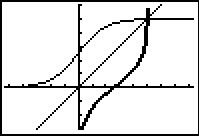
\includegraphics[width=2in]{./ExpLogsGraphics/ExpEqns10.jpg} \\

$y = f(x) = \frac{5e^{x}}{e^{x}+1}$ and \boldmath $y = g(x) = \ln\left(\frac{x}{5-x}\right)$ \\

\end{tabular}
\end{center}

\qed

\end{ex}

\newpage

\subsection{Exercises}


In Exercises \ref{expeqnfirst} - \ref{expeqnlast}, solve the equation analytically.

\begin{multicols}{3}
\begin{enumerate}

\item $2^{4x} = 8$  \label{expeqnfirst} 
\item $3^{(x - 1)} = 27$  
\item $5^{2x-1} = 125$ 

\setcounter{HW}{\value{enumi}}
\end{enumerate}
\end{multicols}

\begin{multicols}{3}
\begin{enumerate}
\setcounter{enumi}{\value{HW}}

\item $4^{2x} = \frac{1}{2}$
\item $8^{x} = \frac{1}{128}$ 
\item $2^{(x^{3} - x)} = 1$ 

\setcounter{HW}{\value{enumi}}
\end{enumerate}
\end{multicols}

\begin{multicols}{3}
\begin{enumerate}
\setcounter{enumi}{\value{HW}}

\item $3^{7x} = 81^{4-2x}$ 
\item $9 \cdot 3^{7x} = \left(\frac{1}{9}\right)^{2x}$ 
\item $3^{2x} = 5$ 

\setcounter{HW}{\value{enumi}}
\end{enumerate}
\end{multicols}

\begin{multicols}{3}
\begin{enumerate}
\setcounter{enumi}{\value{HW}}

\item $5^{-x} = 2$ 
\item $5^{x} = -2$  
\item $3^{(x - 1)} = 29$  

\setcounter{HW}{\value{enumi}}
\end{enumerate}
\end{multicols}

\begin{multicols}{3}
\begin{enumerate}
\setcounter{enumi}{\value{HW}}

\item $(1.005)^{12x} = 3$
\item $e^{-5730k} = \frac{1}{2}$ 
\item $2000e^{0.1t} = 4000$  

\setcounter{HW}{\value{enumi}}
\end{enumerate}
\end{multicols}

\begin{multicols}{3}
\begin{enumerate}
\setcounter{enumi}{\value{HW}}


\item $500\left(1-e^{2x}\right) = 250$
\item $70 + 90e^{-0.1t} = 75$ 
\item $30-6e^{-0.1x}=20$ 


\setcounter{HW}{\value{enumi}}
\end{enumerate}
\end{multicols}

\begin{multicols}{3}
\begin{enumerate}
\setcounter{enumi}{\value{HW}}

\item $\dfrac{100e^{x}}{e^{x}+2}=50$ 
\item $\dfrac{5000}{1+2e^{-3t}}=2500$ 
\item $\dfrac{150}{1 + 29e^{-0.8t}} = 75$ 


\setcounter{HW}{\value{enumi}}
\end{enumerate}
\end{multicols}

\begin{multicols}{3}
\begin{enumerate}
\setcounter{enumi}{\value{HW}}

\item $25\left(\frac{4}{5}\right)^{x} = 10$  

\item $e^{2x} = 2e^{x}$ 
\item  $7e^{2x} = 28e^{-6x}$ 

\setcounter{HW}{\value{enumi}}
\end{enumerate}
\end{multicols}

\begin{multicols}{3}
\begin{enumerate}
\setcounter{enumi}{\value{HW}}

\item $3^{(x - 1)} = 2^{x}$ 
\item $3^{(x - 1)} = \left(\frac{1}{2}\right)^{(x + 5)}$ 
\item  $7^{3+7x} = 3^{4-2x}$  

\setcounter{HW}{\value{enumi}}
\end{enumerate}
\end{multicols}

\begin{multicols}{3}
\begin{enumerate}
\setcounter{enumi}{\value{HW}}

\item $e^{2x} - 3e^{x}-10=0$ %Ans $x=\ln(5)$
\item $e^{2x} = e^{x}+6$ %Ans $x=\ln(2)$
\item $4^{x} + 2^{x} = 12$ %Ans $x=\frac{\ln(3)}{\ln(2)}$


\setcounter{HW}{\value{enumi}}
\end{enumerate}
\end{multicols}

\begin{multicols}{3}
\begin{enumerate}
\setcounter{enumi}{\value{HW}}

\item $e^{x}-3e^{-x}=2$ %Ans $x=\ln(3)$
\item $e^{x}+15e^{-x}=8$ %Ans $x=\ln(2)$, $\ln(5)$
\item $3^{x}+25\cdot3^{-x}=10$ %Ans $x=\frac{\ln(5)}{\ln(3)}$
\label{expeqnlast} 

\setcounter{HW}{\value{enumi}}
\end{enumerate}
\end{multicols}



In Exercises \ref{expineqfirst} - \ref{expineqlast}, solve the inequality analytically.

\begin{multicols}{2} 
\begin{enumerate}
\setcounter{enumi}{\value{HW}}

\item $e^{x} > 53$ \label{expineqfirst} 
\item $1000\left(1.005\right)^{12t} \geq 3000$ 

\setcounter{HW}{\value{enumi}}
\end{enumerate}
\end{multicols}

\begin{multicols}{2} 
\begin{enumerate}
\setcounter{enumi}{\value{HW}}

\item $2^{(x^{3} - x)} < 1$
\item $25\left(\frac{4}{5}\right)^{x} \geq 10$

\setcounter{HW}{\value{enumi}}
\end{enumerate}
\end{multicols}

\begin{multicols}{2} 
\begin{enumerate}
\setcounter{enumi}{\value{HW}}

\item $\dfrac{150}{1 + 29e^{-0.8t}} \leq 130$

\item $\vphantom{\dfrac{150}{1 + 29e^{-0.8t}}} 70 + 90e^{-0.1t} \leq 75$ \label{expineqlast}

\setcounter{HW}{\value{enumi}}
\end{enumerate}
\end{multicols}


In Exercises \ref{calcexpineqfirst} - \ref{calcexpineqlast},  use your calculator to help you solve the equation or  inequality.

\begin{multicols}{3} 
\begin{enumerate}
\setcounter{enumi}{\value{HW}}

\item $2^{x} = x^2$ \label{calcexpineqfirst} 
\item $e^{x} = \ln(x) + 5$   
\item $e^{\sqrt{x}} = x + 1$ 



\setcounter{HW}{\value{enumi}}
\end{enumerate}
\end{multicols}

\begin{multicols}{3} 
\begin{enumerate}
\setcounter{enumi}{\value{HW}}


\item $e^{-x} - xe^{-x} \geq 0$
\item $3^{(x - 1)} < 2^{x}$ 
\item $e^{x} < x^{3} - x$ \label{calcexpineqlast} 


\setcounter{HW}{\value{enumi}}
\end{enumerate}
\end{multicols}


\begin{enumerate}
\setcounter{enumi}{\value{HW}}

\item \label{onetoonelogexercise} Since $f(x) = \ln(x)$ is a strictly increasing function, if $0 < a < b$ then $\ln(a) < \ln(b)$.  Use this fact to solve the inequality $e^{(3x - 1)} > 6$ without a sign diagram. Use this technique to solve the inequalities in Exercises \ref{expineqfirst} - \ref{expineqlast}. (NOTE:  Isolate the exponential function first!)

\item \label{hyperbolicsine} Compute the inverse of $f(x) = \dfrac{e^{x} - e^{-x}}{2}$.  State the domain and range of both $f$ and $f^{-1}$. 

\item In Example \ref{expfracinverse}, we found that the inverse of $f(x) = \dfrac{5e^{x}}{e^{x}+1}$ was $f^{-1}(x) = \ln\left(\dfrac{x}{5-x}\right)$ but we left a few loose ends for you to tie up.  

\begin{enumerate}

\item Show that $\left(f^{-1} \circ f\right)(x) = x$ for all $x$ in the domain of $f$ and that $\left(f \circ f^{-1}\right)(x) = x$ for all $x$ in the domain of $f^{-1}$.

\item Find the range of $f$ by finding the domain of $f^{-1}$.

\item Let $g(x) = \dfrac{5x}{x+1}$ and $h(x) = e^{x}$.  Show that $f = g \circ h$ and that $(g \circ h)^{-1} = h^{-1} \circ g^{-1}$. 
(We know this is true in general by Exercise \ref{fcircginverse} in Section \ref{InverseFunctions}, but it's nice to see a specific example of the property.)

\end{enumerate}

\item With the help of your classmates, solve the inequality $e^{x} > x^{n}$ for a variety of natural numbers $n$.  What might you conjecture about the ``speed'' at which $f(x) = e^{x}$ grows versus any polynomial?

\end{enumerate}

\newpage

\subsection{Answers}


\begin{multicols}{3}
\begin{enumerate}

\item $x = \frac{3}{4}$
\item $x = 4$
\item $x=2$

\setcounter{HW}{\value{enumi}}
\end{enumerate}
\end{multicols}

\begin{multicols}{3}
\begin{enumerate}
\setcounter{enumi}{\value{HW}}

\item $x = -\frac{1}{4}$
\item $x = -\frac{7}{3}$
\item $x = -1, \, 0, \, 1$

\setcounter{HW}{\value{enumi}}
\end{enumerate}
\end{multicols}

\begin{multicols}{3}
\begin{enumerate}
\setcounter{enumi}{\value{HW}}

\item $x = \frac{16}{15}$
\item $x=-\frac{2}{11}$
\item $x = \frac{\ln(5)}{2\ln(3)}$

\setcounter{HW}{\value{enumi}}
\end{enumerate}
\end{multicols}

\begin{multicols}{3}
\begin{enumerate}
\setcounter{enumi}{\value{HW}}

\item $x = -\frac{\ln(2)}{\ln(5)}$
\item No solution.
\item $x = \frac{\ln(29) + \ln(3)}{\ln(3)}$

\setcounter{HW}{\value{enumi}}
\end{enumerate}
\end{multicols}

\begin{multicols}{3}
\begin{enumerate}
\setcounter{enumi}{\value{HW}}

\item $x = \frac{\ln(3)}{12\ln(1.005)}$
\item $k = \frac{\ln\left(\frac{1}{2}\right)}{-5730} = \frac{1}{5730} \ln(2)$
\item $t=\frac{\ln(2)}{0.1} = 10\ln(2)$

\setcounter{HW}{\value{enumi}}
\end{enumerate}
\end{multicols}

\begin{multicols}{2}
\begin{enumerate}
\setcounter{enumi}{\value{HW}}


\item $x=\frac{1}{2}\ln\left(\frac{1}{2}\right) = -\frac{1}{2}\ln(2)$
\item $t = \frac{\ln\left(\frac{1}{18}\right)}{-0.1} =10 \ln(18)$



\setcounter{HW}{\value{enumi}}
\end{enumerate}
\end{multicols}

\begin{multicols}{2}
\begin{enumerate}
\setcounter{enumi}{\value{HW}}


\item $x=-10\ln\left(\frac{5}{3}\right) = 10\ln\left(\frac{3}{5}\right)$
\item$x=\ln(2)$

\setcounter{HW}{\value{enumi}}
\end{enumerate}
\end{multicols}

\begin{multicols}{2}
\begin{enumerate}
\setcounter{enumi}{\value{HW}}

\item $t=\frac{1}{3}\ln(2)$
\item $t = \frac{\ln\left(\frac{1}{29}\right)}{-0.8} = \frac{5}{4}\ln(29)$

\setcounter{HW}{\value{enumi}}
\end{enumerate}
\end{multicols}

\begin{multicols}{2}
\begin{enumerate}
\setcounter{enumi}{\value{HW}}

\item $x = \frac{\ln\left(\frac{2}{5}\right)}{\ln\left(\frac{4}{5}\right)} = \frac{\ln(2)-\ln(5)}{\ln(4) - \ln(5)}$

\item $x =  \ln(2)$


\setcounter{HW}{\value{enumi}}
\end{enumerate}
\end{multicols}

\begin{multicols}{2}
\begin{enumerate}
\setcounter{enumi}{\value{HW}}


\item  $x = -\frac{1}{8} \ln\left(\frac{1}{4} \right) = \frac{1}{4}\ln(2)$

\item $x = \frac{\ln(3)}{\ln(3) - \ln(2)}$

\setcounter{HW}{\value{enumi}}
\end{enumerate}
\end{multicols}

\begin{multicols}{2}
\begin{enumerate}
\setcounter{enumi}{\value{HW}}


\item $x = \frac{\ln(3) + 5\ln\left(\frac{1}{2}\right)}{\ln(3) - \ln\left(\frac{1}{2}\right)} = \frac{\ln(3)-5\ln(2)}{\ln(3)+\ln(2)}$
\item  $x = \frac{4 \ln(3) - 3 \ln(7)}{7 \ln(7) + 2 \ln(3)}$

\setcounter{HW}{\value{enumi}}
\end{enumerate}
\end{multicols}

\begin{multicols}{3}
\begin{enumerate}
\setcounter{enumi}{\value{HW}}

\item $x=\ln(5)$
\item $x=\ln(3)$
\item $x=\frac{\ln(3)}{\ln(2)}$


\setcounter{HW}{\value{enumi}}
\end{enumerate}
\end{multicols}

\begin{multicols}{3}
\begin{enumerate}
\setcounter{enumi}{\value{HW}}

\item $x=\ln(3)$
\item $x=\ln(3)$, $\ln(5)$
\item $x=\frac{\ln(5)}{\ln(3)}$


\setcounter{HW}{\value{enumi}}
\end{enumerate}
\end{multicols}

\begin{multicols}{2} 
\begin{enumerate}
\setcounter{enumi}{\value{HW}}

\item $(\ln(53), \infty)$
\item $\left[\frac{\ln(3)}{12\ln(1.005)}, \infty\right)$

\setcounter{HW}{\value{enumi}}
\end{enumerate}
\end{multicols}

\begin{multicols}{2} 
\begin{enumerate}
\setcounter{enumi}{\value{HW}}

\item $(-\infty, -1) \cup (0, 1)$
\item $\left(-\infty, \frac{\ln\left(\frac{2}{5}\right)}{\ln\left(\frac{4}{5}\right)} \right] = \left(-\infty, \frac{\ln(2)-\ln(5)}{\ln(4)-\ln(5)} \right]$

\setcounter{HW}{\value{enumi}}
\end{enumerate}
\end{multicols}

\begin{multicols}{2} 
\begin{enumerate}
\setcounter{enumi}{\value{HW}}

\item $\left(-\infty, \frac{\ln\left(\frac{2}{377}\right)}{-0.8} \right] = \left(-\infty, \frac{5}{4}\ln\left(\frac{377}{2}\right) \right]$
\item $\left[\frac{\ln\left(\frac{1}{18}\right)}{-0.1}, \infty\right) = [10\ln(18), \infty)$

\setcounter{HW}{\value{enumi}}
\end{enumerate}
\end{multicols}

\begin{multicols}{2} 
\begin{enumerate}
\setcounter{enumi}{\value{HW}}

\item $x \approx -0.76666, \, x = 2, \, x = 4$
\item $x \approx 0.01866, \, x \approx 1.7115$


\setcounter{HW}{\value{enumi}}
\end{enumerate}
\end{multicols}

\begin{multicols}{2} 
\begin{enumerate}
\setcounter{enumi}{\value{HW}}

\item $x = 0$
\item $(-\infty, 1]$

\setcounter{HW}{\value{enumi}}
\end{enumerate}
\end{multicols}

\begin{multicols}{2} 
\begin{enumerate}
\setcounter{enumi}{\value{HW}}

\item $\approx (-\infty, 2.7095)$
\item $\approx (2.3217, 4.3717)$


\setcounter{HW}{\value{enumi}}
\end{enumerate}
\end{multicols}


\begin{enumerate}
\setcounter{enumi}{\value{HW}}

\item $x > \frac{1}{3}(\ln(6) + 1)$

\item  $f^{-1} = \ln\left(x + \sqrt{x^{2} + 1}\right)$. Both $f$ and $f^{-1}$ have domain $(-\infty, \infty)$ and range $(-\infty, \infty)$.


\end{enumerate}

\closegraphsfile

\newpage

\section{Logarithmic Equations and Inequalities}

\mfpicnumber{1}

\opengraphsfile{LogEquations}

\setcounter{footnote}{0}

\label{LogEquations}

In Section \ref{ExpEquations} we solved equations and inequalities involving exponential functions using one of two basic strategies.  We now turn our attention to equations and inequalities involving logarithmic functions, and not surprisingly, there are two basic strategies to choose from.  For example, suppose we wish  to solve $\log_{2}(x) = \log_{2}(5)$.  Theorem \ref{explogsonetoone} tells us that the \textit{only} solution to this equation is $x=5$.  Now suppose we wish to solve $\log_{2}(x) = 3$.  If we want to use Theorem \ref{explogsonetoone}, we need to rewrite $3$ as a logarithm base $2$.   We can use Theorem \ref{invpropslogs} to do just that: $3 = \log_{2}\left(2^{3}\right) = \log_{2}(8)$.  Our equation then becomes  $\log_{2}(x) =  \log_{2}(8)$ so that $x = 8$.  However, we could have arrived at the same answer,  in fewer steps, by using Theorem \ref{invpropslogs} to rewrite the equation $\log_{2}(x) = 3$ as $2^{3} = x$, or $x=8$.  We summarize the two common ways to solve log equations below.

\smallskip

\colorbox{ResultColor}{\bbm

\centerline{\textbf{Steps for Solving an Equation involving Logarithmic Functions}} \index{logarithm ! solving equations with} 

\begin{enumerate}

\item  Isolate the logarithmic function.

\item  \begin{enumerate}

\item  If convenient, express both sides as logs with the same base and equate the arguments of the log functions.

\item  Otherwise, rewrite the log equation as an exponential equation.


\end{enumerate}

\end{enumerate}

\ebm}

\smallskip

\begin{ex}  \label{LogEqnsEx1} Solve the following equations.  Check your solutions graphically using a calculator.

\begin{multicols}{2}
\begin{enumerate}

\item  $\log_{117}(1-3x) = \log_{117}\left(x^2-3\right)$

\item  $2 - \ln(x-3) = 1$

\setcounter{HW}{\value{enumi}}
\end{enumerate}
\end{multicols}

\begin{multicols}{2}
\begin{enumerate}
\setcounter{enumi}{\value{HW}}

\item  $\log_{6}(x+4) + \log_{6}(3-x) = 1$

\item  $\log_{7}(1-2x) = 1 - \log_{7}(3-x)$
\setcounter{HW}{\value{enumi}}
\end{enumerate}
\end{multicols}

\begin{multicols}{2}
\begin{enumerate}
\setcounter{enumi}{\value{HW}}

\item  $\log_{2}(x+3) = \log_{2}(6-x)+3$

\item  $1 + 2 \log_{4}(x+1) = 2 \log_{2}(x)$

\end{enumerate}
\end{multicols}

{\bf Solution.}

\begin{enumerate}

\item  Since we have the same base on both sides of the equation $\log_{117}(1-3x) = \log_{117}\left(x^2-3\right)$, we equate what's inside the logs to get $1-3x = x^2-3$.  Solving $x^2+3x-4 = 0$ gives $x=-4$ and $x=1$. To check these answers using the calculator, we make use of the change of base formula and graph $f(x) = \frac{\ln(1-3x)}{\ln(117)}$ and $g(x) = \frac{\ln\left(x^2-3\right)}{\ln(117)}$ and we see they intersect only at $x=-4$.  To see what happened to the solution $x=1$, we substitute it into our original equation to obtain  $\log_{117}(-2) =  \log_{117}(-2)$.  While these expressions look identical, neither is a real number,\footnote{They do, however, represent the same \textbf{family} of complex numbers.  We stop ourselves at this point and refer the reader to a good course in Complex Variables.} which means $x=1$ is not in the domain of the original equation, and is not a solution.    

\item  Our first objective in solving $2 - \ln(x-3) = 1$ is to isolate the logarithm.  We get $\ln(x-3)=1$, which, as an exponential equation, is $e^{1} = x-3$.  We get our solution $x=e+3$. On the calculator, we see the graph of $f(x) = 2 - \ln(x-3)$ intersects  the graph of $g(x) = 1$ at $x = e+3 \approx 5.718$.

\begin{center}

\begin{tabular}{cc}

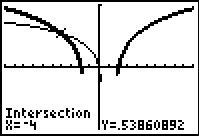
\includegraphics[width=2in]{./ExpLogsGraphics/LogEqns01.jpg} &

\hspace{0.75in} 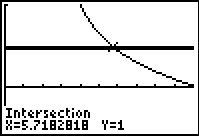
\includegraphics[width=2in]{./ExpLogsGraphics/LogEqns02.jpg} \\

$y = f(x) =\log_{117}(1-3x)$ and   & 

 \hspace{0.75in}  $y = f(x) =  2 - \ln(x-3)$ and \\
 
 \boldmath $y=g(x) =\log_{117}\left(x^2-3\right)$ & 
 \hspace{0.75in} \boldmath $y=g(x) = 1$  \\

\end{tabular}

\end{center}

\item We can start solving $\log_{6}(x+4) + \log_{6}(3-x) = 1$ by using the Product Rule for logarithms to rewrite the equation as  $\log_{6}\left[(x+4)(3-x)\right] = 1$.  Rewriting this as an exponential equation, we get $6^{1} = (x+4)(3-x)$.  This reduces to $x^2+x-6 = 0$, which gives $x=-3$ and $x=2$.   Graphing $y=f(x) =  \frac{\ln(x+4)}{\ln(6)} + \frac{\ln(3-x)}{\ln(6)}$ and $y=g(x) = 1$, we see they intersect twice, at $x=-3$ and $x=2$.

\begin{center}

\begin{tabular}{cc}

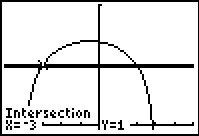
\includegraphics[width=2in]{./ExpLogsGraphics/LogEqns03.jpg} &

\hspace{0.75in} 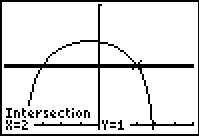
\includegraphics[width=2in]{./ExpLogsGraphics/LogEqns04.jpg} \\

\end{tabular}

$y = f(x) =\log_{6}(x+4) + \log_{6}(3-x)$ and  \boldmath  $y=g(x) = 1$

\end{center}

\item  Taking a cue from the previous problem, we begin solving $\log_{7}(1-2x) = 1 - \log_{7}(3-x)$ by first collecting the logarithms on the same side, $\log_{7}(1-2x) +  \log_{7}(3-x) = 1$, and then using the Product Rule to get $\log_{7}[(1-2x)(3-x)] = 1$.  Rewriting this as an exponential equation gives $7^{1} = (1-2x)(3-x)$ which gives the quadratic equation $2x^2-7x-4=0$.  Solving, we find  $x = -\frac{1}{2}$ and $x=4$.  Graphing, we find $y = f(x) = \frac{\ln(1-2x)}{\ln(7)}$ and $y=g(x) = 1 - \frac{\ln(3-x)}{\ln(7)}$ intersect only at $x=-\frac{1}{2}$.  Checking $x=4$ in the original equation produces $\log_{7}(-7) = 1 - \log_{7}(-1)$, which is a clear domain violation.

\item Starting with  $\log_{2}(x+3) = \log_{2}(6-x)+3$, we gather the logarithms to one side and get $\log_{2}(x+3) - \log_{2}(6-x) = 3$.  We then use the Quotient Rule and convert to an exponential equation \[\log_{2}\left(\frac{x+3}{6-x}\right) = 3 \iff 2^{3} = \frac{x+3}{6-x} \] This reduces to the linear equation $8(6-x) = x+3$, which gives us $x = 5$.  When we graph $f(x) = \frac{\ln(x+3)}{\ln(2)}$ and $g(x) =  \frac{\ln(6-x)}{\ln(2)} + 3$, we find they intersect at $x=5$.

\begin{center}

\begin{tabular}{cc}

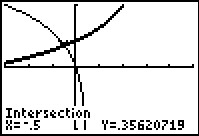
\includegraphics[width=2in]{./ExpLogsGraphics/LogEqns05.jpg} &

\hspace{0.75in} 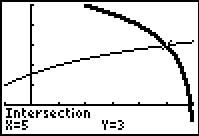
\includegraphics[width=2in]{./ExpLogsGraphics/LogEqns06.jpg} \\

$y = f(x) =\log_{7}(1-2x)$ and   & 

 \hspace{0.75in}  $y = f(x) =  \log_{2}(x+3)$ and \\
 
 \boldmath $y=g(x)=1 - \log_{7}(3-x)$ & 
 \hspace{0.75in} \boldmath $y=g(x) = \log_{2}(6-x)+3$  \\

\end{tabular}

\end{center}

\item Starting with $1 + 2 \log_{4}(x+1) = 2 \log_{2}(x)$, we gather the logs to one side to get the equation $1 = 2 \log_{2}(x) - 2 \log_{4}(x+1)$.  Before we can combine the logarithms, however, we need a common base.  Since $4$ is a power of $2$, we use change of base to convert  \[\log_{4}(x+1) = \frac{\log_{2}(x+1)}{\log_{2}(4)} = \frac{1}{2} \log_{2}(x+1)\] Hence, our original equation becomes  

\[ \begin{array}{rclr}

1 & = & 2 \log_{2}(x) - 2 \left(\frac{1}{2} \log_{2}(x+1)\right) & \\ [2pt]
1 &= & 2\log_{2}(x) - \log_{2}(x+1) & \\ [2pt]
1 & = & \log_{2}\left(x^2\right) - \log_{2}(x+1) & \text{Power Rule} \\ [6pt]
1 & = & \log_{2}\left( \dfrac{x^{2}}{x+1}\right) & \text{Quotient Rule} \\ \end{array}\]

Rewriting this in exponential form, we get $ \frac{x^{2}}{x+1} = 2$ or $x^2 -2x-2 = 0$.  Using the quadratic formula, we get $x = 1 \pm \sqrt{3}$.  Graphing $f(x) = 1 + \frac{2\ln(x+1)}{\ln(4)}$ and $g(x) = \frac{2 \ln(x)}{\ln(2)}$, we see the graphs intersect only at $x = 1 + \sqrt{3} \approx 2.732$.  The solution $x = 1 - \sqrt{3} < 0$, which means if substituted into the original equation, the term $2 \log_{2}\left(1 - \sqrt{3}\right)$ is undefined.

\begin{center}
\begin{tabular}{c}

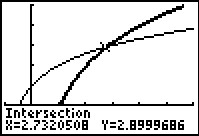
\includegraphics[width=2in]{./ExpLogsGraphics/LogEqns07.jpg} \\

$y = f(x) = 1 + 2 \log_{4}(x+1)$ and \boldmath $y = g(x) = 2 \log_{2}(x)$ \\

\end{tabular}
\end{center}
\end{enumerate}

\qed
\end{ex}

If nothing else,  Example \ref{LogEqnsEx1} demonstrates the importance of checking for extraneous solutions\footnote{Recall that an extraneous solution is an answer obtained analytically which does not satisfy the original equation.} when solving equations involving logarithms.  Even though we checked our answers graphically, extraneous solutions are easy to spot - any supposed solution which causes a negative number inside a logarithm needs to be discarded.  As with the equations in Example \ref{expeqnsex1}, much can be learned from checking all of the answers in Example \ref{LogEqnsEx1} analytically.  We leave this to the reader and turn our attention to inequalities involving logarithmic functions.  Since logarithmic functions are continuous on their domains, we can use sign diagrams.  

\begin{ex}  Solve the following inequalities.  Check your answer graphically using a calculator.
\label{logineq}

\begin{multicols}{3}

\begin{enumerate}

\item  $\dfrac{1}{\ln(x)+1} \leq 1$

\item  $\left(\log_{2}(x)\right)^2 < 2 \log_{2}(x) + 3$

\item  $x \log(x+1) \geq x$


\end{enumerate}

\end{multicols}


{\bf Solution.}  

\begin{enumerate}

\item  We start solving $\frac{1}{\ln(x)+1} \leq 1$ by getting $0$ on one side of the inequality: $\frac{1}{\ln(x)+1}  - 1 \leq 0$.  Getting a common denominator yields $\frac{1}{\ln(x)+1}  - \frac{\ln(x)+1}{\ln(x)+1} \leq 0$ which reduces to $\frac{-\ln(x)}{\ln(x)+1} \leq 0$, or $ \frac{\ln(x)}{\ln(x)+1} \geq 0$.  We define $r(x) = \frac{\ln(x)}{\ln(x)+1}$ and set about finding the domain and the zeros of $r$.  Due to the appearance of the term $\ln(x)$, we require  $x > 0$.  In order to keep the denominator away from zero, we solve $\ln(x)+1 = 0$ so $\ln(x) = -1$, so $x = e^{-1} = \frac{1}{e}$.  Hence, the domain of $r$ is $\left(0, \frac{1}{e}\right) \cup \left(\frac{1}{e}, \infty\right)$.  To find the zeros of $r$, we set $r(x) = \frac{\ln(x)}{\ln(x)+1} = 0$ so that $\ln(x) = 0$, and we find $x = e^{0} = 1$.  In order to determine test values for $r$ without resorting to the calculator, we need to find numbers between $0$, $\frac{1}{e}$, and $1$ which have a base of $e$.  Since $e \approx 2.718 > 1$, $0 < \frac{1}{e^2} < \frac{1}{e} < \frac{1}{\sqrt{e}} < 1 < e$.  To determine the sign of $r\left( \frac{1}{e^2} \right)$, we use the fact that $\ln\left(\frac{1}{e^2}\right) = \ln\left(e^{-2}\right) = -2$, and find $r\left( \frac{1}{e^2} \right) = \frac{-2}{-2+1} = 2$, which is $(+)$.  The rest of the test values are determined similarly.   From our sign diagram, we find the solution to be $\left(0, \frac{1}{e}\right) \cup [1, \infty)$. Graphing $f(x) =  \frac{1}{\ln(x)+1}$ and $g(x) = 1$, we see the graph of $f$ is below the graph of $g$ on the solution intervals, and that the graphs intersect at $x=1$.

\begin{center}

\begin{tabular}{m{2in}c}

\begin{mfpic}[10]{-6}{6}{-2}{2}
\arrow \polyline{(-6,0),(6,0)}
\xmarks{-6,-2,2}
\tiny
\tlpointsep{6pt}
\normalsize
\tlabel[cc](-6,-1){$0$}
\tlabel[cc](-4,1){$(+)$}
\tlabel[cc](-2,-1){$\frac{1}{e}$}
\tlabel[cc](-2,1){\textinterrobang}
\tlabel[cc](0,1){$(-)$}
\tlabel[cc](2,-1){$1$}
\tlabel[cc](2,1){$0$}
\tlabel[cc](4,1){$(+)$}
\end{mfpic} 

& 

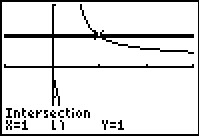
\includegraphics[width=2in]{./ExpLogsGraphics/LogEqns08.jpg} \\

& $y=f(x) = \frac{1}{\ln(x)+1}$ and \boldmath $y = g(x) = 1$ \\

\end{tabular}

\end{center}

\item  Moving all of the nonzero terms of  $\left(\log_{2}(x)\right)^2 < 2 \log_{2}(x) + 3$ to one side of the inequality, we have $\left(\log_{2}(x)\right)^2 - 2 \log_{2}(x) - 3 < 0$. Defining $r(x) = \left(\log_{2}(x)\right)^2 - 2 \log_{2}(x) - 3$, we get the domain of $r$ is $(0, \infty)$, due to the presence of the logarithm.  To find the zeros of $r$, we set $r(x) =\left(\log_{2}(x)\right)^2 - 2 \log_{2}(x) - 3= 0$ which results in a `quadratic in disguise.'  We set $u = \log_{2}(x)$ so our equation becomes $u^2-2u-3 = 0$ which gives us $u=-1$ and $u=3$.  Since $u = \log_{2}(x)$, we get $\log_{2}(x) = -1$, which gives us $x = 2^{-1} = \frac{1}{2}$, and $\log_{2}(x) = 3$, which yields $x = 2^{3} = 8$.  We use test values which are powers of $2$: $0 < \frac{1}{4} < \frac{1}{2} < 1 < 8 < 16$, and from our sign diagram, we see $r(x)< 0$ on $\left(\frac{1}{2}, 8 \right)$. Geometrically, we see the graph of $f(x)= \left(\frac{\ln(x)}{\ln(2)}\right)^2$ is below  the graph of $y = g(x) = \frac{2 \ln(x)}{\ln(2)} + 3$ on the solution interval.

\begin{center}

\begin{tabular}{m{2in}c}

\begin{mfpic}[10]{-6}{6}{-2}{2}
\arrow \polyline{(-6,0),(6,0)}
\xmarks{-6,-2,2}
\tiny
\tlpointsep{6pt}
\normalsize
\tlabel[cc](-6,-1){$0$}
\tlabel[cc](-4,1){$(+)$}
\tlabel[cc](-2,-1){$\frac{1}{2}$}
\tlabel[cc](-2,1){$0$}
\tlabel[cc](0,1){$(-)$}
\tlabel[cc](2,-1){$8$}
\tlabel[cc](2,1){$0$}
\tlabel[cc](4,1){$(+)$}
\end{mfpic} 

& 

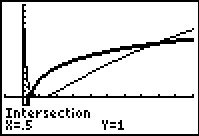
\includegraphics[width=2in]{./ExpLogsGraphics/LogEqns09.jpg} \\

& $y=f(x) = \left(\log_{2}(x)\right)^2$ and \boldmath $y = g(x) = 2 \log_{2}(x) + 3$ \\

\end{tabular}

\end{center}

\item  We begin to solve $x \log(x+1) \geq x$ by subtracting $x$ from both sides to get $x \log(x+1)  - x \geq 0$.  We define $r(x) = x \log(x+1)  - x $ and due to the presence of the logarithm, we require $x+1 > 0$, or $x > -1$.  To find the zeros of $r$, we set $r(x) = x \log(x+1)  - x = 0$.  Factoring, we get $x \left(\log(x+1) - 1\right) = 0$, which gives $x=0$ or $\log(x+1) - 1=0$.  The latter gives $\log(x+1) = 1$, or $x+1 = 10^{1}$, which admits $x = 9$.  We select test values $x$ so that $x+1$ is a power of $10$, and we obtain $-1 < -0.9 < 0 < \sqrt{10} -1 < 9 < 99$.  Our sign diagram gives the solution to be $(-1,0] \cup [9, \infty)$. The calculator indicates the graph of $y= f(x) = x \log(x+1)$ is above $y=g(x) = x$ on the solution intervals, and the graphs intersect at $x=0$ and $x=9$.


\begin{center}

\begin{tabular}{m{2in}c}

\begin{mfpic}[10]{-6}{6}{-2}{2}
\arrow \polyline{(-6,0),(6,0)}
\xmarks{-6,-2,2}
\tiny
\tlpointsep{4pt}
\normalsize
\tlabel[cc](-6,-1){$-1$}
\tlabel[cc](-4,1){$(+)$}
\tlabel[cc](-2,-1){$0$}
\tlabel[cc](-2,1){$0$}
\tlabel[cc](0,1){$(-)$}
\tlabel[cc](2,-1){$9$}
\tlabel[cc](2,1){$0$}
\tlabel[cc](4,1){$(+)$}
\end{mfpic} 

& 

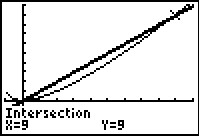
\includegraphics[width=2in]{./ExpLogsGraphics/LogEqns10.jpg} \\

& $y=f(x) = x \log(x+1)$ and \boldmath $y = g(x) = x$ \\

\end{tabular}

\end{center} 

\end{enumerate}

\qed

\end{ex}

\smallskip

Our next example revisits the concept of pH first seen in Exercise \ref{pHexercise} in Section \ref{IntroExpLogs}.  


\begin{ex}

In order to successfully breed Ippizuti fish the pH of a freshwater tank must be at least 7.8 but can be no more than 8.5.  Determine the corresponding range of hydrogen ion concentration, and check your answer using a calculator.

\smallskip

{\bf Solution.}  Recall from Exercise \ref{pHexercise} in Section \ref{IntroExpLogs} that $\mbox{pH} = -\log[\mbox{H}^{+}]$ where $[\mbox{H}^{+}]$ is the hydrogen ion concentration in moles per liter.  We require $7.8 \leq -\log[\mbox{H}^{+}] \leq 8.5$ or $-7.8 \geq \log[\mbox{H}^{+}] \geq -8.5$.  To solve this compound inequality we solve $-7.8 \geq \log[\mbox{H}^{+}]$ and $ \log[\mbox{H}^{+}] \geq -8.5$ and take the intersection of the solution sets.\footnote{Refer to page \pageref{intersectionunion} for a discussion of what this means.}  The former inequality yields $0 < [\mbox{H}^{+}] \leq 10^{-7.8}$ and the latter yields $[\mbox{H}^{+}] \geq 10^{-8.5}$.  Taking the intersection gives us our final answer $10^{-8.5} \leq [\mbox{H}^{+}] \leq 10^{-7.8}$.  (Your Chemistry professor may want the answer written as $3.16 \times 10^{-9} \leq [\mbox{H}^{+}] \leq 1.58 \times 10^{-8}$.)  After carefully adjusting the viewing window on the graphing calculator we see that the graph of $f(x) = -\log(x)$ lies between the lines $y = 7.8$ and $y = 8.5$ on the interval $[3.16 \times 10^{-9}, 1.58 \times 10^{-8}]$.

\smallskip

\begin{center}

\begin{tabular}{cc}

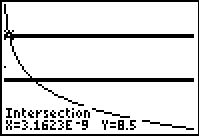
\includegraphics[width=2in]{./ExpLogsGraphics/LogEqns13.jpg}  \hspace{0.75in} & 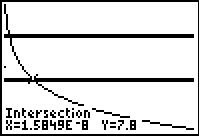
\includegraphics[width=2in]{./ExpLogsGraphics/LogEqns14.jpg}  \\

\end{tabular}

\end{center}

\centerline{The graphs of $y = f(x) = -\log(x)$, \boldmath $y = 7.8$ and \boldmath $y = 8.5$}

\qed

\end{ex}

\smallskip

We close this section by finding an inverse of a one-to-one function which involves logarithms.

\begin{ex}  \label{logfracinverse} The function $f(x) = \dfrac{\log(x)}{1-\log(x)}$ is one-to-one.  Find a formula for $f^{-1}(x)$ and check your answer graphically using your calculator.

{\bf Solution.}  We first write $y=f(x)$ then interchange the $x$ and $y$ and solve for $y$.

\[ \begin{array}{rclr}
y & = & f(x) & \\ 
y  & = & \dfrac{\log(x)}{1-\log(x)} & \\[8pt]
x  & = & \dfrac{\log(y)}{1-\log(y)} & \mbox{Interchange $x$ and $y$.}\\[8pt]
x\left(1-\log(y)\right) & = & \log(y) & \\ 
x - x\log(y)  & = & \log(y) & \\ 
x & = & x \log(y) + \log(y) & \\ 
x & = & (x+1) \log(y) & \\ 
\dfrac{x}{x+1}  & = & \log(y) & \\ 
y & = & 10^{\frac{x}{x+1}} & \mbox{Rewrite as an exponential equation.}\\

\end{array}\]

\pagebreak

We have $f^{-1}(x) = 10^{\frac{x}{x+1}}$.  Graphing $f$ and $f^{-1}$ on the same viewing window yields

\begin{center}
\begin{tabular}{c}

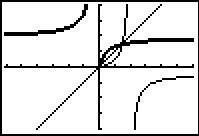
\includegraphics[width=2in]{./ExpLogsGraphics/LogEqns15.jpg} \\

$y = f(x) = \dfrac{\log(x)}{1-\log(x)}$ and \boldmath $y = g(x) = 10^{\frac{x}{x+1}}$ \\

\end{tabular}
\end{center}

\qed

\end{ex}

\newpage
\subsection{Exercises}

In Exercises \ref{solvelogeqexfirst} - \ref{solvelogeqexlast}, solve the equation analytically.

\begin{multicols}{2}
\begin{enumerate}

\item $\log(3x-1) = \log(4-x)$  \label{solvelogeqexfirst}

\item $\log_{2}\left(x^{3}\right) = \log_{2}(x)$

\setcounter{HW}{\value{enumi}}
\end{enumerate}
\end{multicols}

\begin{multicols}{2}
\begin{enumerate}
\setcounter{enumi}{\value{HW}}

\item $\ln\left(8-x^2\right)=\ln(2-x)$

\item $\log_{5}\left(18-x^2\right) = \log_{5}(6-x)$

\setcounter{HW}{\value{enumi}}
\end{enumerate}
\end{multicols}

\begin{multicols}{2}
\begin{enumerate}
\setcounter{enumi}{\value{HW}}

\item $\log_{3}(7-2x) = 2$
\item $\log_{\frac{1}{2}} (2x-1) = -3$

\setcounter{HW}{\value{enumi}}
\end{enumerate}
\end{multicols}

\begin{multicols}{2}
\begin{enumerate}
\setcounter{enumi}{\value{HW}}

\item $\ln\left(x^2-99\right) = 0$
\item $\log(x^2-3x) = 1$

\setcounter{HW}{\value{enumi}}
\end{enumerate}
\end{multicols}

\begin{multicols}{2}
\begin{enumerate}
\setcounter{enumi}{\value{HW}}

\item $\log_{125} \left(\dfrac{3x-2}{2x+3}\right)=\dfrac{1}{3}$

\item $\log\left(\dfrac{x}{10^{-3}}\right) = 4.7$ \vphantom{$\log_{125} \left(\dfrac{3x-2}{2x+3}\right)$} \label{sixfourRichterequ}


\setcounter{HW}{\value{enumi}}
\end{enumerate}
\end{multicols}


\begin{multicols}{2}
\begin{enumerate}
\setcounter{enumi}{\value{HW}}

\item $-\log(x) = 5.4$ \vphantom{$10\log\left(\dfrac{x}{10^{-12}}\right)$} \label{sixfourpHequ}
\item $10\log\left(\dfrac{x}{10^{-12}}\right) = 150$ \label{sixfourdecibelequ}

\setcounter{HW}{\value{enumi}}
\end{enumerate}
\end{multicols}

\begin{multicols}{2}
\begin{enumerate}
\setcounter{enumi}{\value{HW}}

\item $6-3\log_{5}(2x)=0$
\item $3\ln(x)-2=1-\ln(x)$

\setcounter{HW}{\value{enumi}}
\end{enumerate}
\end{multicols}

\begin{multicols}{2}
\begin{enumerate}
\setcounter{enumi}{\value{HW}}

\item $\log_{3}(x - 4) + \log_{3}(x + 4) = 2$

\item $\log_{5}(2x + 1) + \log_{5}(x + 2) = 1$

\setcounter{HW}{\value{enumi}}
\end{enumerate}
\end{multicols}

\begin{multicols}{2}
\begin{enumerate}
\setcounter{enumi}{\value{HW}}

\item $\log_{169}(3x + 7) - \log_{169}(5x - 9) = \dfrac{1}{2}$

\item $\ln(x+1) - \ln(x) = 3$ \vphantom{$\log_{169}(3x + 7)$}

\setcounter{HW}{\value{enumi}}
\end{enumerate}
\end{multicols}

\begin{multicols}{2}
\begin{enumerate}
\setcounter{enumi}{\value{HW}}

\item $2\log_{7}(x) = \log_{7}(2) + \log_{7}(x+12)$

\item $\log(x) - \log(2) = \log(x+8)  - \log(x+2)$

\setcounter{HW}{\value{enumi}}
\end{enumerate}
\end{multicols}

\begin{multicols}{2}
\begin{enumerate}
\setcounter{enumi}{\value{HW}}

\item $\log_{3}(x) = \log_{\frac{1}{3}}(x) + 8$

\item $\ln(\ln(x)) = 3$

\setcounter{HW}{\value{enumi}}
\end{enumerate}
\end{multicols}

\begin{multicols}{2}
\begin{enumerate}
\setcounter{enumi}{\value{HW}}

\item $\left(\log(x)\right)^2=2\log(x)+15$

\item $\ln(x^{2}) = (\ln(x))^{2}$ \label{solvelogeqexlast}

\setcounter{HW}{\value{enumi}}
\end{enumerate}
\end{multicols}


In Exercises \ref{solvelogineqexfirst} - \ref{solvelogineqexlast}, solve the inequality analytically.

\begin{multicols}{2}
\begin{enumerate}
\setcounter{enumi}{\value{HW}}

\item $\dfrac{1 - \ln(x)}{x^{2}} < 0$ \label{solvelogineqexfirst}
\item $x\ln(x) - x > 0$ \phantom{$\dfrac{1 - \ln(x)}{x^{2}} < 0$}


\setcounter{HW}{\value{enumi}}
\end{enumerate}
\end{multicols}

\begin{multicols}{2}
\begin{enumerate}
\setcounter{enumi}{\value{HW}}

\item $10\log\left(\dfrac{x}{10^{-12}}\right) \geq 90$ \label{sixfourdecibelineq} 
\item $5.6 \leq \log\left(\dfrac{x}{10^{-3}}\right) \leq 7.1$ \label{sixfourRichterineq}


\setcounter{HW}{\value{enumi}}
\end{enumerate}
\end{multicols}

\begin{multicols}{2}
\begin{enumerate}
\setcounter{enumi}{\value{HW}}


\item $2.3 < -\log(x) < 5.4$ \label{sixfourpHineq} 

\item $\ln(x^{2}) \leq (\ln(x))^{2}$ \label{solvelogineqexlast} 

\setcounter{HW}{\value{enumi}}
\end{enumerate}
\end{multicols}

In Exercises \ref{logeqcalcexfirst} - \ref{logeqcalcexlast}, use your calculator to help you solve the equation or  inequality.

\begin{multicols}{2}
\begin{enumerate}
\setcounter{enumi}{\value{HW}}

\item $\ln(x) = e^{-x}$ \label{logeqcalcexfirst} 
\item $\ln(x) = \sqrt[4]{x}$ 

\setcounter{HW}{\value{enumi}}
\end{enumerate}
\end{multicols}

\begin{multicols}{2}
\begin{enumerate}
\setcounter{enumi}{\value{HW}}

\item $\ln(x^{2} + 1) \geq 5$
\item $\ln(-2x^{3} - x^{2} + 13x - 6) < 0$ \label{logeqcalcexlast} 

\setcounter{HW}{\value{enumi}}
\end{enumerate}
\end{multicols}

\begin{enumerate}
\setcounter{enumi}{\value{HW}}

\item \label{onetooneexpexercise} Since $f(x) = e^{x}$ is a strictly increasing function, if $a < b$ then $e^{a} < e^{b}$.  Use this fact to solve the inequality $\ln(2x + 1) < 3$ without a sign diagram. Use this technique to solve the inequalities in Exercises \ref{sixfourdecibelineq} - \ref{sixfourpHineq}. (Compare this to Exercise  \ref{onetoonelogexercise} in Section \ref{ExpEquations}.)

\item Solve $\ln(3 - y) - \ln(y) = 2x + \ln(5)$ for $y$.

\item In Example \ref{logfracinverse} we found the inverse of $f(x) = \dfrac{\log(x)}{1-\log(x)}$ to be $f^{-1}(x) = 10^{\frac{x}{x+1}}$.

\begin{enumerate}

\item Show that $\left(f^{-1} \circ f\right)(x) = x$ for all $x$ in the domain of $f$ and that $\left(f \circ f^{-1}\right)(x) = x$ for all $x$ in the domain of $f^{-1}$.

\item Find the range of $f$ by finding the domain of $f^{-1}$.

\item Let $g(x) = \dfrac{x}{1 - x}$ and $h(x) = \log(x)$.  Show that $f = g \circ h$ and $(g \circ h)^{-1} = h^{-1} \circ g^{-1}$.\\
(We know this is true in general by Exercise \ref{fcircginverse} in Section \ref{InverseFunctions}, but it's nice to see a specific example of the property.)

\end{enumerate}

\item \label{inversehyptangent} Let $f(x) = \dfrac{1}{2}\ln\left(\dfrac{1 + x}{1 - x}\right)$.  Compute $f^{-1}(x)$ and find its domain and range.

\item Explain the equation in Exercise \ref{sixfourRichterequ} and the inequality in Exercise \ref{sixfourRichterineq} above in terms of the Richter scale for earthquake magnitude.  (See Exercise \ref{Richterexercise} in Section \ref{IntroExpLogs}.)

\item Explain the equation in Exercise \ref{sixfourdecibelequ} and the inequality in Exercise \ref{sixfourdecibelineq} above in terms of sound intensity level as measured in decibels.  (See Exercise \ref{decibelexercise} in Section \ref{IntroExpLogs}.)

\item Explain the equation in Exercise \ref{sixfourpHequ} and the inequality in Exercise \ref{sixfourpHineq} above in terms of the pH of a solution.  (See Exercise \ref{pHexercise} in Section \ref{IntroExpLogs}.)

\item With the help of your classmates, solve the inequality $\sqrt[n]{x} > \ln(x)$ for a variety of natural numbers $n$.  What might you conjecture about the ``speed'' at which $f(x) = \ln(x)$ grows versus any principal $n^{\textrm{th}}$ root function?

\end{enumerate}

\newpage

\subsection{Answers}
\begin{multicols}{3}
\begin{enumerate}

\item $x = \frac{5}{4}$
\item $x = 1$
\item $x=-2$

\setcounter{HW}{\value{enumi}}
\end{enumerate}
\end{multicols}

\begin{multicols}{3}
\begin{enumerate}
\setcounter{enumi}{\value{HW}}

\item $x=-3,\, 4$
\item $x=-1$
\item $x=\frac{9}{2}$

\setcounter{HW}{\value{enumi}}
\end{enumerate}
\end{multicols}

\begin{multicols}{3}
\begin{enumerate}
\setcounter{enumi}{\value{HW}}

\item $x=\pm 10$
\item $x=-2,\, 5$
\item $x = -\frac{17}{7}$

\setcounter{HW}{\value{enumi}}
\end{enumerate}
\end{multicols}

\begin{multicols}{3}
\begin{enumerate}
\setcounter{enumi}{\value{HW}}

\item $x = 10^{1.7}$
\item $x = 10^{-5.4}$
\item $x = 10^{3}$

\setcounter{HW}{\value{enumi}}
\end{enumerate}
\end{multicols}

\begin{multicols}{3}
\begin{enumerate}
\setcounter{enumi}{\value{HW}}

\item $x=\frac{25}{2}$
\item $x=e^{3/4}$
\item $x = 5$

\setcounter{HW}{\value{enumi}}
\end{enumerate}
\end{multicols}

\begin{multicols}{3}
\begin{enumerate}
\setcounter{enumi}{\value{HW}}

\item $x = \frac{1}{2}$
\item $x = 2$
\item $x = \frac{1}{e^3-1}$

\setcounter{HW}{\value{enumi}}
\end{enumerate}
\end{multicols}

\begin{multicols}{3}
\begin{enumerate}
\setcounter{enumi}{\value{HW}}

\item $x=6$
\item $x=4$
\item $x = 81$

\setcounter{HW}{\value{enumi}}
\end{enumerate}
\end{multicols}

\begin{multicols}{3}
\begin{enumerate}
\setcounter{enumi}{\value{HW}}

\item $x = e^{e^3}$
\item $x=10^{-3}, \, 10^{5}$
\item $x = 1, \, x = e^{2}$

\setcounter{HW}{\value{enumi}}
\end{enumerate}
\end{multicols}

\begin{multicols}{3}
\begin{enumerate}
\setcounter{enumi}{\value{HW}}

\item $(e, \infty)$
\item $(e, \infty)$
\item $\left[10^{-3}, \infty \right)$

\setcounter{HW}{\value{enumi}}
\end{enumerate}
\end{multicols}

\begin{multicols}{3}
\begin{enumerate}
\setcounter{enumi}{\value{HW}}

\item $\left[10^{2.6}, 10^{4.1}\right]$

\item $\left(10^{-5.4}, 10^{-2.3}\right)$
\item $(0, 1] \cup [e^{2}, \infty)$

\setcounter{HW}{\value{enumi}}
\end{enumerate}
\end{multicols}

\begin{multicols}{2}
\begin{enumerate}
\setcounter{enumi}{\value{HW}}

\item $x \approx 1.3098$
\item $x \approx 4.177, \, x \approx 5503.665$

\setcounter{HW}{\value{enumi}}
\end{enumerate}
\end{multicols}

\begin{multicols}{2}
\begin{enumerate}
\setcounter{enumi}{\value{HW}}

\item $\approx (-\infty, -12.1414) \cup (12.1414, \infty)$
\item $\approx (-3.0281, -3) \cup (0.5, 0.5991) \cup (1.9299, 2)$

\setcounter{HW}{\value{enumi}}
\end{enumerate}
\end{multicols}

\begin{multicols}{2}
\begin{enumerate}
\setcounter{enumi}{\value{HW}}

\item $-\dfrac{1}{2} < x < \dfrac{e^{3} - 1}{2}$

\item $y = \dfrac{3}{5e^{2x} + 1}$ \vphantom{$\dfrac{e^{3} - 1}{2}$}

\setcounter{HW}{\value{enumi}}
\end{enumerate}
\end{multicols}

\begin{enumerate}
\setcounter{enumi}{\value{HW}}
\addtocounter{enumi}{1}

\item $f^{-1}(x) = \dfrac{e^{2x} - 1}{e^{2x} + 1} = \dfrac{e^{x} - e^{-x}}{e^{x} + e^{-x}}$. (To see why we rewrite this in this form, see  Exercise \ref{andtheresthyperbolic} in Section \ref{Parametric}.)  The domain of $f^{-1}$ is $(-\infty, \infty)$ and its range is the same as the domain of $f$, namely $(-1, 1)$.

\end{enumerate}

\closegraphsfile

\newpage

\section{Applications of Exponential and Logarithmic Functions}

\opengraphsfile{ExpLogApplications}

\setcounter{footnote}{0}

\label{ExpLogApplications}

As we mentioned in Section \ref{IntroExpLogs}, exponential and logarithmic functions are used to model a wide variety of behaviors in the real world.  In the examples that follow, note that while the applications are drawn from many different disciplines, the mathematics remains essentially the same.  Due to the applied nature of the problems we will examine in this section, the calculator is often used to express our answers as decimal approximations.

\subsection{Applications of Exponential Functions}
\label{expapp}

Perhaps the most well-known application of exponential functions comes from the financial world.  Suppose you have $ \$ 100$ to invest at your local bank and they are offering a whopping $5 \, \%$ annual percentage interest rate.  This means that after one year, the bank will pay \textit{you} $5 \%$ of that $\$100$, or $ \$ 100(0.05) =\$ 5$ in interest, so you now have $\$105$.\footnote{How generous of them!}    This is in accordance with the formula for  \textit{simple interest} which you have undoubtedly run across at some point before.

\smallskip

\colorbox{ResultColor}{\bbm

\begin{eqn} \index{interest ! simple} \index{simple interest} \label{simpleinterest} \textbf{Simple Interest}  The amount of interest $I$ accrued at an annual rate $r$ on an investment\footnote{Called the \index{principal} \textbf{principal}} $P$ after $t$ years is  \[I = Prt\]  The amount $A$ in the account after $t$ years is given by \[A = P + I = P + Prt = P(1+rt)\]

\end{eqn}

\ebm}

\smallskip

Suppose, however, that six months into the year, you hear of a better deal at a rival bank.\footnote{Some restrictions may apply.} Naturally, you withdraw your money and try to invest it at the higher rate there.  Since six months is one half of a year, that initial $\$100$ yields $\$100(0.05)\left(\frac{1}{2}\right) = \$ 2.50$ in interest.  You take your $\$102.50$ off to the competitor and find out that those restrictions which \textit{may} apply actually \underline{do} apply to you, and you return to your bank which happily accepts your $\$102.50$ for the remaining six months of the year.  To your surprise and delight, at the end of the year your statement reads $\$105.06$, not $\$105$ as you had expected.\footnote{Actually, the final balance should be $\$105.0625$.}  Where did those extra six cents come from?  For the first six months of the year, interest was earned on the original principal of $\$100$, but for the second six months, interest was earned on $\$102.50$, that is, you earned interest on your interest.  This is the basic concept behind \textbf{compound interest}.  In the previous discussion, we would say that the interest was compounded twice, or semiannually.\footnote{Using this convention, simple interest after one year is the same as compounding the interest only once.}  If more money can be earned by earning interest on interest already earned, a natural question to ask is what happens if the interest is compounded more often, say $4$ times a year, which is every three months, or `quarterly.'  In this case, the money is in the account for three months, or $\frac{1}{4}$ of a year, at a time.  After the first quarter, we have $A = P(1+rt) =  \$100 \left(1 + 0.05 \cdot \frac{1}{4} \right) = \$101.25$.  We now invest the $\$101.25$ for the next three months and find that at the end of the second quarter, we have $A =  \$101.25 \left(1 + 0.05 \cdot \frac{1}{4} \right)\approx \$102.51$.  Continuing in this manner, the balance at the end of the third quarter is $\$103.79$, and, at last, we obtain $\$105.08$.  The extra two cents hardly seems worth it, but we see that we do in fact get more money the more often we compound.  In order to develop a formula for this phenomenon, we need to do some abstract calculations.  Suppose we wish to invest our principal $P$ at an annual rate $r$ and compound the interest $n$ times per year.  This means the money sits in the account $\frac{1}{n}^{\mbox{\tiny th}}$ of a year between compoundings.  Let $A_{k}$ denote the amount in the account after the $k^{\mbox{\tiny th}}$ compounding.  Then $A_{\mbox{\tiny$1$}} = P\left(1 + r\left(\frac{1}{n}\right)\right)$ which simplifies to $A_{\mbox{\tiny$1$}} = P \left(1 + \frac{r}{n}\right)$.  After the second compounding, we use $A_{\mbox{\tiny$1$}}$ as our new principal and get $A_{\mbox{\tiny$2$}} = A_{\mbox{\tiny$1$}} \left(1 + \frac{r}{n}\right) = \left[P \left(1 + \frac{r}{n}\right)\right]\left(1 + \frac{r}{n}\right) = P \left(1 + \frac{r}{n}\right)^2$.  Continuing in this fashion, we get $A_{\mbox{\tiny$3$}} =P \left(1 + \frac{r}{n}\right)^3$, $A_{\mbox{\tiny$4$}} =P \left(1 + \frac{r}{n}\right)^4$, and so on, so that $A_{k} = P \left(1 + \frac{r}{n}\right)^k$.  Since we compound the interest $n$ times per year, after $t$ years, we have $nt$ compoundings. We have just derived the general formula for compound interest below.

\smallskip

\colorbox{ResultColor}{\bbm

\begin{eqn} \index{interest ! compound} \index{compound interest} \label{compoundinterest} \textbf{Compounded Interest:}  If an initial principal $P$ is invested at an annual rate $r$ and the interest is compounded $n$ times per year, the amount $A$ in the account after $t$ years is \[A(t) = P \left(1 + \frac{r}{n}\right)^{nt}\]

\end{eqn}

\ebm}

\smallskip

If we take $P = 100$, $r = 0.05$, and $n = 4$, Equation \ref{compoundinterest} becomes $A(t) = 100\left(1+ \frac{0.05}{4}\right)^{4t}$ which reduces to $A(t) = 100(1.0125)^{4t}$.  To check this new formula against our previous calculations, we find $A\left(\frac{1}{4}\right) = 100(1.0125)^{4 \left(\frac{1}{4}\right)} = 101.25$, $A\left(\frac{1}{2}\right) \approx \$102.51$, $A\left(\frac{3}{4}\right) \approx \$103.79$, and $A(1) \approx \$105.08$.

\begin{ex}  \label{compoundinterestex} Suppose $\$2000$ is invested in an account which offers $7.125 \%$ compounded monthly.

\begin{enumerate}

\item Express the amount $A$ in the account as a function of the term of the investment $t$ in years.

\item  How much is in the account after $5$ years? 

\item  How long will it take for the initial investment to double?

\item  Find and interpret the average rate of change\footnote{See Definition \ref{arc} in Section \ref{LinearFunctions}.} of the amount in the account from the end of the fourth year to the end of the fifth year, and from the end of the thirty-fourth year to the end of the thirty-fifth year.


\end{enumerate}

{\bf Solution.}  

\begin{enumerate}

\item  Substituting $P = 2000$, $r = 0.07125$, and $n = 12$ (since interest is compounded \textit{monthly}) into Equation \ref{compoundinterest} yields $A(t) = 2000\left(1 + \frac{0.07125}{12}\right)^{12t}=2000 (1.0059375)^{12t}$.

\item  Since $t$ represents the length of the investment in years, we substitute $t=5$ into $A(t)$ to find $A(5) = 2000 (1.0059375)^{12(5)} \approx 2852.92$.  After $5$ years, we have approximately $\$2852.92$.

\item  Our initial investment is $\$2000$, so to find the time it takes this to double, we need to find $t$ when $A(t) = 4000$.  We get $2000 (1.0059375)^{12t}=4000$, or $(1.0059375)^{12t}=2$.  Taking natural logs as in Section \ref{ExpEquations}, we get $t = \frac{\ln(2)}{12 \ln(1.0059375)} \approx 9.75$.  Hence, it takes approximately $9$ years $9$ months for the investment to double.

\item  To find the average rate of change of $A$ from the end of the fourth year to the end of the fifth year, we compute $\frac{A(5)-A(4)}{5-4} \approx 195.63$.  Similarly, the average rate of change of $A$ from the end of the thirty-fourth year to the end of the thirty-fifth year is $\frac{A(35)-A(34)}{35-34} \approx 1648.21$.  This means that the value of the investment is increasing at a rate of approximately $\$195.63$ per year between the end of the fourth and fifth years, while that rate jumps to $\$1648.21$ per year between the end of the thirty-fourth and thirty-fifth years.  So, not only is it true that the longer you wait, the more money you have, but also the longer you wait, the faster the money increases.\footnote{In fact, the rate of increase of the amount in the account is exponential as well.  This is the quality that really defines exponential functions and we refer the reader to a course in Calculus.} \qed

\end{enumerate}

\end{ex}

We have observed that the more times you compound the interest per year, the more money you will earn in a year.  Let's push this notion to the limit.\footnote{Once you've had a semester of Calculus, you'll be able to fully appreciate this very lame pun.}  Consider an investment of $\$ 1$ invested at $100 \%$ interest for $1$ year compounded $n$ times a year.  Equation \ref{compoundinterest} tells us that the amount of money in the account after $1$ year is $A = \left(1+\frac{1}{n}\right)^{n}$.  Below is a table of values relating $n$ and $A$.

\[ \begin{array}{|r||r|}  

\hline

 n & A   \\ \hline
1  & 2  \\  \hline
2  & 2.25  \\  \hline
4 & \approx 2.4414  \\  \hline
12 & \approx 2.6130  \\  \hline
360  & \approx  2.7145 \\  \hline
1000  & \approx 2.7169 \\  \hline
10000  & \approx 2.7181  \\  \hline
100000 & \approx 2.7182  \\  \hline
\end{array} \]

As promised, the more compoundings per year, the more money there is in the account, but we also observe that the increase in money is greatly diminishing.  We are witnessing a mathematical `tug of war'.  While we are compounding more times per year, and hence getting interest on our interest more often, the amount of time between compoundings is getting smaller and smaller, so there is less time to build up additional interest. With Calculus, we can show\footnote{Or define, depending on your point of view.} that as $n \rightarrow \infty$, $A = \left(1+\frac{1}{n}\right)^{n} \rightarrow e$, where $e$ is the natural base first presented in Section \ref{IntroExpLogs}.  Taking the number of compoundings per year to infinity results in what is called  \textbf{continuously} compounded interest.  

\smallskip

\colorbox{ResultColor}{\bbm

\begin{thm} \label{whatise} If you invest $\$1$ at $100 \%$ interest compounded continuously, then you will have $\$ e$ at the end of one year. 

\end{thm}

\ebm}

\smallskip

Using this definition of $e$ and a little Calculus, we can take Equation \ref{compoundinterest} and produce a formula for continuously compounded interest.

\smallskip

\colorbox{ResultColor}{\bbm

\begin{eqn} \index{interest ! compounded continuously} \index{continuously compounded interest} \label{continuouscompoundinterest} \textbf{Continuously Compounded Interest:}  If an initial principal $P$ is invested at an annual rate $r$ and the interest is compounded continuously, the amount $A$ in the account after $t$ years is \[A(t) = P e^{rt} \]

\end{eqn}

\ebm}

\smallskip

If we take the scenario of Example \ref{compoundinterestex} and compare monthly compounding to continuous compounding over $35$ years, we find that monthly compounding yields $A(35) = 2000 (1.0059375)^{12(35)}$ which is about  $\$ 24,\!035.28$, whereas continuously compounding gives $A(35) = 2000e^{0.07125 (35)}$ which is about  $\$ 24,\!213.18$ - a difference of less than $1 \%$.

\smallskip

Equations \ref{compoundinterest} and \ref{continuouscompoundinterest} both use exponential functions to describe the growth of an investment.  Curiously enough, the same principles which govern compound interest are also used to model short term growth of populations.  In Biology, \textbf{The Law of Uninhibited Growth} states as its premise that the \textit{instantaneous} \index{instantaneous rate of change} \index{rate of change ! instantaneous} rate at which a population increases at any time is directly proportional to the population at that time.\footnote{The average rate of change of a function over an interval was first introduced in Section \ref{LinearFunctions}.  \textit{Instantaneous} rates of change are the business of Calculus, as is mentioned on Page \pageref{instantaneousrateofchange}.}  In other words, the more organisms there are at a given moment, the faster they reproduce.  Formulating the law as stated results in a differential equation, which requires Calculus to solve.  Its solution is stated below.

\smallskip

\colorbox{ResultColor}{\bbm

\begin{eqn} \index{growth model ! uninhibited} \index{uninhibited growth} \label{lawofuninhibitedgrowth} \textbf{Uninhibited Growth:} If a population increases according to The Law of Uninhibited Growth, the number of organisms $N$ at time $t$ is given by the formula  \[N(t) = N_{\mbox{\tiny$0$}}e^{kt},\] where $N(0) = N_{\mbox{\tiny$0$}}$ (read `$N$ nought') is the initial number of organisms and $k>0$ is the constant of proportionality which satisfies the equation

\[ \left(\mbox{instantaneous rate of change of $N(t)$ at time $t$}\right) = k \, N(t)\]


\end{eqn}

\ebm}

\smallskip 

 It is worth taking some time to compare Equations \ref{continuouscompoundinterest} and \ref{lawofuninhibitedgrowth}.  In  Equation \ref{continuouscompoundinterest}, we use $P$ to denote the initial investment;  in Equation \ref{lawofuninhibitedgrowth}, we use $N_{\mbox{\tiny$0$}}$ to denote the initial population.  In  Equation \ref{continuouscompoundinterest}, $r$ denotes the annual interest rate,  and so it shouldn't be too surprising that the $k$ in Equation \ref{lawofuninhibitedgrowth} corresponds to a growth rate as well.   While Equations \ref{continuouscompoundinterest} and \ref{lawofuninhibitedgrowth} look entirely different, they both represent the same mathematical concept.

\smallskip

\begin{ex}  In order to perform arthrosclerosis research, epithelial cells are harvested from discarded umbilical tissue and grown in the laboratory.  A technician observes that a culture of twelve thousand cells grows to five million cells in one week.  Assuming that the cells follow The Law of Uninhibited Growth, find a formula for the number of cells, $N$, in thousands, after $t$ days.

\smallskip

{\bf Solution.}  We begin with $N(t) = N_{\mbox{\tiny$0$}}e^{kt}$.  Since $N$ is to give the number of cells \textit{in thousands}, we have $N_{\mbox{\tiny$0$}} = 12$, so $N(t) = 12e^{kt}$.  In order to complete the formula, we need to determine the growth rate $k$.  We know that after one week, the number of cells has grown to five million.  Since $t$ measures days and the units of $N$ are in thousands, this translates mathematically to $N(7) = 5000$.  We get the equation $12e^{7k} = 5000$ which gives $k = \frac{1}{7} \ln\left(\frac{1250}{3}\right)$.  Hence,  $N(t) = 12e^{ \frac{t}{7} \ln\left(\frac{1250}{3}\right)}$.  Of course, in practice, we would approximate $k$ to some desired accuracy, say $k \approx 0.8618$, which we can interpret as an $86.18 \%$ daily growth rate for the cells. \qed

\end{ex}

Whereas Equations \ref{continuouscompoundinterest} and \ref{lawofuninhibitedgrowth} model the growth of quantities, we can use equations like them to describe the decline of quantities.  One example we've seen already is Example \ref{cardepreciationex} in Section \ref{IntroExpLogs}.  There, the value of a car declined from its purchase price of $\$25,\!000$ to nothing at all.  Another real world phenomenon which follows suit is radioactive decay.  There are elements which are unstable and emit energy spontaneously.  In doing so, the amount of the element itself diminishes.  The assumption behind this model is that the rate of decay of an element at a particular time is directly proportional to the amount of the element present at that time.  In other words, the more of the element there is, the faster the element decays.  This is precisely the same kind of hypothesis which drives The Law of Uninhibited Growth, and as such, the equation governing radioactive decay is hauntingly similar to Equation \ref{lawofuninhibitedgrowth} with the exception that the rate constant $k$ is negative.

\smallskip

\colorbox{ResultColor}{\bbm

\begin{eqn} \index{radioactive decay} \label{radioactivedecay} \textbf{Radioactive Decay} The amount of a radioactive element $A$ at time $t$ is given by the formula  \[A(t) = A_{\mbox{\tiny$0$}}e^{kt},\] where $A(0) = A_{\mbox{\tiny$0$}}$ is the initial amount of the element and  $k<0$ is the constant of proportionality which satisfies the equation

\[ \left(\mbox{instantaneous rate of change of $A(t)$ at time $t$}\right) = k \, A(t)\]


\end{eqn}

\ebm}

\smallskip 

\begin{ex}  Iodine-131 is a commonly used radioactive isotope used to help detect how well the thyroid is functioning.  Suppose the decay of Iodine-131 follows the model given in Equation \ref{radioactivedecay}, and that the  half-life\footnote{The time it takes for half of the substance to decay.} of Iodine-131 is approximately $8$ days.  If $5$ grams of Iodine-131 is present initially, find a function which gives the amount of Iodine-131, $A$, in grams, $t$ days later.

\smallskip

{\bf Solution.} Since we start with $5$ grams initially, Equation \ref{radioactivedecay} gives $A(t) = 5e^{kt}$.  Since the half-life is $8$ days, it takes $8$ days for half of the Iodine-131 to decay, leaving half of it behind.  Hence, $A(8) = 2.5$ which means $5e^{8k} = 2.5$.  Solving, we get $k = \frac{1}{8} \ln\left(\frac{1}{2}\right) = -\frac{\ln(2)}{8} \approx -0.08664$, which we can interpret as a loss of material at a rate of $8.664 \%$ daily.  Hence, $A(t) = 5 e^{-\frac{t\ln(2)}{8}} \approx 5 e^{-0.08664t}$. \qed

\end{ex}


We now turn our attention to some more mathematically sophisticated models.  One such model is Newton's Law of Cooling, which we first encountered in Example \ref{exptempex} of Section \ref{IntroExpLogs}.   In that example we had a cup of coffee cooling from $160^{\circ}\mbox{F}$ to room temperature $70^{\circ}\mbox{F}$ according to the formula $T(t) = 70 + 90 e^{-0.1 t}$, where $t$ was measured in minutes.  In this situation, we know the physical limit of the temperature of the coffee is room temperature,\footnote{The Second Law of Thermodynamics states that heat can spontaneously flow from a hotter object to a colder one, but not the other way around.  Thus, the coffee could not continue to release heat into the air so as to cool below room temperature.} and the differential equation which gives rise to our formula for $T(t)$ takes this into account.  Whereas the radioactive decay model had a rate of decay at time $t$ directly proportional to the amount of the element which remained at time $t$, Newton's Law of Cooling states that the rate of cooling of the coffee at a given time $t$ is directly proportional to how much of a temperature \underline{gap} exists between the coffee at time $t$ and room temperature, not the temperature of the coffee itself.  In other words, the coffee cools faster when it is first served, and as its temperature nears room temperature, the coffee cools ever more slowly.  Of course, if we take an item from the refrigerator and let it sit out in the kitchen, the object's temperature will rise to room temperature, and since the physics behind warming and cooling is the same, we combine both cases in the equation below.

\smallskip

\colorbox{ResultColor}{\bbm

\begin{eqn} \index{Newton's Law of Cooling} \label{newtonslawofcooling} \textbf{Newton's Law of Cooling (Warming):}  The temperature $T$ of an object  at time $t$ is given by the formula \[T(t) = T_{a} + \left(T_{\mbox{\tiny$0$}} - T_{a}\right) e^{-kt},\] where $T(0) = T_{\mbox{\tiny$0$}}$ is the initial temperature of the object, $T_{a}$ is the ambient temperature\footnote{That is, the temperature of the surroundings.} and $k>0$ is the constant of proportionality which satisfies the equation

\[ \left(\mbox{instantaneous rate of change of $T(t)$ at time $t$}\right) = k \, \left(T(t) - T_{a}\right)\]



\end{eqn}

\ebm}

\smallskip 

If we re-examine the situation in Example \ref{exptempex} with $T_{\mbox{\tiny$0$}} = 160$, $T_{a} = 70$, and $k = 0.1$, we get, according to Equation \ref{newtonslawofcooling}, $T(t) = 70 + (160 - 70)e^{-0.1t}$ which reduces to the original formula given.  The rate constant $k = 0.1$ indicates the coffee is cooling at a rate equal to $10 \%$ of the difference between the temperature of the coffee and its surroundings.  Note in Equation \ref{newtonslawofcooling} that the constant $k$ is positive for both the cooling and warming scenarios.  What determines if the function $T(t)$ is increasing or decreasing is if $T_{\mbox{\tiny$0$}}$ (the initial temperature of the object) is greater than $T_{a}$ (the ambient temperature) or vice-versa, as we see in our next example.

\begin{ex} \label{exptempex2} A $40^{\circ}\mbox{F}$ roast is cooked in a $350^{\circ}\mbox{F}$ oven.  After $2$ hours, the temperature of the roast is $125^{\circ}\mbox{F}$.

\begin{enumerate}

\item  Assuming the temperature of the roast follows Newton's Law of Warming, find a formula for the temperature of the roast $T$ as a function of its time in the oven, $t$, in hours.

\item  The roast is done when the internal temperature reaches $165^{\circ}\mbox{F}$.  When will the roast be done?

\end{enumerate}

\smallskip

{\bf Solution.}

\begin{enumerate}

\item  The initial temperature of the roast is $40^{\circ}\mbox{F}$, so $T_{\mbox{\tiny$0$}} = 40$.  The environment in which we are placing the roast is the $350^{\circ}\mbox{F}$ oven, so $T_{a} = 350$. Newton's Law of Warming tells us $T(t) = 350 + (40-350)e^{-kt}$, or $T(t) = 350 - 310e^{-kt}$.  To determine $k$, we use the fact that after $2$ hours, the roast is  $125^{\circ}\mbox{F}$, which means $T(2) = 125$.  This gives rise to the equation $350 - 310e^{-2k} = 125$ which yields $k = -\frac{1}{2} \ln \left( \frac{45}{62}  \right) \approx 0.1602$.  The temperature function is \[T(t) = 350 - 310 e^{\frac{t}{2} \ln \left( \frac{45}{62}  \right)} \approx 350- 310 e^{-0.1602 t}.\]


\item  To determine when the roast is done, we set $T(t) = 165$.  This gives $350- 310 e^{-0.1602 t} = 165$ whose solution is $t = -\frac{1}{0.1602} \ln \left( \frac{37}{62}  \right) \approx 3.22$.  It takes roughly $3$ hours and $15$ minutes to cook the roast completely. \qed

\end{enumerate}

\end{ex}

If we had taken the time to graph $y=T(t)$ in Example \ref{exptempex2}, we would have found the horizontal asymptote to be $y = 350$, which corresponds to the temperature of the oven.  We can also arrive at this conclusion by applying a bit of `number sense'.  As $t \rightarrow \infty$, $-0.1602 t \approx \mbox{very big $(-)$}$ so that $e^{-0.1602 t} \approx \mbox{very small $(+)$}$.  The larger the value of $t$, the smaller $e^{-0.1602 t}$ becomes so that $T(t) \approx 350 -\mbox{very small $(+)$}$, which indicates the graph of $y=T(t)$ is approaching its horizontal asymptote $y=350$ from below.  Physically, this means the roast will eventually warm up to $350^{\circ}\mbox{F}$.\footnote{at which point it would be more toast than roast.}  The function $T$ is sometimes called a \index{growth model ! limited} \textbf{limited} growth model, since the function $T$ remains bounded as $t \rightarrow \infty$.  If we apply the principles behind Newton's Law of Cooling to a biological example, it says the growth rate of a population is directly proportional to how much room the population has to grow.  In other words, the more room for expansion, the faster the growth rate. The \textbf{logistic} growth model combines The Law of Uninhibited Growth with limited growth and states that the rate of growth of a population varies jointly with the population itself as well as the room the population has to grow.   


\smallskip

\colorbox{ResultColor}{\bbm

\begin{eqn} \index{growth model ! logistic} \index{logistic growth} \label{logisticgrowth} \textbf{Logistic Growth:}  If a population behaves according to the assumptions of logistic growth, the number of organisms $N$ at time $t$ is given by the equation \[N(t) =\dfrac{L}{1 + Ce^{-kLt}},\] where $N(0) = N_{\mbox{\tiny$0$}}$ is the initial population,  $L$ is the limiting population,\footnote{That is, as $t \rightarrow \infty$, $N(t) \rightarrow L$} $C$ is a measure of how much room there is to grow given by \[C = \dfrac{L}{N_{\mbox{\tiny$0$}}} - 1.\] and $k > 0$ is the constant of proportionality which satisfies the equation

\[ \left(\mbox{instantaneous rate of change of $N(t)$ at time $t$}\right) = k \, N(t) \left(L - N(t)\right)\]


\end{eqn}

\ebm}

\smallskip 

The logistic function is used not only to model the growth of organisms, but is also often used to model the spread of disease and rumors.\footnote{Which can be just as damaging as diseases.}

\begin{ex} The number of people $N$, in hundreds, at a local community college who have heard the rumor `Carl is afraid of Virginia Woolf' can be modeled using the logistic equation

\[N(t) = \dfrac{84}{1+2799e^{-t}},\]

where $t\geq 0$ is the number of days after April 1, 2009.


\begin{enumerate}

\item  Find and interpret $N(0)$.

\item  Find and interpret the end behavior of $N(t)$. 

\item  How long until $4200$ people have heard the rumor?

\item  Check your answers to 2 and 3 using your calculator.

\end{enumerate}

{\bf Solution.}  

\begin{enumerate}

\item  We find $N(0) = \frac{84}{1+2799e^{0}} = \frac{84}{2800} = \frac{3}{100}$.  Since $N(t)$ measures the number of people who have heard the rumor in hundreds, $N(0)$ corresponds to $3$ people.  Since $t=0$ corresponds to April 1, 2009, we may conclude that on that day, $3$ people have heard the rumor.\footnote{Or, more likely, three people started the rumor.  I'd wager Jeff, Jamie, and Jason started it.  So much for telling your best friends something in confidence!} 

\item  We could simply note that $N(t)$ is written in the form of Equation \ref{logisticgrowth}, and identify $L = 84$.  However, to see why the answer is $84$, we proceed analytically.  Since the domain of $N$ is restricted to $t \geq 0$, the only end behavior of significance is $t \rightarrow \infty$. As we've seen before,\footnote{See, for example, Example \ref{exptempex}.} as $t \rightarrow \infty$, we have $1997 e^{-t} \rightarrow 0^{+}$ and so $N(t) \approx \frac{84}{1 + \mbox{very small $(+)$}} \approx 84$.  Hence, as $t \rightarrow \infty$, $N(t) \rightarrow 84$.   This means that as time goes by, the number of people who will have heard the rumor approaches $8400$. 

\item  To find how long it takes until $4200$ people have heard the rumor, we set $N(t) = 42$.  Solving $\frac{84}{1+2799e^{-t}} = 42$ gives $t =  \ln(2799) \approx 7.937$.  It takes around $8$ days until $4200$ people have heard the rumor.

\item  We graph $y=N(x)$ using the calculator and see that the line $y=84$ is the horizontal asymptote of the graph, confirming our answer to part 2, and the graph intersects the line $y=42$ at $x = \ln(2799) \approx 7.937$, which confirms our answer to part 3.

\begin{center}

\begin{tabular}{cc}

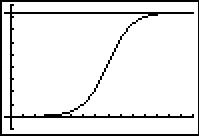
\includegraphics[width=2in]{./ExpLogsGraphics/Applications01.jpg} &

\hspace{0.75in} 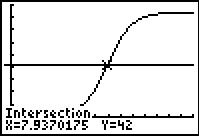
\includegraphics[width=2in]{./ExpLogsGraphics/Applications02.jpg} \\

$y = f(x) = \frac{84}{1+2799e^{-x}}$ and   & 

 \hspace{0.75in}  $y = f(x) = \frac{84}{1+2799e^{-x}}$ and \\
 
 $y = 84$ & 
 \hspace{0.75in} $y = 42$  \\

\end{tabular}

\end{center}

\end{enumerate}

\qed

\end{ex}

If we take the time to analyze the graph of $y=N(x)$ above, we can see graphically how logistic growth combines  features of uninhibited and limited growth.  The curve seems to rise steeply, then at some point, begins to level off.  The point at which this happens is called an \index{inflection point} \index{point of diminishing returns} \textbf{inflection point} or is sometimes called the `point of diminishing returns'.  At this point, even though the function is still increasing, the rate at which it does so begins to decline.  It turns out the point of diminishing returns always occurs at half the limiting population.  (In our case, when $y=42$.)  While these concepts are more precisely quantified using Calculus, below are two views of the graph of $y=N(x)$, one on the interval $[0,8]$, the other on $[8,15]$. The former looks strikingly like uninhibited growth; the latter like limited growth.

\begin{center}

\begin{tabular}{cc}

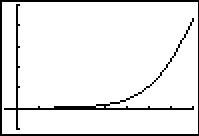
\includegraphics[width=2in]{./ExpLogsGraphics/Applications03.jpg} &

\hspace{0.75in} 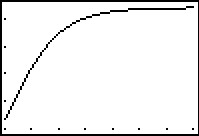
\includegraphics[width=2in]{./ExpLogsGraphics/Applications04.jpg} \\

$y = f(x) = \frac{84}{1+2799e^{-x}}$ for   & 

 \hspace{0.75in}  $y = f(x) = \frac{84}{1+2799e^{-x}}$ for \\
 
 $0 \leq x \leq 8$ & 
 \hspace{0.75in} $8 \leq x \leq 16$  \\

\end{tabular}

\end{center}


\subsection{Applications of Logarithms}

Just as many physical phenomena can be modeled by exponential functions, the same is true of logarithmic functions.   In Exercises \ref{Richterexercise},  \ref{decibelexercise} and \ref{pHexercise} of Section \ref{IntroExpLogs}, we showed that logarithms are useful in measuring the intensities of earthquakes (the Richter scale), sound (decibels) and acids and bases (pH).  We now present yet a different use of the a basic logarithm function, \href{http://en.wikipedia.org/wiki/Password_strength}{\underline{password strength}}.

\begin{ex}  The \href{http://en.wikipedia.org/wiki/Information_entropy}{\underline{information entropy}} $H$, in bits, of a randomly generated password consisting of $L$ characters is given by $H = L \log_{2}(N)$, where $N$ is the number of possible symbols for each character in the password.  In general, the higher the entropy, the stronger the password. \index{password strength} \index{information entropy}

\begin{enumerate}

\item  If a $7$ character case-sensitive\footnote{That is, upper and lower case letters are treated as different characters.} password is comprised of  letters and numbers only, find the associated information entropy.

\item  How many possible symbol options per character is required to produce a $7$ character password with an information entropy of $50$ bits?

\end{enumerate}

{\bf Solution.}

\begin{enumerate}

\item  There are $26$ letters in the alphabet, $52$ if upper and lower case letters are counted as different.  There are $10$ digits ($0$ through $9$) for a total of $N=62$ symbols.  Since the password is to be $7$ characters long, $L = 7$.  Thus, $H = 7 \log_{2}(62) = \frac{7 \ln(62)}{\ln(2)} \approx 41.68$.

\item  We have $L = 7$ and $H=50$ and we need to find $N$.  Solving the equation $50 = 7 \log_{2}(N)$ gives $N = 2^{50/7} \approx 141.323$, so we would need $142$ different symbols to choose from.\footnote{Since there are only $94$ distinct ASCII keyboard characters, to achieve this strength, the number of characters in the password should be increased.} \qed

\end{enumerate}

\end{ex}


Chemical systems known as \href{http://en.wikipedia.org/wiki/Buffer_solutions}{\underline{buffer solutions}} \index{buffer solution} have the ability to adjust to small changes in acidity to maintain a range of pH values.  Buffer solutions have a wide variety of applications from maintaining a healthy fish tank to regulating the pH levels in blood.  Our next example shows how the pH in a buffer solution is a little more complicated than the pH we first encountered in Exercise \ref{pHexercise} in Section \ref{IntroExpLogs}. 

\begin{ex}  Blood is a buffer solution. When carbon dioxide is absorbed into the bloodstream it produces carbonic acid and lowers the pH.  The body compensates by producing bicarbonate, a weak base to partially neutralize the acid.  The equation\footnote{Derived from the \href{http://en.wikipedia.org/wiki/Henderson-Hasselbalch_equation}{\underline{Henderson-Hasselbalch Equation}}. See Exercise \ref{HendersonHasselbalch} in Section \ref{LogProperties}.  Hasselbalch himself was studying carbon dioxide dissolving in blood - a process called \href{http://en.wikipedia.org/wiki/Metabolic_acidosis}{\underline{metabolic acidosis}}.}   which models blood pH in this situation is $\mbox{pH} = 6.1 + \log\left(\frac{800}{x} \right)$, where $x$ is the partial pressure of carbon dioxide in arterial blood, measured in torr. Find the partial pressure of carbon dioxide in arterial blood if the pH is $7.4$.

\smallskip

{\bf Solution.}  We set $\mbox{pH} = 7.4$ and get $ 7.4 = 6.1 + \log\left(\frac{800}{x} \right)$, or $\log\left(\frac{800}{x} \right) = 1.3$.  Solving, we find $x = \frac{800}{10^{1.3}} \approx 40.09$.  Hence, the partial pressure of carbon dioxide in the blood is about $40$ torr. \qed


\end{ex}

Another place logarithms are used is in data analysis. Suppose, for instance, we wish to model the spread of influenza A (H1N1), the so-called `Swine Flu'.  Below is data taken from the World Health Organization (\href{http://www.who.int/csr/disease/swineflu/updates/en/index.html}{\underline{WHO}}) where $t$ represents the number of days since April 28, 2009, and $N$ represents the number of confirmed cases of H1N1 virus worldwide.

\[ \begin{array}{|c||c|c|c|c|c|c|c|c|c|c|c|c|c|}  \hline

t & 1 & 2 & 3 & 4 & 5 & 6 & 7 & 8 & 9 & 10 & 11 & 12 & 13  \\ \hline

N & 148 & 257 &   367 & 658 & 898 & 1085 & 1490 & 1893 & 2371 & 2500 & 3440 & 4379 & 4694  \\ \hline \end{array} \]


\[\begin{array}{|c||c||c|c|c|c|c|c|} \hline

t & 14 & 15 & 16 & 17 & 18 & 19& 20  \\ \hline 

N & 5251 & 5728 & 6497 & 7520 & 8451 & 8480 & 8829    \\ \hline \end{array} \]

Making a scatter plot of the data treating $t$ as the independent variable and $N$ as the dependent variable gives

\centerline{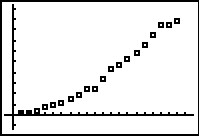
\includegraphics[width=2in]{./ExpLogsGraphics/Applications05.jpg}}

Which models are suggested by the shape of the data?  Thinking back Section \ref{Regression}, we try a Quadratic Regression, with pretty good results.

\begin{center}

\begin{tabular}{cc}

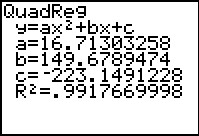
\includegraphics[width=2in]{./ExpLogsGraphics/Applications06.jpg} &

\hspace{0.75in} 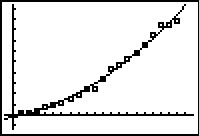
\includegraphics[width=2in]{./ExpLogsGraphics/Applications07.jpg} \\

\end{tabular}

\end{center}

However, is there any scientific reason for the data to be quadratic?  Are there other models which fit the data equally well, or better?  Scientists often use logarithms in an attempt to `linearize' data sets - in other words, transform the data sets to produce ones which result in straight lines.  To see how this could work, suppose we guessed the relationship between $N$ and $t$ was some kind of power function, not necessarily quadratic, say $N = B t^{A}$.  To try to determine the $A$ and $B$, we can take the natural log of both sides and get $\ln(N) = \ln\left(B t^{A}\right)$.  Using properties of logs to expand the right hand side of this equation, we get $\ln(N) = A \ln(t) + \ln(B)$.  If we set $X = \ln(t)$ and $Y = \ln(N)$, this equation becomes $Y = AX + \ln(B)$.  In other words, we have a line with slope $A$ and $Y$-intercept $\ln(B)$.  So, instead of plotting $N$ versus $t$, we plot $\ln(N)$ versus $\ln(t)$.

\[ \begin{array}{|c||c|c|c|c|c|c|c|c|c|c|c|c|c|}  \hline

\ln(t) & 0 & 0.693 & 1.099 & 1.386& 1.609 & 1.792 & 1.946 & 2.079 & 2.197 & 2.302 & 2.398 & 2.485 & 2.565  \\ \hline

\ln(N) & 4.997  & 5.549 &  5.905 & 6.489 & 6.800 & 6.989 & 7.306 & 7.546 & 7.771 & 7.824 & 8.143 & 8.385 & 8.454  \\ \hline \end{array} \]


\[\begin{array}{|c||c||c|c|c|c|c|c|} \hline

\ln(t) & 2.639 & 2.708 & 2.773 & 2.833 & 2.890 & 2.944 & 2.996  \\ \hline 

\ln(N) & 8.566 & 8.653 & 8.779 & 8.925 & 9.042 & 9.045 & 9.086    \\ \hline \end{array} \]

Running a linear regression on the data gives

\begin{center}

\begin{tabular}{cc}

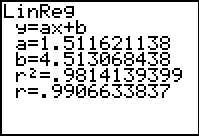
\includegraphics[width=2in]{./ExpLogsGraphics/Applications08.jpg} &

\hspace{0.75in} 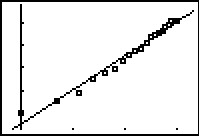
\includegraphics[width=2in]{./ExpLogsGraphics/Applications09.jpg} \\

\end{tabular}

\end{center}

The slope of the regression line is $a \approx 1.512$ which corresponds to our exponent $A$.  The $y$-intercept $b \approx 4.513$ corresponds to $\ln(B)$, so that $B \approx 91.201$.  Hence, we get the model $N = 91.201 t^{1.512}$, something from Section \ref{AlgebraicFunctions}.  Of course, the calculator has a built-in `Power Regression' feature.  If we apply this to our original data set, we get the same model we arrived at before.\footnote{Critics may question why the authors of the book have chosen to even discuss linearization of data when the calculator has a Power Regression built-in and ready to go.  Our response:  talk to your science faculty.}


\begin{center}

\begin{tabular}{cc}

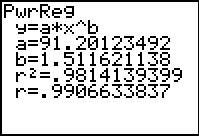
\includegraphics[width=2in]{./ExpLogsGraphics/Applications10.jpg} &

\hspace{0.75in} 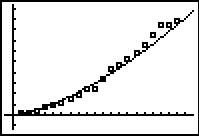
\includegraphics[width=2in]{./ExpLogsGraphics/Applications11.jpg} \\

\end{tabular}

\end{center}

This is all well and good, but the quadratic model appears to fit the data better, and we've yet to mention any scientific principle which would lead us to believe the actual spread of the flu follows any kind of power function at all.  If we are to attack this data from a scientific perspective, it does seem to make sense that, at least in the early stages of the outbreak, the more people who have the flu, the faster it will spread, which leads us to proposing an uninhibited growth model. If we assume $N = B e^{At}$ then, taking logs as before, we get $\ln(N) = At + \ln(B)$.  If we set $X = t$ and $Y = \ln(N)$, then, once again, we get $Y = AX + \ln(B)$, a line with slope $A$ and $Y$-intercept $\ln(B)$.  Plotting $\ln(N)$ versus $t$ gives the following linear regression.  

\phantomsection
\label{swineflulinearized}

\begin{center}

\begin{tabular}{cc}

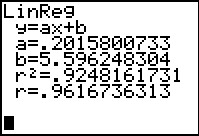
\includegraphics[width=2in]{./ExpLogsGraphics/Applications12.jpg} &

\hspace{0.75in} 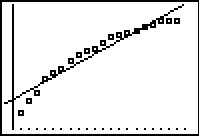
\includegraphics[width=2in]{./ExpLogsGraphics/Applications13.jpg} \\

\end{tabular}

\end{center}

We see the slope is  $a \approx 0.202$ and which corresponds to $A$ in our model, and the $y$-intercept is $b \approx 5.596$ which corresponds to $\ln(B)$.  We get $B \approx 269.414$, so that our model is $N = 269.414e^{0.202t}$. Of course, the calculator has a built-in `Exponential Regression' feature which produces what appears to be a different model $N = 269.414 (1.22333419)^{t}$.  Using properties of exponents, we write $e^{0.202t} = \left(e^{0.202}\right)^t \approx (1.223848)^{t}$, which, had we carried more decimal places, would have matched the base of the calculator model exactly.

 
\begin{center}

\begin{tabular}{cc}

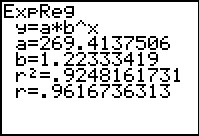
\includegraphics[width=2in]{./ExpLogsGraphics/Applications14.jpg} &

\hspace{0.75in} 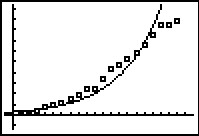
\includegraphics[width=2in]{./ExpLogsGraphics/Applications15.jpg} \\

\end{tabular}

\end{center}

The exponential model didn't fit the data as well as the quadratic or power function model, but it stands to reason that, perhaps, the spread of the flu is not unlike that of the spread of a rumor and that a logistic model can be used to model the data.  The calculator does have a `Logistic Regression' feature, and using it produces the model $N = \frac{10739.147}{1 + 42.416 e^{0.268 t}}$.

\begin{center}

\begin{tabular}{cc}

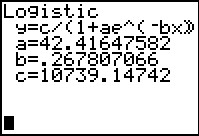
\includegraphics[width=2in]{./ExpLogsGraphics/Applications16.jpg} &

\hspace{0.75in} 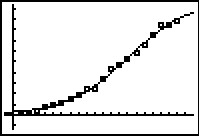
\includegraphics[width=2in]{./ExpLogsGraphics/Applications17.jpg} \\

\end{tabular}

\end{center}

This appears to be an excellent fit, but there is no friendly coefficient of determination, $R^2$, by which to judge this numerically.  There are good reasons for this, but they are far beyond the scope of the text.  Which of the models, quadratic, power, exponential, or logistic is the `best model'?  If by `best' we mean `fits closest to the data,' then the quadratic and logistic models are arguably the winners with the power function model a close second.  However, if we think about the science behind the spread of the flu, the logistic model gets an edge.  For one thing, it takes into account that only a finite number of people will ever get the flu (according to our model, $10,\!739$), whereas the quadratic model predicts no limit to the number of cases. As we have stated several times before in the text, mathematical models, regardless of their sophistication, are just that:  models, and they all have their limitations.\footnote{Speaking of limitations, as of June 3, 2009, there were 19,273 confirmed cases of influenza A (H1N1).  This is well above our prediction of 10,739.  Each time a new report is issued, the data set increases and the model must be recalculated.  We leave this recalculation to the reader.}

\newpage

\subsection{Exercises}

For each of the scenarios given in Exercises \ref{basicinterestexfirst} - \ref{basicinterestexlast}, 

\begin{itemize}

\item  Find the amount $A$ in the account as a function of the term of the investment $t$ in years. 

\item  Determine how much is in the account after $5$ years, $10$ years, $30$ years and $35$ years.  Round your answers to the nearest cent.

\item  Determine how long will it take for the initial investment to double.  Round your answer to the nearest year.

\item  Find and interpret the average rate of change of the amount in the account from the end of
the fourth year to the end of the fifth year, and from the end of the thirty-fourth year to the
end of the thirty-fifth year.  Round your answer to two decimal places.

\end{itemize} 

\begin{enumerate}

\item  $\$500$ is invested in an account which offers $0.75 \%$, compounded monthly. \label{basicinterestexfirst}

\item  $\$500$ is invested in an account which offers $0.75 \%$, compounded continuously.

\item  $\$1000$ is invested in an account which offers $1.25 \%$, compounded monthly.

\item  $\$1000$ is invested in an account which offers $1.25 \%$, compounded continuously.

\item  $\$5000$ is invested in an account which offers $2.125 \%$, compounded monthly.

\item  $\$5000$ is invested in an account which offers $2.125 \%$, compounded continuously. \label{basicinterestexlast}

\setcounter{HW}{\value{enumi}}
\end{enumerate}

\begin{enumerate}
\setcounter{enumi}{\value{HW}}

\item  Look back at your answers to Exercises \ref{basicinterestexfirst} - \ref{basicinterestexlast}. What can be said about the difference between monthly compounding and continuously compounding the interest in those situations?  With the help of your classmates, discuss scenarios where the difference between monthly  and continuously compounded interest would be more dramatic.  Try varying the interest rate, the term of the investment and the principal.  Use computations to support your answer.

\item  How much money needs to be invested now to obtain $\$2000$ in 3 years if the interest rate in a savings account is $0.25 \%$, compounded continuously?  Round your answer to the nearest cent.

\item  How much money needs to be invested now to obtain $\$5000$ in  10 years if the interest rate in a CD is $2.25 \%$, compounded monthly?  Round your answer to the nearest cent.


\item On May, 31, 2009, the Annual Percentage Rate listed at Jeff's bank for regular savings accounts was $0.25\%$ compounded monthly.  Use Equation \ref{compoundinterest} to answer the following.

\begin{enumerate}

\item If $P = 2000$ what is $A(8)$?
\item Solve the equation $A(t) = 4000$ for $t$.
\item What principal $P$ should be invested so that the account balance is \$2000 is three years?

\end{enumerate}

\item Jeff's bank also offers a 36-month Certificate of Deposit (CD) with an APR of $2.25\%$.

\begin{enumerate}

\item If $P = 2000$ what is $A(8)$?
\item Solve the equation $A(t) = 4000$ for $t$.
\item What principal $P$ should be invested so that the account balance is \$2000 in three years?
\item The Annual Percentage Yield is the \underline{simple} interest rate that returns the same amount of interest after one year as the compound interest does.  With the help of your classmates, compute the APY for this investment.

\end{enumerate}


\item  A finance company offers a promotion on $\$5000$ loans.  The borrower does not have to make any payments for the first three years, however interest will continue to be charged to the loan at $29.9 \%$ compounded continuously.  What amount will be due at the end of the three year period, assuming no payments are made?  If the promotion is extended an additional three years, and no payments are made, what amount would be due?

\item Use Equation \ref{compoundinterest} to show that the time it takes for an investment to double in value does \underline{not} depend on the principal $P$, but rather, depends only on the APR and the number of compoundings per year.  Let $n = 12$ and with the help of your classmates compute the doubling time for a variety of rates $r$.  Then look up the Rule of 72 and compare your answers to what that rule says.  If you're really interested\footnote{Awesome pun!} in Financial Mathematics, you could also compare and contrast the Rule of 72 with the Rule of 70 and the Rule of 69.

\setcounter{HW}{\value{enumi}}
\end{enumerate}

In Exercises \ref{radioactivefirst} - \ref{radioactivelast},  we list some radioactive isotopes and their associated half-lives.  Assume that each decays according to the formula $A(t) = A_{\text{\tiny $0$}}e^{kt}$ where $A_{\text{\tiny $0$}}$ is the initial amount of the material and $k$ is the decay constant. For each isotope:

\begin{itemize}

\item  Find the decay constant $k$.  Round your answer to four decimal places.

\item  Find a function which gives the amount of isotope $A$ which remains after time $t$.  (Keep the units of $A$ and $t$ the same as the given data.)

\item  Determine how long it takes for $90 \%$ of the material to decay.  Round your answer to two decimal places.  (HINT:  If $90 \%$ of the material decays, how much is left?)

\end{itemize}

\begin{enumerate}
\setcounter{enumi}{\value{HW}}

\item  Cobalt 60, used in food irradiation, initial amount 50 grams, half-life of $5.27$ years.  \label{radioactivefirst}

\item  Phosphorus 32, used in agriculture, initial amount 2 milligrams, half-life $14$ days.

\item  Chromium 51, used to track red blood cells, initial amount 75 milligrams, half-life  $27.7$ days.

\item  Americium 241, used in smoke detectors, initial amount 0.29 micrograms, half-life $432.7$ years.

\item  Uranium 235, used for nuclear power, initial amount $1$ kg grams, half-life  $704$ million years. \label{radioactivelast}

\setcounter{HW}{\value{enumi}}
\end{enumerate}

\begin{enumerate}
\setcounter{enumi}{\value{HW}}

\item With the help of your classmates, show that the time it takes for $90 \%$ of each isotope listed in Exercises \ref{radioactivefirst} - \ref{radioactivelast} to decay does not depend on the initial amount of the substance, but rather, on only the decay constant $k$. Find a formula, in terms of $k$ only, to determine how long it takes for $90 \%$ of a radioactive isotope to decay. 


\item In Example \ref{cardepreciationex} in Section \ref{IntroExpLogs}, the exponential function $V(x) = 25 \left(\frac{4}{5}\right)^{x}$ was used to model the value of a car over time.  Use the properties of logs and/or exponents to rewrite the model in the form $V(t) = 25e^{kt}$.

\item  The Gross Domestic Product (GDP) of the US (in billions of dollars) $t$ years after the year 2000 can be modeled by: \[ G(t) = 9743.77 e^{0.0514t}\]

\begin{enumerate}

\item  Find and interpret $G(0)$.

\item  According to the model, what should have been the GDP in 2007?  In 2010?  (According to the   \href{http://1.usa.gov/iimT40}{\underline{US Department of Commerce}}, the 2007 GDP was $\$14,369.1$ billion and the 2010 GDP was $\$14,657.8$ billion.)

\end{enumerate}

\item  The diameter $D$ of a tumor, in millimeters, $t$ days after it is detected is given by:  \[D(t) = 15e^{0.0277t} \]

\begin{enumerate}

\item  What was the diameter of the tumor when it was originally detected?

\item  How long until the diameter of the tumor doubles?

\end{enumerate}

\item  Under optimal conditions, the growth of a certain strain of \textit{E. Coli} is modeled by the Law of Uninhibited Growth $N(t) = N_{\text{\tiny $0$}} e^{kt}$ where $N_{\text{\tiny $0$}}$ is the initial number of bacteria and $t$ is the elapsed time, measured in minutes. From numerous experiments, it has been determined that the doubling time of this organism is 20 minutes. Suppose 1000 bacteria are present initially.

\begin{enumerate}

\item  Find the growth constant $k$. Round your answer to four decimal places.

\item  Find a function which gives the number of bacteria $N(t)$ after $t$ minutes.

\item  How long until there are 9000 bacteria?  Round your answer to the nearest minute.

\end{enumerate}

\item  Yeast is often used in biological experiments.  A research technician estimates that a sample of yeast suspension contains 2.5 million organisms per cubic centimeter (cc).  Two hours later, she estimates the population density to be 6 million organisms per cc.  Let $t$ be the time elapsed since the first observation, measured in hours.  Assume that the yeast growth follows the Law of Uninhibited Growth $N(t) = N_{\text{\tiny $0$}} e^{kt}$.

\begin{enumerate}

\item  Find the growth constant $k$. Round your answer to four decimal places.

\item  Find a function which gives the number of yeast (in millions) per cc $N(t)$ after $t$ hours.

\item  What is the doubling time for this strain of yeast?

\end{enumerate}


\item  The Law of Uninhibited Growth also applies to situations where an animal is re-introduced into a suitable environment.  Such a case is the reintroduction of wolves to Yellowstone National Park.   According to the \href{http://www.nps.gov/yell/naturescience/wolves.htm}{\underline{National Park Service}}, the wolf population in Yellowstone National Park was 52 in 1996 and 118 in 1999.  Using these data, find a function of the form $N(t) = N_{\text{\tiny $0$}} e^{kt}$  which models the number of wolves $t$ years after 1996.  (Use $t = 0$ to represent the year 1996.  Also, round your value of $k$ to four decimal places.)  According to the model, how many wolves were in Yellowstone in 2002?  (The recorded number is 272.)

\item  \label{PainesvillePopulationTwoPoint} During the early years of a community, it is not uncommon for the population to grow according to the Law of Uninhibited Growth.  According to the Painesville Wikipedia entry, in 1860, the Village of Painesville had a population of 2649.  In 1920, the population was 7272.  Use these two data points to fit a model of the form $N(t) = N_{\text{\tiny $0$}} e^{kt}$ were $N(t)$ is the number of Painesville Residents $t$ years after 1860.  (Use $t = 0$ to represent the year 1860.  Also, round the value of $k$ to four decimal places.)  According to this model, what was the population of Painesville in 2010?  (The 2010 census gave the population as 19,563) What could be some causes for such a vast discrepancy?  For more on this, see Exercise \ref{PainesvillePopulationManyPoints}.

\item  The population of Sasquatch in Bigfoot county is modeled by \[P(t) = \dfrac{120}{1 + 3.167e^{-0.05t}}\] where $P(t)$ is the population of Sasquatch $t$ years after $2010$.

\begin{enumerate}

\item  Find and interpret $P(0)$.

\item  Find the population of Sasquatch in Bigfoot county in 2013.  Round your answer to the nearest Sasquatch.

\item  When will the population of Sasquatch in Bigfoot county reach 60?  Round your answer to the nearest year.

\item  Find and interpret the end behavior of the graph of $y = P(t)$.  Check your answer using a graphing utility. 

\end{enumerate}

\setcounter{HW}{\value{enumi}}
\end{enumerate}


\begin{enumerate}
\setcounter{enumi}{\value{HW}}


\item The half-life of the radioactive isotope Carbon-14 is about 5730 years.  

\begin{enumerate}

\item Use Equation \ref{radioactivedecay} to express the amount of Carbon-14 left from an initial $N$ milligrams as a function of time $t$ in years.

\item What percentage of the original amount of Carbon-14 is left after 20,000 years?

\item If an old wooden tool is found in a cave and the amount of Carbon-14 present in it is estimated to be only 42\% of the original amount, approximately how old is the tool?

\item Radiocarbon dating is not as easy as these exercises might lead you to believe.  With the help of your classmates, research radiocarbon dating and discuss why our model is somewhat over-simplified.  

\end{enumerate}

\item Carbon-14 cannot be used to date inorganic material such as rocks, but there are many other methods of radiometric dating which estimate the age of rocks.  One of them, Rubidium-Strontium dating, uses Rubidium-87 which decays to Strontium-87 with a half-life of 50 billion years.  Use Equation \ref{radioactivedecay} to express the amount of Rubidium-87 left from an initial 2.3 micrograms as a function of time $t$ in \emph{billions} of years.  Research this and other radiometric techniques and discuss the margins of error for various methods with your classmates.

\item Use Equation \ref{radioactivedecay} to show that $k = -\dfrac{\ln(2)}{h}$ where $h$ is the half-life of the radioactive isotope.


\item A pork roast\footnote{This roast was enjoyed by Jeff and his family on June 10, 2009.  This is real data, folks!} was taken out of a hardwood smoker when its internal temperature had reached $180^{\circ}$F and it was allowed to rest in a $75^{\circ}$F house for 20 minutes after which its internal temperature had dropped to $170^{\circ}$F. Assuming that the temperature of the roast follows Newton's Law of Cooling (Equation \ref{newtonslawofcooling}),

\begin{enumerate}

\item Express the temperature $T$ (in $^{\circ}$F) as a function of time $t$ (in minutes).

\item Find the time at which the roast would have dropped to $140^{\circ}$F had it not been carved and eaten. 

\end{enumerate}

\item  \label{pursuitlog} In reference to Exercise \ref{pursuitfurther} in Section \ref{AlgebraicFunctions}, if Fritzy the Fox's speed is the same as Chewbacca the Bunny's speed, Fritzy's pursuit curve is given by

\[y(x) = \frac{1}{4} x^2-\frac{1}{4} \ln(x)-\frac{1}{4}\]

Use your calculator to graph this path for $x > 0$.  Describe the behavior of $y$ as $x \rightarrow 0^{+}$ and interpret this physically.

\item \label{explogsappcircuitone} The current $i$ measured in amps in a certain electronic circuit with a constant impressed voltage of 120 volts is given by $i(t) = 2 - 2e^{-10t}$ where $t \geq 0$ is the number of seconds after the circuit is switched on.  Determine the value of $i$ as $t \rightarrow \infty$.  (This is called the \textbf{steady state} current.)


\item If the voltage in the circuit in Exercise \ref{explogsappcircuitone} above is switched off after 30 seconds, the current is given by the piecewise-defined function 

\[i(t) = \left\{ \begin{array}{rcl} 2 - 2e^{-10t} & \mbox{if} & 0 \leq t < 30 \\ [6pt]
\left(2 - 2e^{-300}\right) e^{-10t+300} & \mbox{if} & t \geq 30 \end{array} \right.\]  

With the help of your calculator, graph $y = i(t)$ and discuss with your classmates the physical significance of the two parts of the graph $0 \leq t < 30$ and $t \geq 30$.

\item \label{catenary} In Exercise \ref{parabolicbridgecable} in Section \ref{QuadraticFunctions}, we stated that the cable of a suspension bridge formed a parabola but that a free hanging cable did not.  A free hanging cable forms a \underline{catenary} and its basic shape is given by $y = \frac{1}{2}\left(e^{x} + e^{-x}\right)$.  Use your calculator to graph this function.  What are its domain and range?  What is its end behavior?  Is it invertible?  How do you think it is related to the function given in Exercise \ref{hyperbolicsine} in Section \ref{ExpEquations} and the one given in the answer to Exercise \ref{inversehyptangent} in Section \ref{LogEquations}?  When flipped upside down, the catenary makes an arch.  The Gateway Arch in St. Louis, Missouri has the shape \[y = 757.7 - \frac{127.7}{2}\left(e^{\frac{x}{127.7}} + e^{-\frac{x}{127.7}}\right)\] where $x$ and $y$ are measured in feet and $-315 \leq x \leq 315$.  Find the highest point on the arch.

\item In Exercise \ref{APLcats} in Section \ref{Regression}, we examined the data set given below which showed how two cats and their surviving offspring can produce over 80 million cats in just ten years.  It is virtually impossible to see this data plotted on your calculator, so plot $x$ versus $\ln(x)$ as was done on page \pageref{swineflulinearized}.  Find a linear model for this new data and comment on its goodness of fit.  Find an exponential model for the original data and comment on its goodness of fit.

\medskip

\small

\noindent \begin{tabular}{|l|r|r|r|r|r|r|r|r|r|r|} \hline
Year $x$ & 1 & 2 & 3 & 4 & 5 & 6 & 7 & 8 & 9 & 10 \\ 
\hline 
Number of  & & & & & & & & & & \\
Cats $N(x)$ & 12 & 66 & 382 & 2201 & 12680 & 73041 & 420715 & 2423316 & 13968290 & 80399780 \\ \hline
\end{tabular}

\normalsize


\item  \label{PainesvillePopulationManyPoints} This exercise is a follow-up to Exercise \ref{PainesvillePopulationTwoPoint} which more thoroughly explores the population growth of Painesville, Ohio.  According to \href{http://en.wikipedia.org/wiki/Painesville}{\underline{Wikipedia}}, the population of Painesville, Ohio is given by


\noindent \begin{tabular}{|l|r|r|r|r|r|r|r|r|r|r|} \hline
Year $t$ & 1860 & 1870 & 1880 & 1890 & 1900 & 1910 & 1920 & 1930 & 1940 & 1950 \\ \hline 
Population& 2649 & 3728 & 3841 & 4755 & 5024 & 5501 & 7272 & 10944 & 12235 & 14432 \\ \hline
\end{tabular}

\noindent \begin{tabular}{|l|r|r|r|r|r|} \hline
Year $t$ & 1960 & 1970 & 1980 & 1990 & 2000 \\ \hline 
Population& 16116 & 16536 & 16351 & 15699 & 17503 \\ \hline
\end{tabular}

\begin{enumerate}

\item  Use a graphing utility to perform an exponential regression on the data from 1860 through 1920 only, letting $t = 0$ represent the year 1860 as before.  How does this calculator model compare with the model you found in Exercise \ref{PainesvillePopulationTwoPoint}?   Use the calculator's exponential model to predict the population in 2010.   (The 2010 census gave the population as 19,563)

\item  The logistic model fit to \emph{all} of the given data points for the population of Painesville $t$ years after 1860 (again, using $t = 0$ as 1860) is \[ P(t) = \dfrac{18691}{1+9.8505e^{-0.03617t}} \] According to this model, what should the population of Painesville have been in 2010?  (The 2010 census gave the population as 19,563.) What is the population limit of Painesville?

\end{enumerate}



\item  According to \href{http://www.ohiobiz.com/census/Lake.pdf}{\underline{OhioBiz}}, the census data for Lake County, Ohio is as follows:

\small
\noindent \begin{tabular}{|l|r|r|r|r|r|r|r|r|r|r|} \hline
Year $t$ & 1860 & 1870 & 1880 & 1890 & 1900 & 1910 & 1920 & 1930 & 1940 & 1950 \\ \hline 
Population& 15576 & 15935 & 16326 & 18235 & 21680 & 22927 & 28667 & 41674 & 50020 & 75979 \\ \hline
\end{tabular}

\noindent \begin{tabular}{|l|r|r|r|r|r|} \hline
Year $t$ & 1960 & 1970 & 1980 & 1990 & 2000 \\ \hline 
Population& 148700 & 197200 & 212801 & 215499 & 227511 \\ \hline
\end{tabular}

\normalsize

\begin{enumerate}

\item  Use your calculator to fit a logistic model to these data, using $x = 0$ to represent the year 1860. 

\item  Graph these data and your logistic function on your calculator to judge the reasonableness of the fit.

\item  Use this model to estimate the population of Lake County in 2010.  (The 2010 census gave the population to be 230,041.)

\item  According to your model, what is the population limit of Lake County, Ohio?

\end{enumerate}



\item According to \href{http://www.facebook.com/press/info.php?timeline}{\underline{facebook}}, the number of active users of facebook has grown significantly since its initial launch from a Harvard dorm room in February 2004. The chart below has the approximate number $U(x)$ of active users, in \underline{millions}, $x$ months after February 2004.  For example, the first entry $(10, 1)$ means that there were $1$ million active users in December 2004 and the last entry $(77, 500)$ means that there were $500$ million active users in July 2010.

\medskip
\small
\noindent \begin{tabular}{|l|r|r|r|r|r|r|r|r|r|r|r|r|r|r|} \hline
Month $x$ & 10 & 22 & 34 & 38 & 44 & 54 & 59 & 60 & 62 & 65 & 67 & 70 & 72 & 77 \\ \hline 
Active Users in & & & & & & & & & & & & & & \\
Millions $U(x)$ & 1 & 5.5 & 12 & 20 & 50 & 100 & 150 & 175 & 200 & 250 & 300 & 350 & 400 & 500\\ \hline
\end{tabular}
\normalsize
\medskip

With the help of your classmates, find a model for this data.

\item Each Monday during the registration period before the Fall Semester at LCCC, the Enrollment Planning Council gets a report prepared by the data analysts in Institutional Effectiveness and Planning.\footnote{The authors thank Dr. Wendy Marley and her staff for this data and Dr. Marcia Ballinger for the permission to use it in this problem.}  While the ongoing enrollment data is analyzed in many different ways, we shall focus only on the overall headcount.  Below is a chart of the enrollment data for Fall Semester 2008.  It starts 21 weeks before ``Opening Day'' and ends on ``Day 15'' of the semester, but we have relabeled the top row to be $x = 1$ through $x = 24$ so that the math is easier.  (Thus, $x = 22$ is Opening Day.)


\noindent \begin{tabular}{|l|r|r|r|r|r|r|r|r|} \hline
Week $x$ & 1 & 2 & 3 & 4 & 5 & 6 & 7 & 8 \\ \hline 
Total  & & & & & & & & \\
Headcount & 1194 & 1564 & 2001 & 2475 & 2802 & 3141 & 3527 & 3790 \\ \hline
\end{tabular}

\medskip

\noindent \begin{tabular}{|l|r|r|r|r|r|r|r|r|} \hline
Week $x$ & 9 & 10 & 11 & 12 & 13 & 14 & 15 & 16 \\ \hline 
Total  & & & & & & & & \\
Headcount & 4065 & 4371 & 4611 & 4945 & 5300 & 5657 & 6056 & 6478 \\ \hline
\end{tabular}

\medskip

\noindent \begin{tabular}{|l|r|r|r|r|r|r|r|r|} \hline
Week $x$ & 17 & 18 & 19 & 20 & 21 & 22 & 23 & 24\\ \hline 
Total  & & & & & & & & \\
Headcount & 7161 & 7772 & 8505 & 9256 & 10201 & 10743 & 11102 & 11181 \\ \hline
\end{tabular}

\medskip

With the help of your classmates, find a model for this data.  Unlike most of the phenomena we have studied in this section, there is no single differential equation which governs the enrollment growth.  Thus there is no scientific reason to rely on a logistic function even though the data plot may lead us to that model.  What are some factors which influence enrollment at a community college and how can you take those into account mathematically?  

\item When we wrote this exercise, the Enrollment Planning Report for Fall Semester 2009 had only 10 data points for the first 10 weeks of the registration period.  Those numbers are given below.  

\noindent \begin{tabular}{|l|r|r|r|r|r|r|r|r|r|r|} \hline
Week $x$ & 1 & 2 & 3 & 4 & 5 & 6 & 7 & 8 & 9 & 10 \\ \hline 
Total  & & & & & & & & & & \\
Headcount & 1380 & 2000 & 2639 & 3153 & 3499 & 3831 & 4283 & 4742 & 5123 & 5398 \\ \hline
\end{tabular}

With the help of your classmates, find a model for this data and make a prediction for the Opening Day enrollment as well as the Day 15 enrollment.  (WARNING: The registration period for 2009 was one week shorter than it was in 2008 so Opening Day would be $x = 21$ and Day 15 is $x = 23$.)


\end{enumerate}

\newpage

\subsection{Answers}

\begin{enumerate}

\item \begin{itemize}  \item $A(t) = 500\left(1 + \frac{0.0075}{12}\right)^{12t}$ 

\item $A(5) \approx \$ 519.10$, $A(10) \approx \$ 538.93$, $A(30) \approx \$ 626.12$, $A(35) \approx \$ 650.03$ 

\item It will take approximately $92$ years for the investment to double.

\item  The average rate of change from the end of the fourth year to the end of the fifth year is approximately $3.88$.  This means that the investment is growing at an average rate of $\$3.88$ per year at this point.  The average rate of change from the end of the thirty-fourth year to the end of the thirty-fifth year is approximately $4.85$.  This means that the investment is growing at an average rate of $\$4.85$ per year at this point. 

\end{itemize}

\item \begin{itemize}  \item $A(t) = 500e^{0.0075t}$ 

\item $A(5) \approx \$ 519.11$, $A(10) \approx \$ 538.94$, $A(30) \approx \$ 626.16$, $A(35) \approx \$ 650.09$ 

\item It will take approximately $92$ years for the investment to double.

\item  The average rate of change from the end of the fourth year to the end of the fifth year is approximately $3.88$.  This means that the investment is growing at an average rate of $\$3.88$ per year at this point.  The average rate of change from the end of the thirty-fourth year to the end of the thirty-fifth year is approximately $4.86$.  This means that the investment is growing at an average rate of $\$4.86$ per year at this point. 

\end{itemize}

\item \begin{itemize}  \item $A(t) = 1000\left(1 + \frac{0.0125}{12}\right)^{12t}$ 

\item $A(5) \approx \$ 1064.46$, $A(10) \approx \$ 1133.07$, $A(30) \approx \$ 1454.71$, $A(35) \approx \$ 1548.48$ 

\item  It will take approximately $55$ years for the investment to double.

\item  The average rate of change from the end of the fourth year to the end of the fifth year is approximately $13.22$.  This means that the investment is growing at an average rate of $\$13.22$ per year at this point.  The average rate of change from the end of the thirty-fourth year to the end of the thirty-fifth year is approximately $19.23$.  This means that the investment is growing at an average rate of $\$19.23$ per year at this point. 

\end{itemize}

\item \begin{itemize}  \item $A(t) = 1000e^{0.0125t}$ 

\item $A(5) \approx \$ 1064.49$, $A(10) \approx \$ 1133.15$, $A(30) \approx \$ 1454.99$, $A(35) \approx \$ 1548.83$ 

\item It will take approximately $55$ years for the investment to double.

\item  The average rate of change from the end of the fourth year to the end of the fifth year is approximately $13.22$.  This means that the investment is growing at an average rate of $\$13.22$ per year at this point.  The average rate of change from the end of the thirty-fourth year to the end of the thirty-fifth year is approximately $19.24$.  This means that the investment is growing at an average rate of $\$19.24$ per year at this point. 

\end{itemize}



\item \begin{itemize}  \item $A(t) = 5000\left(1 + \frac{0.02125}{12}\right)^{12t}$ 

\item $A(5) \approx \$ 5559.98$, $A(10) \approx \$ 6182.67$, $A(30) \approx \$ 9453.40$, $A(35) \approx \$ 10512.13$ 

\item  It will take approximately $33$ years for the investment to double.

\item  The average rate of change from the end of the fourth year to the end of the fifth year is approximately $116.80$.  This means that the investment is growing at an average rate of $\$116.80$ per year at this point.  The average rate of change from the end of the thirty-fourth year to the end of the thirty-fifth year is approximately $220.83$.  This means that the investment is growing at an average rate of $\$220.83$ per year at this point. 

\end{itemize}



\item \begin{itemize}  \item $A(t) = 5000e^{0.02125t}$ 

\item $A(5) \approx \$ 5560.50$, $A(10) \approx \$ 6183.83$, $A(30) \approx \$ 9458.73$, $A(35) \approx \$ 10519.05$ 

\item  It will take approximately $33$ years for the investment to double.

\item  The average rate of change from the end of the fourth year to the end of the fifth year is approximately $116.91$.  This means that the investment is growing at an average rate of $\$116.91$ per year at this point.  The average rate of change from the end of the thirty-fourth year to the end of the thirty-fifth year is approximately $221.17$.  This means that the investment is growing at an average rate of $\$221.17$ per year at this point. 

\end{itemize}

\setcounter{HW}{\value{enumi}}
\end{enumerate}

\begin{enumerate}
\setcounter{enumi}{\value{HW}}

\addtocounter{enumi}{1}

\item  $P = \frac{2000}{e^{0.0025 \cdot 3}} \approx \$ 1985.06$

\item  $P = \frac{5000}{\left(1 + \frac{0.0225}{12}\right)^{12 \cdot 10}} \approx \$ 3993.42$

\item \begin{enumerate}

\item $A(8) = 2000\left(1 + \frac{0.0025}{12}\right)^{12 \cdot 8} \approx \$2040.40$
\item $t = \dfrac{\ln(2)}{12 \ln\left(1 + \frac{0.0025}{12}\right)} \approx 277.29$ years
\item $P = \dfrac{2000}{\left(1 + \frac{0.0025}{12}\right)^{36}} \approx \$1985.06$

\end{enumerate}

\item \begin{enumerate}

\item $A(8) = 2000\left(1 + \frac{0.0225}{12}\right)^{12 \cdot 8} \approx \$2394.03$
\item $t = \dfrac{\ln(2)}{12 \ln\left(1 + \frac{0.0225}{12}\right)} \approx 30.83$ years
\item $P = \dfrac{2000}{\left(1 + \frac{0.0225}{12}\right)^{36}} \approx \$1869.57$
\item $\left(1 + \frac{0.0225}{12}\right)^{12} \approx 1.0227$ so the APY is 2.27\%

\end{enumerate}

\item  $A(3) = 5000e^{0.299 \cdot 3} \approx \$12,226.18$,  $A(6) = 5000e^{0.299 \cdot 6} \approx \$30,067.29$

\setcounter{HW}{\value{enumi}}
\end{enumerate}


\begin{multicols}{2}
\begin{enumerate}
\setcounter{enumi}{\value{HW}}
\addtocounter{enumi}{1}

\item  \begin{itemize}  \item $k = \frac{\ln(1/2)}{5.27} \approx -0.1315$

\item $A(t) = 50e^{-0.1315t}$

\item  $t = \frac{\ln(0.1)}{-0.1315} \approx 17.51$ years.

\end{itemize}



\item  \begin{itemize}  \item $k = \frac{\ln(1/2)}{14} \approx -0.0495$

\item $A(t) = 2e^{-0.0495t}$

\item  $t = \frac{\ln(0.1)}{-0.0495} \approx 46.52$ days.

\end{itemize}

\setcounter{HW}{\value{enumi}}
\end{enumerate}
\end{multicols}

\begin{multicols}{2}
\begin{enumerate}
\setcounter{enumi}{\value{HW}}


\item  \begin{itemize}  \item $k = \frac{\ln(1/2)}{27.7} \approx -0.0250$

\item $A(t) = 75e^{-0.0250t}$

\item  $t = \frac{\ln(0.1)}{-0.025} \approx 92.10$ days.

\end{itemize}

\item  \begin{itemize}  \item $k = \frac{\ln(1/2)}{432.7} \approx -0.0016$

\item $A(t) = 0.29e^{-0.0016t}$

\item  $t = \frac{\ln(0.1)}{-0.0016} \approx 1439.11$ years.

\end{itemize}


\setcounter{HW}{\value{enumi}}
\end{enumerate}
\end{multicols}

\begin{enumerate}
\setcounter{enumi}{\value{HW}}

\item  \begin{itemize}  \item $k = \frac{\ln(1/2)}{704} \approx -0.0010$

\item $A(t) = e^{-0.0010t}$

\item $t = \frac{\ln(0.1)}{-0.0010} \approx 2302.58$ million years, or $2.30$ billion years.

\end{itemize}


\setcounter{HW}{\value{enumi}}
\end{enumerate}

\begin{multicols}{2}
\begin{enumerate}
\setcounter{enumi}{\value{HW}}


\item  $t = \frac{\ln(0.1)}{k} = -\frac{\ln(10)}{k}$

\item $V(t) = 25e^{\ln\left(\frac{4}{5}\right)t} \approx 25e^{-0.22314355t}$

\setcounter{HW}{\value{enumi}}
\end{enumerate}
\end{multicols}


\begin{enumerate}
\setcounter{enumi}{\value{HW}}


\item \begin{enumerate}  \item  $G(0) = 9743.77$  This means that the GDP of the US in 2000 was $\$9743.77$ billion dollars.

\item  $G(7) = 13963.24$ and $G(10) = 16291.25$, so the model predicted a GDP of $\$ 13,963.24$ billion in 2007 and $\$ 16,291.25$ billion in 2010. 

\end{enumerate}

\item \begin{enumerate} \item $D(0) = 15$, so the tumor was 15 millimeters in diameter when it was first detected.

\item  $t = \frac{\ln(2)}{0.0277} \approx 25$ days.

\end{enumerate}

\setcounter{HW}{\value{enumi}}
\end{enumerate}

\begin{multicols}{2}
\begin{enumerate}
\setcounter{enumi}{\value{HW}}

\item  \begin{enumerate} \item  $k = \frac{\ln(2)}{20} \approx 0.0346$

\item  $N(t) = 1000e^{0.0346 t}$

\item  $t = \frac{\ln(9)}{0.0346} \approx 63$ minutes

\end{enumerate}

\item  \begin{enumerate} \item  $k = \frac{1}{2}\frac{\ln(6)}{2.5} \approx 0.4377$

\item  $N(t) = 2.5e^{0.4377 t}$

\item  $t = \frac{\ln(2)}{0.4377} \approx 1.58$ hours

\end{enumerate}

\setcounter{HW}{\value{enumi}}
\end{enumerate}
\end{multicols}

\begin{enumerate}
\setcounter{enumi}{\value{HW}}


\item  $N_{\text{\tiny $0$}} = 52$,  $k = \frac{1}{3} \ln\left( \frac{118}{52}\right) \approx 0.2731$, $N(t) = 52e^{0.2731t}$.  $N(6) \approx 268$. 

\item  $N_{\text{\tiny $0$}} = 2649$,  $k = \frac{1}{60} \ln\left( \frac{7272}{2649}\right) \approx 0.0168$, $N(t) = 2649e^{0.0168t}$.  $N(150) \approx 32923$, so the population of Painesville in 2010 based on this model would have been 32,923.



\item  \begin{enumerate}  \item  $P(0) = \frac{120}{4.167} \approx 29$.  There are 29 Sasquatch in Bigfoot County in 2010.

\item  $P(3) = \frac{120}{1+3.167e^{-0.05(3)}} \approx 32$ Sasquatch.

\item  $t = 20 \ln(3.167) \approx 23$ years.

\item  As $t \rightarrow \infty$, $P(t) \rightarrow 120$.  As time goes by, the Sasquatch Population in Bigfoot County will approach 120.  Graphically,  $y = P(x)$ has a horizontal asymptote $y=120$.

\end{enumerate}


\item \begin{enumerate}

\item $A(t) = Ne^{-\left(\frac{\ln(2)}{5730}\right)t} \approx Ne^{-0.00012097t}$
\item $A(20000) \approx 0.088978 \cdot N$ so about 8.9\% remains
\item $t \approx \dfrac{\ln(.42)}{-0.00012097} \approx 7171$ years old

\end{enumerate}

\item $A(t) = 2.3e^{-0.0138629t}$

\pagebreak

\addtocounter{enumi}{1}

\item \begin{enumerate}

\item $T(t) = 75 + 105e^{-0.005005t}$

\item The roast would have cooled to $140^{\circ}$F in about 95 minutes.

\end{enumerate}

\item From the graph, it appears that as $x \rightarrow 0^{+}$, $y \rightarrow \infty$.  This is due to the presence of the $\ln(x)$ term in the function.  This means that Fritzy will never catch Chewbacca, which makes sense since Chewbacca has a head start and Fritzy only runs as fast as he does.

\begin{center}

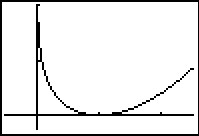
\includegraphics[width=2in]{./ExpLogsGraphics/PURSUIT03.jpg} 

\smallskip

$y(x) = \frac{1}{4} x^2-\frac{1}{4} \ln(x)-\frac{1}{4}$

\end{center}

\item The steady state current is 2 amps.

\addtocounter{enumi}{2}

\item The linear regression on the data below is $y = 1.74899x + 0.70739$ with $r^{2} \approx 0.999995$.  This is an excellent fit.

\scriptsize

\noindent \begin{tabular}{|l|r|r|r|r|r|r|r|r|r|r|} \hline
$x$ & 1 & 2 & 3 & 4 & 5 & 6 & 7 & 8 & 9 & 10 \\ 
\hline 
$\ln(N(x))$ & 2.4849 & 4.1897 & 5.9454 & 7.6967 & 9.4478 & 11.1988 & 12.9497 & 14.7006 & 16.4523 & 18.2025 \\ \hline
\end{tabular}

\normalsize

$N(x) = 2.02869(5.74879)^{x} = 2.02869e^{1.74899x}$ with $r^{2} \approx 0.999995$.  This is also an excellent fit and corresponds to our linearized model because $\ln(2.02869) \approx 0.70739$.

\item  \begin{enumerate}  \item  The calculator gives:  $y = 2895.06 (1.0147)^{x}$.  Graphing this along with our answer from Exercise \ref{PainesvillePopulationTwoPoint} over the interval $[0,60]$ shows that they are pretty close. From this model, $y(150) \approx 25840$ which once again overshoots the actual data value.

\item $P(150) \approx 18717$, so this model predicts 17,914 people in Painesville in 2010, a more conservative number than was recorded in the 2010 census.  As $t \rightarrow \infty$, $P(t) \rightarrow 18691$.  So the limiting population of Painesville based on this model is 18,691 people.

\enlargethispage{\baselineskip}

\end{enumerate}

\item \begin{enumerate}  \item  $y = \dfrac{242526}{1+874.62e^{-0.07113x}}$, where $x$ is the number of years since 1860.

\item  The plot of the data and the curve is below.

\centerline{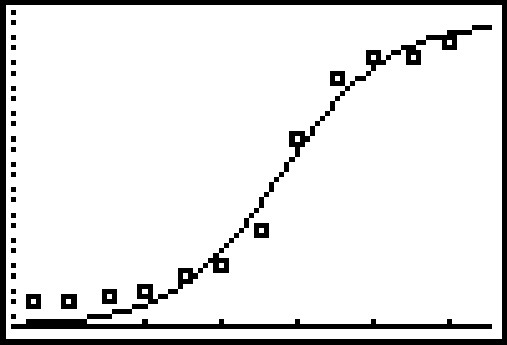
\includegraphics[width=1.75in]{./ExpLogsGraphics/LAKECOUNTYLOGISTIC.jpg} }

\item  $y(140) \approx 232889$, so this model predicts 232,889 people in Lake County in 2010.

\item  As $x \rightarrow \infty$, $y \rightarrow 242526$, so the limiting population of Lake County based on this model is 242,526 people.

\end{enumerate}

\end{enumerate}

\closegraphsfile


\end{document}